\documentclass[11pt,a4paper,twoside,openright]{book}  
%alt: [11/12pt,a4paper/letterpaper,oneside/twoside,openany/openright]{book/memoir}

%% ========================================================
%% For the cover page
%% ========================================================
% la ligne ci-dessous est à insérer obligatoirement dans le préambule du document avant \begin{document}
\usepackage[a4paper]{./cover/meta-donnees} % for the title page

%% ========================================================
%% General packages
%% ========================================================

\usepackage{times,amsmath,amssymb,amsfonts,color,graphicx,latexsym,amsthm}
% \usepackage{xcolor}
\usepackage[table,dvipsnames]{xcolor}
\usepackage{booktabs} % for better tables

\usepackage{tikz,array}
\usetikzlibrary{arrows,automata,calc,decorations.pathmorphing, backgrounds,fit, shapes}

\usepackage{algorithm, algpseudocode}
\usepackage{setspace} % used with \begin{spacing}{..}..\end{spacing}  --> needed in book
% 
\usepackage[normalem]{ulem}

\usepackage{datetime}

\graphicspath{ {figures/} }
% \usepackage{caption}
\usepackage[font={small}]{caption}
\usepackage{subcaption}
% \usepackage[labelformat=simple]{subcaption}
% \renewcommand\thesubfigure{(\alph{subfigure})}  % subfigure with parenthesis, e.g., Figure 1.2(a)
% \renewcommand\thesubfigure{-\alph{subfigure}}   % subfigure with dash, e.g., Figure 1.2-a
\usepackage{multirow}
% \captionsetup{justification=centering}
% \usepackage[caption=true]{subfig}

\usepackage{enumitem} % to change list styling globally

%% ========================================================
% % for the geometry of the pages
%% ========================================================
% \setlength{\parindent}{3.0em}
% \setlength{\parskip}{0.5em}
% \linespread{1.1}  % space between lines
% \usepackage{fullpage}  % decrease margins
% \usepackage{a4wide}
% \usepackage{showframe}   % shows the frames of the pages

%% ========================================================
% Set depth of TOC
%% ========================================================
% \setcounter{tocdepth}{2}
% \settocdepth{subsection}
% \setsecnumdepth{subsection}

%% ========================================================
%% for the mini-toc - have a toc in the beginning of each chapter
%% ========================================================
% \usepackage{minitoc}
% \setcounter{minitocdepth}{1} 
%\nomtcrule       % removes rules = horizontal lines
%\nomtcpagenumbers  % remove page numbers from minitocs
% \dominitoc %% \dominitoc[n] removes contents, \dominitoc[c] centers contents


%% ========================================================
% % %% Make an index list
%% ========================================================
% % \usepackage{imakeidx}
% % \makeindex[title=Index, options= -s ./stylefiles/myIndexStyle.ist, intoc, columns=1]


%% ========================================================
%%%% Style of Chapters 
%% ========================================================

% \usepackage[Lenny]{fncychap}
% \usepackage[Sonny]{fncychap}
% \usepackage[Rejne]{fncychap}
% \usepackage[Bjarne]{fncychap}
% \usepackage[Bjornstrup]{fncychap}
% \usepackage[Conny]{fncychap} %%  incompatible with toc


%% My STYLE
%% Set introduction chapter to 0
% \setcounter{chapter}{-1}

%% My STYLE 
\usepackage{fancyhdr}
\addtolength{\headheight}{\baselineskip}
\fancyhead{} % clear all header fields
\fancyhead[RE]{\leftmark}
\fancyhead[LO]{\rightmark}
\fancyhead[LE,RO]{\thepage}
\fancyfoot{} % clear all footer fields
\fancyfoot[RO,LE]{\textcolor{gray}{\today\ (\currenttime)}}

\usepackage{titlesec}
% % % % % \titleformat{command}[shape]{format}{label}{sep}{before}[after]
% % % % % \titlespacing{<command>}{<left>}{<before-sep>}{<after-sep>}[<right>]

%%%%%%%%%%%%%%%%%%%%%%%%%%%%%%%%%%%%%%%%%%%%%%%%%%%%%%%%%%%%%%%%%%%
%%%%% % Simple Chapter title aligned right
% \titleformat{\chapter}[display]{\color{black}\normalfont\LARGE\bfseries\raggedleft}{\chaptertitlename\ \thechapter}{20pt}{\Huge}

%%%%%%%%%%%%%%%%%%%%%%%%%%%%%%%%%%%%%%%%%%%%%%%%%%%%%%%%%%%%%%%%%%%
%%%%% white Chapter number on black box
% \titleformat{\chapter}[display]{\color{black}\normalfont\LARGE\bfseries\raggedleft}{\textsc{\chaptertitlename}\ \marginpar{\fontsize{50}{60}\selectfont\textcolor{white}{\colorbox{black!50}{\makebox(64,64)\thechapter}}}}{20pt}{\Huge}

%%%%%%%%%%%%%%%%%%%%%%%%%%%%%%%%%%%%%%%%%%%%%%%%%%%%%%%%%%%%%%%%%%%
%%% calligraphic Chapter number in the margin (aurical)
% \usepackage{aurical}
% \usepackage[T1]{fontenc}
% \titleformat{\chapter}[display]{\color{black}\normalfont\LARGE\bfseries\raggedleft}{\textsc{\chaptertitlename}\ \marginpar{\hspace{-1em}\Fontauri\fontsize{100}{120}\selectfont\textcolor{black!30}{\thechapter}}}{20pt}{\Huge}

%%%%% calligraphic Chapter number in the margin (humanist)
% \usepackage{humanist}
% \usepackage[T1]{fontenc}
% \titleformat{\chapter}[display]{\color{black}\normalfont\LARGE\bfseries\raggedleft}{\textsc{\chaptertitlename}\ \marginpar{\hminfamily \fontsize{100}{120}\selectfont\textcolor{black!30}{\thechapter}}}{20pt}{\Huge}

% %%%%%% calligraphic Chapter number in the margin (square caps)
% \usepackage{sqrcaps}
% \usepackage[T1]{fontenc}
% \titleformat{\chapter}[display]{\color{black}\normalfont\LARGE\bfseries\raggedleft}{\textsc{\chaptertitlename}\ \marginpar{\sqrcfamily \fontsize{75}{90}\selectfont\textcolor{black!40}{\colorbox{black!10}{\mbox{\thechapter}}}}}{20pt}{\Huge}

%%%%%%%%%%%%%%%%%%%%%%%%%%%%%%%%%%%%%%%%%%%%%%%%%%%%%%%%%%%%%%%%%%%
%%%%% %%% Big Gray Chapter number in the margin
% \titleformat{\chapter}[display]{\color{black}\normalfont\LARGE\bfseries\raggedleft}{\textsc{\chaptertitlename}\ \marginpar{\fontsize{100}{120}\selectfont\textcolor{black!30}{\thechapter}}}{20pt}{\Huge}

%%%%%%%%%%%%%%%%%%%%%%%%%%%%%%%%%%%%%%%%%%%%%%%%%%%%%%%%%%%%%%%%%%%
%%%%% %% white Chapter number on gray box in the margin - with vertical ``chapter''
% \titleformat{\chapter}[display]{\color{black}\normalfont\LARGE\bfseries\raggedleft}{\rotatebox{90}{\textsc{\chaptertitlename}}\ \marginpar{\hspace{-.7em}\fontsize{60}{72}\selectfont\textcolor{white}{\colorbox{black!50}{\makebox(64,80)\thechapter}}}}{.5em}{\Huge}

% %% white Chapter number on gray box - with vertical ``chapter''
% \titleformat{\chapter}[display]{\color{black}\normalfont\LARGE\bfseries\raggedleft}{\rotatebox{90}{\textsc{\chaptertitlename}}\ {\fontsize{60}{72}\selectfont\textcolor{white}{\colorbox{black!50}{\makebox(64,80)\thechapter}}}}{.5em}{\Huge}

% %% white Chapter number on black box inline- with vertical ``chapter''
\titleformat{\chapter}[display]{\color{black}\normalfont\LARGE\bfseries\raggedleft}{\rotatebox{90}{\textsc{\chaptertitlename}}\ {\hspace{0em}\fontsize{60}{72}\selectfont\textcolor{black!80}{\colorbox{red!20!black!10}{\makebox(64,80)\thechapter}}}}{.5em}{\Huge}


%% ========================================================
%%% Add background to all figures
%% ========================================================
% 
% \usepackage{mdframed}
% 
% \let\originalfigure=\figure
% \let\endoriginalfigure=\endfigure
% 
% \renewenvironment{figure}[1][]{
%   \begin{originalfigure}[#1]
%     \begin{mdframed}[linecolor=black!5,backgroundcolor=black!5]
% }{
%     \end{mdframed}
%   \end{originalfigure}
% }

%% ========================================================
%% Hyperef
%% ========================================================

\usepackage[pagebackref=true]{hyperref} % load hyperref last 
\hypersetup{linktocpage,linktoc=all}
\hypersetup{colorlinks=true,linkcolor=blue,urlcolor=blue,citecolor=blue,filecolor=blue}

% for adding backreference in the bibliography
\renewcommand*{\backref}[1]{}
\renewcommand*{\backrefalt}[4]{({\it%
    \ifcase #1 Not cited.%
          \or Cited on page~#2.%
          \else Cited on pages #2.%
    \fi%
    })}
%% ========================================================
%%% Basic symbols
%% ========================================================

% \def    \s      {\sigma}
\def    \S      {\Sigma}
\def    \d      {\delta}
% \def    \D      {\Delta}
\def    \ee     {\epsilon}
\def    \e      {\varepsilon}
% \def    \g      {\gamma}
\def    \se     {\subseteq}
% 
\def    \N      {\mathbb{N}}
% \def    \Z      {\mathbb{Z}}
\def    \Q      {\mathbb{Q}}
\def    \R      {\mathbb{R}}
\def    \B      {\mathbb{B}}
\def    \A      {\mathcal{A}}
 
% 
\def    \qed    {\hfill\ensuremath{\square}\vspace{.7em}}%                
\def    \QED    {\hfill\ensuremath{\blacksquare}}%


%% ========================================================
%%% New commands
%% ========================================================

\newcommand{\sem}[1]{[\![#1]\!]}

%%% membership queries
\def \mq          {{\textsc{mq}}}
\def \eq          {{\textsc{eq}}}

%%% shortcuts
\newcommand{\lt}{\left}
\newcommand{\rt}{\right}
\newcommand{\pr}{\prime}
\newcommand{\dpr}{{\pr\pr}}
\newcommand{\tcz}{\tcztope}



%%% operations
% absolute value
\newcommand{\absolute}[1]{\lt|#1\rt|}
%infimum norm
\newcommand{\infnorm}[1]{\left\|#1\right\|_{\infty}}
% square norm
\newcommand{\sqnorm}[1]{\left\|#1\right\|_{2}}
% determinant
\newcommand{\determinant}[1]{\operatorname{det}\lt(#1\rt)}
% Minkowski sum
\newcommand{\minsum}[2]{#1\oplus #2}
% Meet
\newcommand{\meet}[2]{#1\bigwedge #2}
% Join
\newcommand{\join}[2]{#1\bigvee #2}
% vectormin
\newcommand{\vectormin}[1]{\underset{#1}{\bigwedge}}



%%% functions
% function specification
\newcommand{\func}[3]{#1:#2\rightarrow #3}



%%% numbers
\newcommand{\reals}{\mathbb{R}}
\newcommand{\compnums}{\mathbb{C}}
\newcommand{\integers}{\mathbb{Z}}



%%% arrays
% set of matrices
\newcommand{\mat}[3]{\mathbb{M}_{#1\times#2}\left(#3\right)}
% diagonal matrix
\newcommand{\diagonal}[1]{\operatorname{diag}\left(#1\right)}
% repeat elements
\newcommand{\repmat}[3]{\lt[1\rt]_{#2\times #3}}
% inverse matrix
\newcommand{\inv}[1]{#1^{-1}}
% pseudo-inverse
\newcommand{\pinv}[1]{#1^\dagger}
% transpose
\newcommand{\transpose}[1]{#1^T}



%%% relations
% convex order relation between complex zonotopes
\newcommand{\order}{\sqsubseteq}



%%% set representations
% set 
\newcommand{\set}[1]{\left\{#1\right\}}
%
\newcommand{\nullspace}[1]{\operatorname{null}\lt(#1\rt)}
% polytope
\newcommand{\polytope}[2]{\mathit{Poly}\lt(#1,#2\rt)}
% real zonotope
\newcommand{\rztope}[2]{\mathit{\mathcal{Z}}\lt(#1,#2\rt)}
% complex zonotope
\newcommand{\cztope}[2]{\mathit{\mathcal{C}}\lt(#1,#2\rt)}
% template complex zonotope
\newcommand{\tcztope}[3]{\mathit{\operatorname{\mathcal{T}}}\lt(#1,#2,#3\rt)}
% interval zonotope
\newcommand{\iztope}[3]{\mathit{\operatorname{\mathcal{I}}}\lt(#1,#2,#3\rt)}
% sub-parallelotope
\newcommand{\ptope}[3]{\mathcal{P}\left(#1,#2,#3\right)}




%%% variables in set representation 
% primary template
\newcommand{\ptemp}{\mathcal{V}}
% secondary template
\newcommand{\sectemp}{\mathcal{W}}
% parallelotope template
\newcommand{\partemp}{\mathcal{K}}
% center
\newcommand{\cen}{c}
% scaling factors
\newcommand{\sfact}{s}
% secondary template
\newcommand{\stemp}{\mathcal{W}}
% lower interval bound
\newcommand{\lb}{l}
% upper interval bound
\newcommand{\ub}{u}
% parallelotope template
\newcommand{\qtemp}{\mathcal{K}}
% lower parallelotope bound
\newcommand{\plb}{\widehat{\lb}}
% upper parallelotope bound
\newcommand{\pub}{\widehat{\ub}}



%%% Variables in equations
% transfer matrix inclusion-checking
\newcommand{\tmat}{X}
% transfer vector in inclusion-checking
\newcommand{\tvect}{y}



%%% System specifications
% trajectory
\newcommand{\trj}[2]{{\bf #1}\lt(#2\rt)}
%
\newcommand{\inptrj}[1]{{\bf u}\lt(#1\rt)}
% input set
\newcommand{\inputset}{\mathcal{U}}
% initial set
\newcommand{\init}{\Psi_0}
% initial template 
\newcommand{\inittemp}{\ptemp^{\operatorname{init}}}
% initial center
\newcommand{\initcen}{\cen^{\operatorname{init}}}
% initial scaling factors
\newcommand{\initsfact}{\sfact^{\operatorname{init}}}
% input template
\newcommand{\inputtemp}{\ptemp^{\operatorname{input}}}
% input center
\newcommand{\inputcen}{\cen^{\operatorname{input}}}
% input scaling factors
\newcommand{\inputsfact}{\sfact^{\operatorname{input}}}
% Reachable set at a time
\newcommand{\reachset}[1]{\mathcal{R}\lt(#1\rt)}




%% ========================================================
%%% New operators
%% ========================================================

\DeclareMathOperator*{\argmax}{\rm arg\max}
\DeclareMathOperator*{\argmin}{\rm arg\min}

%% ========================================================
%%% Editing Commands
%% ========================================================
\def    \toupdate#1 {\textcolor{Periwinkle}{#1 } }
\def    \comment#1 { }
\def    \note#1    {\textbf{[ \marginpar{\texttt{note}}}{ \small #1 }\textbf{] }}
\def    \todo#1    {\marginpar{ \small \textcolor{red}{TODO: #1}}}


%% ========================================================
%%% Document appearance
%% ========================================================
 
\def    \ni     {\noindent}

%% centering vertically and horizontally in tabular
\newcolumntype{C}[1]{>{\centering\arraybackslash}m{#1} } 

%%% Changing the line spacing of the algorithms
\def \algsp {1.1} % line spacing in algorithms

%% Uniform style for the paragraph titles
\def \partitle#1 {\vspace{.7em}\ni\textbf{#1. } }

% styling lists (itemize)
\setlist[itemize]{itemsep=0pt,topsep=6pt}
\setlist[itemize,1]{label=--}

%% styling tabulars - set line spread
\newcommand{\ra}[1]{\renewcommand{\arraystretch}{#1}}

%% ========================================================
%%% New environments
%% ========================================================
\theoremstyle{plain}
\newtheorem{theorem}{Theorem}[chapter]
\newtheorem{proposition}[theorem]{Proposition}
\newtheorem{lemma}[theorem]{Lemma}
\newtheorem{corollary}[theorem]{Corollary}
\theoremstyle{definition}
\newtheorem{definition}[theorem]{Definition}
\newtheorem{example}[theorem]{Example}

%% ========================================================
%%% Define colors 
%% ========================================================
\definecolor{myred}{RGB}{204,0,0}
\definecolor{mygreen}{RGB}{0,204,0}
\definecolor{myblue}{RGB}{0,0,204}
\definecolor{mypurple}{HTML}{880088}

\colorlet{colorhighlight}{black!10}

\newcommand{\mb}{\mathbb}
\newcommand{\mCnn}{\mb{M}_{n\times n}(\mb{C})}
\newcommand{\mCmm}{\mb{M}_{m\times m}(\mb{C})}
\newcommand{\mCpn}{\mb{M}_{p\times n}(\mb{C})}
\newcommand{\mCnm}{\mb{M}_{n\times m}(\mb{C})}
\newcommand{\mRnn}{\mb{M}_{n\times n}(\mb{R})}
\newcommand{\mRpn}{\mb{M}_{p\times n}(\mb{R})}
\newcommand{\mRnm}{\mb{M}_{n\times m}(\mb{R})}
\newcommand{\mRno}{{{\mb{R}}}^n_{\geq 0}}
\newcommand{\omRno}{{\ov{\mb{R}}}^n_{\geq 0}}
\newcommand{\mRmo}{{{\mb{R}}}^m_{\geq 0}}
\newcommand{\omRmo}{{\ov{\mb{R}}}^m_{\geq 0}}
\newcommand{\mRo}{\mb{R}_{\geq 0}}
\newcommand{\omRo}{\ov{\mb{R}}_{\geq 0}}
\newcommand{\mRn}{{\mb{R}}^n}
\newcommand{\omRp}{{\ov{\mb{R}}}^p}
\newcommand{\mRm}{{\mb{R}}^m}
\newcommand{\omRm}{\ov{\mb{R}}^m}
\newcommand{\mCn}{\mb{C}^n}
\newcommand{\mCm}{\mb{C}^m}



\begin{document}
\pagestyle{empty}
% % % la ligne ci-dessous est à insérer obligatoirement dans le préambule du document avant \begin{document}
% % 
% % \usepackage[a4paper]{meta-donnees}


% les lignes en bas sont à insérer obligatoirement après \begin{document}

%%%%%%%%%%%%%%%%%%%%%%%%%%%%%%%%%%%%%%%%%%%%%%%%%%%%%%
%%             Commandes Meta-données               %%
%%   à renseigner par les auteurs pour générer      %%
%%     la couverture modèle Univ. Grenoble          %%
%%%%%%%%%%%%%%%%%%%%%%%%%%%%%%%%%%%%%%%%%%%%%%%%%%%%%%
%%      Fichier encodé au format ISO-8859-16        %%

%\Sethpageshift{???mm}   %%optionnel : à décommenter si besoin pour ajout d'espace afin de center la couvérture horizontalement (valeur par défaut est -5.5mm)
%\Setvpageshift{???mm}   %%optionnel : à décommenter si besoin pour ajout d'espace afin de center la couvérture verticalement (valeur par défaut est -15.5mm)


%\Universite{}    %%optionnel : à décommenter et à renseigenr si vous voulez changer le non d'université
%\Grade{}         %%optionnel : à décommenter et à renseigenr si vous voulez changer le grade
\Specialite{Math\'ematiques et Informatique}
\Arrete{}
\Auteur{Santosh Arvind Adimoolam}
\Directeur{Thao Dang}
%\CoDirecteur{}    %%optionnel : à décommenter et à renseigenr si présence d'un Co-directeur de thèse
\Laboratoire{du laboratoire {Verimag}}
\EcoleDoctorale{Ecole Doctorale Math\'ematiques, Sciences et Technologies de l'Information, Informatique}         
\Titre{A Calculus of Complex \mbox{Zonotopes} for Invariance and Stability \mbox{Verification} of Hybrid Systems}
%\Soustitre{}      %%optionnel : à décommenter et à renseigenr si présence d'un sous-titre de thèse
% \Depot{DD Month 2017}       


% Commande pour création de nouvelles catégories dans le jury:

%\UGTNewJuryCategory{...NomDeLaCategorie...}{...Definition...}

% Exemple \UGTNewJuryCategory{UGTFamille}{Membre de la famille} que nous ajoutons dans la commande \Jury ci-dessous sous la forme \UGTFamille{Jean Rousseau}{(...titre_et_affiliation...s'il_y_en_a...)}


%% \Jury{
%% \UGTPresident{...Civilit, Prnom\_et\_Nom...}{...titre\_et\_affiliation...}
%% \UGTPresidente{...Civilit, Prnom\_et\_Nom...}{...titre\_et\_affiliation...}

%% \UGTRapporteur{...Civilit, Prnom\_et\_Nom...}{...titre\_et\_affiliation...}      %% 1er rapporteur
%% \UGTRapporteur{...Civilit, Prnom\_et\_Nom...}{...titre\_et\_affiliation...}      %% second rapporteur
 
%% \UGTExaminateur{...Civilit, Prnom\_et\_Nom...}{...titre\_et\_affiliation...}     %% 1er examinateur
%% \UGTExaminateur{...Civilit, Prnom\_et\_Nom...}{...titre\_et\_affiliation...}     %% second examinateur
%% \UGTExaminatrice{...Civilit, Prnom\_et\_Nom...}{...titre\_et\_affiliation...}    %% 3ème examinateur

%% \UGTDirecteur{...Civilit, Prnom\_et\_Nom...}{...titre\_et\_affiliation...}       %% Directeur de thèse
%% \UGTCoDirecteur{...Civilit, Prnom\_et\_Nom...}{...titre\_et\_affiliation...}     %% Co-Directeur de thèse s'il y en a

%% \UGTInvite{...Civilit, Prnom\_et\_Nom...}{...titre\_et\_affiliation...}
%% \UGTInvitee{...Civilit, Prnom\_et\_Nom...}{...titre\_et\_affiliation...}
%% }

 \MakeUGthesePDG    %% très important pour générer la couvérture de thèse




\frontmatter
\pagestyle{plain}


%% \chapter{Dedication}
%%   \begin{dedication}
%%   \end{dedication}
%
%\chapter*{Declaration}
% I declare that..
% 
\chapter*{Acknowledgements}
% I want to thank...
% 
\chapter{Abstract} todo

% \newpage
% 
% \chapter{Resume}
% French Abstract goes here
% \newpage
% 
\cleardoublepage
%\dominitoc
\currentpdfbookmark{Contents}{name}
\tableofcontents
% \addcontentsline{toc}{chapter}{\listalgorithmname}
% \renewcommand{\listalgorithmname}{List of Algorithms \& Procedures}
\listofalgorithms
% \addcontentsline{toc}{chapter}{\listfigurename}
% \listoffigures
% \addcontentsline{toc}{chapter}{\listtablename}
% \listoftables

\chapter*{Notation} %%%%%%%%%%%%%%%%%%%%%%%%%%%%%%%%%%%%%%%%%%%%%%%%%%%
%%
%%   Mathematical Preliminaries - Notation 
%%
%%%%%%%%%%%%%%%%%%%%%%%%%%%%%%%%%%%%%%%%%%%%%%%%%%%

\begin{itemize}
\item $\reals$: Real numbers, $\compnums$: Complex numbers,
  $\integers$: Integers.
\item $\overline{\reals}=\reals\bigcup\set{\infty,-\infty}$.
\item If $a,b\in\reals\bigcap{-\infty,\infty}$, then
  $(a,b)=\set{x\in\overline{\reals}:~a< x< b}$,\\
  $[a,b)=\set{x\in\overline{\reals}:~a\leq x< b}$,
  $(a,b]=\set{x\in\overline{\reals}:~a< x\leq b}$ and\\
  $[a,b]=\set{x\in\overline{\reals}:~a\leq x\leq b}$
\item $\mat{n}{m}{S}$: Set of $n\times m$ matrices over the set $S$.
\item If $X\in\mat{n}{m}{S}$, then $X_i$ is the $i^{th}$ row of $X$.
  $X_{ij}$ is the $i^{th}$ row $j^{th}$ column entry of $X$.
\item Let $a\in\reals$, $n\in\integers$, $S\subseteq\reals$ and
  $\bowtie\in\set{\geq,\leq,>,<}$.  Then $S_{\bowtie a}=\set{x\in S:
  x\bowtie a}$ and $S^n=\mat{n}{1}{S}$.
\item If $\bowtie\in\set{\geq,\leq,<,>}$, and $x,y\in\reals^n$, then
  $x\bowtie y$ iff $x_i\bowtie y_i$ for all $i\in\set{1,\ldots,n}$.
\item For any $x,y\in\reals^n$, their join is denoted $\join{x}{y}$ and meet
  is denoted $\meet{x}{y}$, which are defined as follows.  For any $i\in\set{1,\ldots,n}$,
  %
  \[
\lt(\join{x}{y}\rt)_i=\max\set{x_i,y_i},~~~\lt(\meet{x}{y}\rt)_i=\min\set{x_i,y_i}.
  \]
  %
\item For any $c=a+\iota b\in\compnums$, $\real{c}=a$, $\img{c}=b$ and
  $\absolute{c}=\sqrt{a^2+b^2}$.
\item  If $y\in\compnums^n$, then
  $\norm{y}=\sqrt{\sum_{i=1}^n{\absolute{y}}^2}$ and
  $\infnorm{y}=\max_{i=1}^n\absolute{y}$.
\item If $A\in\mat{n}{m}{\compnums}$, then
  $\norm{A}=\max\set{\norm{Ax}:\norm{x}=1}$
  and\\ ${\infnorm{A}=\max\set{\infnorm{Ax}:\infnorm{x}=1}}.$
\item  If $S$ is a finite set, then $\absolute{S}$ is the number of
  elements in $S$.  On the other hand, if $S$ is an infinite set, then
  $\absolute{S}=\infty$.
\item If $S\subseteq\compnums^n$ and is a finite set, i.e.,
  $\absolute{S}<\infty$, then the convex hull of $S$ is
%
  \[
\convexhull{S}=\set{\sum_{i=1}^{\absolute{S}}a_ix_i:~x_i\in
  S,~a\in\reals^{\absolute{S}}_{\geq 0},~\sum_{i=1}^{\absolute{S}}a_i=1}.
  \]
  %
\item For any subset $S\subseteq\compnums$, its convex hull is
%
  \[
\convexhull{S}=\bigcup_{\set{V\subseteq S:~\absolute{V}<\infty}}\convexhull{V}
  \]
  %
\item The set of all real valued polynomials of multiple variables
  $\set{x_1,\ldots,x_n}$ is $\polyring{x_1,\ldots,x_n}{\reals}$.
\item A point $p\in\compnums$ is called an interior point of a set $S$
  if there exists $b\in\reals_{\geq 0}$ such that
  $\set{x:\sqnorm{p-x}\leq b}\subseteq S$.  The set $S$ is called an
  open set if all of its elements are interior points.
\item A set is closed if it is the complement of an open set.
\item A set $S\subseteq\compnums$ is bounded if $\sup_{x\in
  S}\norm{x}< \infty$.  The set $S$ is compact if it is closed and
  bounded.
\end{itemize}




\mainmatter 
\pagestyle{fancy}

\chapter{Introduction} \label{ch:intro} 
Physical systems controlled by digital logic exhibit a mix of
continuous dynamics, described by differential or difference
equations, and discrete dynamics described by switching of discrete
valued variables.  Mathematical models describing the behavior of such
systems are called \emph{hybrid systems}.  Formal verification of
hybrid systems generally requires computing the set of reachable
states of the system.  But exactly computing the reachable states of a
hybrid system is either undecidable or computationally expensive.  For
hybrid systems that have differential equations, exact computation of
the reachable set is undecidable~\cite{alur1995algorithmic}, except in
particular cases~\cite{lafferriere1998decidable}.  Even in a simpler
case like a discrete time affine hybrid system, the exact reachable
set at any time is a union of sets whose number is exponential in the
number of time steps.  An alternative is find a sufficiently accurate
over-approximation of the infinite set of reachable states.  To do so,
we need to represent an infinite set of states symbolically by a {\it
set representation}, which can be efficiently manipulated for the
computation of the desired over-approximation.


Verification of some properties of hybrid systems requires
over-approximating the unbounded time reachable set of a system.  The
unbounded time reachable set can be approximated by a \emph{positive
invariant}, which is a set of states whose set of successor states is
contained within itself.  The efficiency, in terms of accuracy and
computational speed, for computing positive invariants using a set
representation is related to the following characteristics of the set
representation.
%
\begin{enumerate}
\item Closure under set operations used in reachability analysis and computational complexity of
performing them.  Some of these operations are linear transformation,
Minkowski sum, intersection, computation of support function and
inclusion-checking.
\item Efficient encoding of positive invariants in the set representation.
\end{enumerate}

Well-known set representations have some of the above characteristics,
but not all.  For example, polytopes have the advantage that they are
closed under linear transformation, Minkowski sum and intersection.
However, for a half-space representation of a polytope, the Minkowski
sum operation is computationally expensive in higher dimensions.
Moreover, to our knowledge, there is no upper bound on the
representation size of a polytopic positive invariant having non-empty
interior for a stable linear system.  Ellipsoids have the advantage
that they are closed under linear transformation and also efficiently
encode the positive invariant of a stable linear system.  But
ellipsoids are not closed under Minkowski sum and intersection with
half-spaces.  Although there has been work on over-approximation of
the Minkowski sum and intersection with half-spaces for
ellipsoids~\cite{allamigeon2017fast,kurzhanskiy2006ellipsoidal}, still
there can be a significant approximation
error. Zonotope~\cite{DBLP:conf/hybrid/Girard05} is yet another set
representation, which is a type of polytope specified as a linear
combination of real vectors whose combining coefficients are bounded
inside intervals.  Geometrically, they are Minkowski sums of
line segments.

Zonotopes have the advantage that they are closed under linear
transformation and Minkowski sum operations, which can also be
computed efficiently.  Therefore, they have been successfully applied
to the computation of bounded time reachable sets of uncertain
continuous linear systems~\cite{DBLP:conf/hybrid/Girard05} and affine
hybrid systems with simple
switching~\cite{makhlouf2014networked,girard2008zonotope}.  But for
over-approximation of the {\it unbounded time reachable set by a
positive invariant}, a drawback of real zonotopes can be explained as follows.  
The accuracy of over-approximation by a positive invariant
is closely related to the capturing the directions for convergence of
the states to an equilibrium.  In affine hybrid systems, some of these
directions can be encoded by the complex eigenvectors of a linear
transformation.  In case of real zonotopes, we shall show that when
the eigenvectors of a stable linear transformation are real valued,
then collecting the eigenvectors of the matrix among the generators of
the zonotope gives a positively invariant real zonotope.  However,
this result does not hold when the eigenvectors have complex values,
i.e., have non-zero imaginary and real parts.  In other words, real
zonotopes can not exploit the complex valued eigenstructure of the
transformation matrices for efficient computation of a positive
invariant, because they have real valued generators.

\begin{table}
\resizebox{\textwidth}{!}{
\begin{tabular}{|l|c|c|c|c|}
\hline
Set & Linear & Minkowski & {Intersection } & {Positive Invariant: }\\
representation & transformation & sum & with half-space & stable
linear system\\
\hline
\multirow{2}{*}{Convex polytope} & {Efficient } & More than
& \multirow{3}{*}{Efficient}  &  {Maximum complexity}\\
\multirow{2}{*}{$H$-representation} & only for & exponential  &  & of encoding  \\
& invertible matrix & complexity & & not bounded \\
\hline
\multirow{2}{*}{Zonotope} & \multirow{2}{*}{Efficient}
& \multirow{2}{*}{Efficient} & Not & May not\\
& & & closed & exist\\
\hline
\multirow{2}{*}{Ellipsoid} & \multirow{2}{*}{Efficient} & Not & Not &
Efficient\\
& & closed & closed & encoding\\
\hline
\multirow{2}{*}{Polynomial} & More than & More than & \multirow{3}{*}{Efficient} &
\multirow{2}{*}{Efficient} \\
\multirow{2}{*}{sub-level set} & exponential & exponential &
& \multirow{2}{*}{encoding}\\
& complexity & complexity & & \\
\hline
{Complex} & \multirow{2}{*}{Efficient} & \multirow{2}{*}{Efficient} &
Not & Efficient\\
Zonotope & & & closed & encoding\\
\hline
\end{tabular}
}
\caption{Comparison of set representations}~\label{tab:compset}
\end{table}


To capture contraction along complex valued vectors, we extend real
zonotopes to the complex valued domain to yield a set representation
called {\it complex zonotope}.  A complex zonotope is a linear
combination of complex valued vectors with absolute valued bounds on
the combining coefficients.  It can capture contraction along the
complex eigenvectors of a linear system, due to which they can
efficiently encode positive invariants of a linear system.  It is also
geometrically more expressive than real zonotope because its real
projection can represent Minkowski sums of some ellipsoids in addition
to line segments.  They are also different from other extensions of
complex zonotopes, like quadratic
zonotopes~\cite{DBLP:conf/aplas/AdjeGW15}, which we shall explain
later in a separate section.  Still, complex zonotopes retain the
merit of real zonotopes that they are closed under linear
transformation and Minkowski sum, which can also be computed
efficiently.  In Table~\ref{tab:compset}, we draw comparison of
complex zonotopes with four other categories of set representations
comprising convex polytopes, zonotopes, ellipsoids and polynomial
sub-level sets.  A review of the other set representations and related
work on computing positive invariants will be presented in a separate
section.

We apply complex zonotopes to two problems in the domain of hybrid
systems that require computing accurate positive invariants.  One
problem is verifying \emph{linear invariance properties} of discrete
time affine hybrid systems.  A linear invariance property is a linear
constraint on the state of the system that is satisfied by all the
reachable states.  We derive a convex program based for computing
positively invariant complex zonotopes that verify a linear invariance
property.  We demonstrate the efficiency of our method by experiments
on some benchmark examples.  The other problem is verifying stability
of linear impulsive systems with sampling uncertainty.  We develop an
algorithm that finds a contractive complex zonotope using the
eigenstructure of the system.  Our experiments on two benchmark
examples show either better or comparable performance compared to
other approaches.






\section{Contributions}


For discrete time affine hybrid systems, the eigenvectors of the
products of linear matrices related to the affine dynamics of
different subsystems can possibly capture some of the stable
directions for the overall hybrid dynamics.  As such, for invariant
computation, template complex zonotopes have the advantage that they
can include the possibly complex eigenvectors among the generators,
while usual (real) zonotopes can not.  In an earlier
work~\cite{tcz2017}, numerically efficiently solvable conditions for
computing a template complex zonotopic invariant subject to linear
safety constraints were obtained for a limited class of hybrid
systems, i.e., having uncontrolled switching.  However, a formidable
hurdle in extending the approach for more general affine hybrid
systems, where switching is controlled by linear constraints, is that
we have to handle the intersection of template complex zonotopes with
the linear constraints.  In this regard, template complex zonotopes
share the drawback of usual zonotopes that these classes of sets are
not closed under intersection with linear constraints.

In this paper, we circumvent this problem as follows.  We observe that
it is possible to compute or reasonably overapproximate the
intersection of a template complex zonotope with a class of linear
constraints, called subparallelotpic, by appropriately choosing the
template of the complex zonotope.  We use a slightly more general set
representation, called augmented complex zonotope, with which the
intersection operation can be succinctly presented.  %% Geometrically
%% speaking, augmented complex zonotopes and template complex zonotopes
%% describe the same classes of sets in terms of their real valued
%% projections.  However, it is easier and more succinct, using the
%% representation of an augmented complex zonotope instead of a template
%% complex zonotope, to represent the resultant intersection with linear
%% constraints. 
Then, we derive a numerically efficiently solvable
sufficient condition for computing an augmented complex zonotopic
invaraint satisfying linear safety constraints, for a discrete time
affine hybrid system with subparallelotopic switching constraints and
bounded additive disturbance input.  The sufficient condition is
expressed as a set of second order conic constraints.  We also note
that the class of sub-parallelotopic constraints that we consider are
quite general and can be used in the specification of many examples of 
affine hybrid systems.  To corroborate our approach by presenting the
experimental results for three benchmark examples from literature.
%% We implemented our approach on three benchmark examples from
%% literature and compared the results with that of the SpaceEx tool
%% on the same discrete time models, and also the reported benchmark
%% results from literature.  In some experiments, we could verify
%% finite safety bounds when SpaceEx could not even find an
%% invariant. In other experiments, we could verify competitive safety
%% bounds.  Also, our computation time is quite reasonable in all the
%% experiments, depending on the size of the specification.



\section{Review of set representations and related work}
We shall briefly review some of the set representations that are
mainly used in the reachability analysis of hybrid systems,
particularly focusing on affine hybrid systems.  Along the way, we
also discuss the related work and draw comparison with our complex
zonotopes.  We categorize the set representations into four classes
and discuss them in separate sections: polytopes, zonotopes,
ellipsoids and polynomial sub-level sets.  Reachability analysis
techniques using non-convex polytopes generally extend techniques used
for convex polytopes.  Therefore, we review convex polytopes instead
of polytopes.  Although zonotopes are a sub-class of polytopes, we
discuss them in a separate section.  We particularly focus our review
on real zonotopes our work extends them to complex zonotopes.
%
todo


\section{Organization}
todo



%
%\chapter{Review of set representations for reachability analysis} \label{ch:review} todo

% 
\chapter{Complex Zonotopes} \label{ch:tcz} 
In the previous chapter, we described a set representation called
simple zonotope, which is a type of polytope represented as a linear
combination of real valued vectors with bounded combining
coefficients.  The advantage of simple zonotopes in set based
computations is that they are closed under matrix multiplication and
Minkowski sum operations and these can be computed efficiently.
However, for computing a positive invariant of a linear system, there
is no known procedure to choose a suitable set of generators for a
simple zonotope so as to compute an invariant.  In this chapter, we
extend simple zonotope a new set representation called \emph{complex
zonotope} by which we can easily specify invariants of a linear system
using the eigenstructure of the system.  Complex zonotopes have
complex valued generators complex combining coefficients bounded in
their absolute values, as opposed to the real valued generators and
real combining coefficients of simple zonotopes.  The real projections
of complex zonotopes can describe some non-polytopic sets in addition
to the polytopic zonotopes, which are Minkowski sums of some
ellipsoids along with line segments.  Furthermore, complex zonotopes
are also closed under matrix multiplications and Minkowski sums and
these can be computed efficiently.

Apart from discussing operations on complex zonotopes like linear
transformations and Minkowski sums, in this chapter we derive a convex
program for checking inclusion between two complex zonotopes.  The
inclusion relation is a key ingredient for efficient invariant
computation, as we shall see in the latter chapters.  The organization
of this chapter is as follows.  PUT ORGANIZATION.

\section{Representation of a complex zonotope}
The basic representation of a complex zonotope is a linear combination
of complex valued vectors with complex combining coefficients whose
absolute value is bounded by unity.  This is a generalization of the
representation of a simple zonotope given in Definition~\ref{defn:rztope} of
previous chapter to the space of complex numbers.  However, the real
projection of a complex zonotope is expressive because it can
represent some non-polyhedral sets in addition to the polyhedral
zonotopes, which we shall discuss later.
%
\begin{definition}[Complex zonotope]
Let $\ptemp\in\mat{m}{n}{\compnums}$ be a complex valued matrix
whose columns are called {\it generators} and $\cen\in\compnums^n$ be a
complex valued vector called the {\it center}.  The following is the
representation of a
complex zonotope.
%
\begin{equation}
\cztope{\ptemp}{\cen} := \set{\ptemp\zeta+\cen:~\zeta\in\compnums^m,~\infnorm{\zeta}\leq 1}.
\end{equation}
%
\end{definition}
%
{\it Geometry of a complex zonotope :}
The real projection of the set of points represented by each generator
can either be an ellipsoid or a line segment.  So, complex
zonotopes can represent a Minkowski sum of a some ellipsoids and line
segments.  Whereas, simple zonotopes represent only Minkowski sum of
line segments.  Therefore, complex zonotopes are geometrically more
expressive than real zonotopes.
For example, the real projection of the the following complex vector
is an ellipsoid.
%
\begin{align*}
& \cztope{\mymatrix{-0.1335 + 0.1769i\\0.2713 + 0.3991i\\-0.8473 + 0.0000i}}{0}:=~~\\
&  \lt(0.2749x-0.1218y+1.0978z\rt)^2+\lt(1.0505x+2.0401y+0.4877z\rt)^2\leq 1.
\end{align*}
%
On the other hand, the real projection of the following real vector, which is a
complex vector having zero imaginary part, is a line segment.
%
\begin{align*}
\cztope{\mymatrix{-0.4544\\
    0.7379\\
    0.4991}}{0}:=~~-1\leq -0.4544x+0.7379y+0.4991z\leq 1.
\end{align*}
%
The above observation is explained mathematically by the following
proposition, which describes the set formed by a single generator.  
%
\begin{proposition}
Let $v\in\compnums^n$ be a complex vector.  
%
\[
\real\lt(\cztope{v}{0}\rt)=\set{x\in\reals^n:\norm{\pinv{\mymatrix{\real(v)&\img{v}}}x}^2\leq
1}.
\]
%
The above set can either be an ellipsoid or a line segment.
\end{proposition}
%
\begin{proof}
Let us consider $x\in\cztope{v}{0}$.  Then there exists an
$\zeta\in\compnums$ such that $\absolute{\zeta}\leq 1$ and
$x=v\zeta$.  Then we derive the following.
%
\begin{align*}
& \min{\absolute{\zeta}:~\zeta\in\compnums,~x=v\zeta}\\
& =\min{\sqrt{a^2+b^2}:~a,b\in\reals,~x=\mymatrix{\real(v)
& \img\lt(v\rt)}\mymatrix{a\\b}}=\norm{\pinv{\mymatrix{\real(v)
& \img\lt(v\rt)}}x}.
\end{align*}
%
Therefore, $x\in\cztope{v}{0}$ implies $\norm{\pinv{\mymatrix{\real(v)
& \img\lt(v\rt)}}x}^2\leq 1$.
\end{proof}
%
%% The real projection of a complex
%% zonotope can represent non-polytopic sets as well as polytopic
%% zonotopes.  Therefore, complex zonotopes are geometrically more
%% expressive than simple zonotopes.  Furthermore, complex zonotopes are
%% different from polynomial zonotopes.  While a polynomial zonotope is a
%% polynomial function of real valued intervals, a complex zonotope is a
%% Minkowski sum of \emph{linearly transformed transformed circles} in
%% the the complex plane.  A complex zonotope is symmetric around the center.  To see
%%  this, consider a point in a complex zonotope centered at the origin,
%%  written as $y=\ptemp\zeta$ where $\ptemp$ defines the generator set
%%  and $\zeta$ is the vector of combining coefficients.  Since,
%%  $\infnorm{-\zeta}=\infnorm{\zeta}\leq 1$, so $-y=\ptemp(-\zeta)$ also
%%  belongs to the complex zonotope.

%% {\it Example: } The real projection of the complex zonotope
%% %
%% \[
%% \cztope{\mymatrix{(1+2i) & 1 & (2+i)\\(1-2i) & 0 & (2-i)}}{0}.
%% \]
%% %
%% is a Minkowski sum of two ellipses and one line segment as shown in
%%  Figure~\ref{fig:cz}.  It is symmetric around the origin.
  
%% %
%% \begin{figure}
%% \centering
%% \captionsetup{justification=centering}
%% 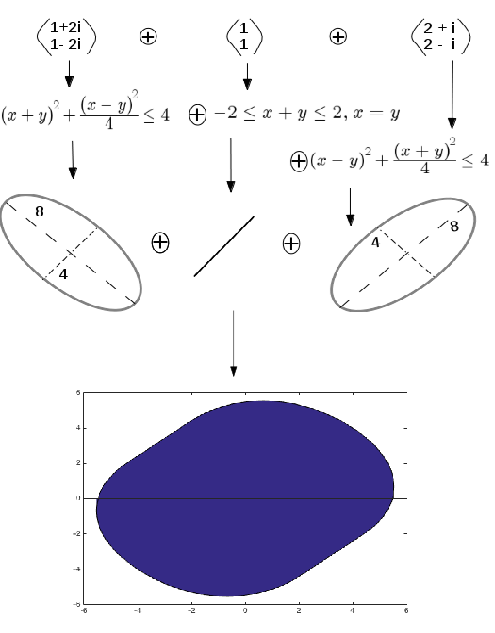
\includegraphics[scale=0.43]{fig/cznew.png}\\[1em]
%% 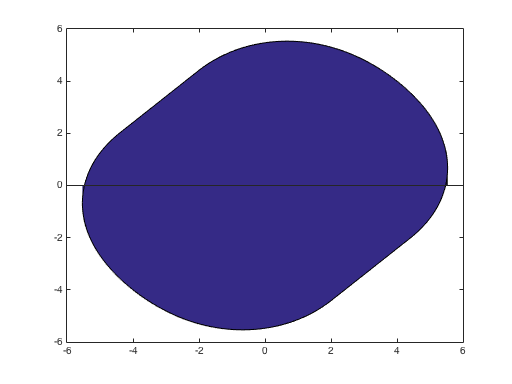
\includegraphics[scale=0.5]{fig/CZhull.png}
%% \caption{Real projection of a complex zonotope as\\ Minkowski sum of 2 ellipses and 1 line segment }~\label{fig:cz}
%% \end{figure}
%% %

As the real projection of the generator of a complex zonotope can
either be an ellipsoid or a line segment, a complex zonotope can
represent a Minkowski sum of line segments as well as some
ellipsoids.  The non-polyhedral real projections along the three axis
oriented hyperplanes of the following 3-D complex zonotope is shown in
Figure~\ref{fig:3dcztope}
%
\[
\cztope{\mymatrix{-0.2226  & -0.1335 + 0.1769\iota  & -0.1335 - 0.1769\iota\\
   0.3615 &   0.2713 + 0.3991\iota &  0.2713 - 0.3991\iota\\
   0.2446 &  -0.8473 &  -0.8473}}{0}
\]
%
\begin{figure}
\center
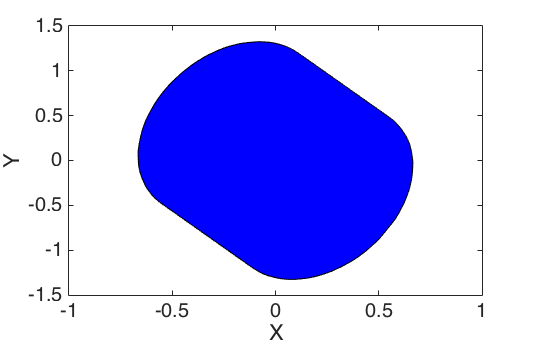
\includegraphics[scale=0.5]{fig/CZtopes/xycz.png}
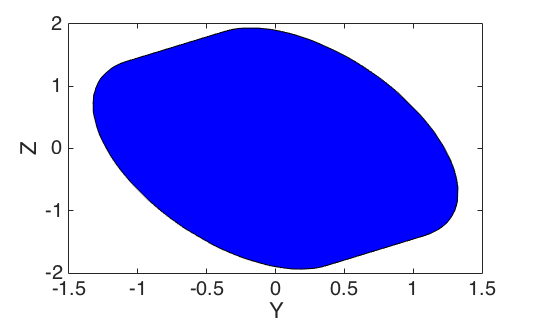
\includegraphics[scale=0.5]{fig/CZtopes/yzcz.png}
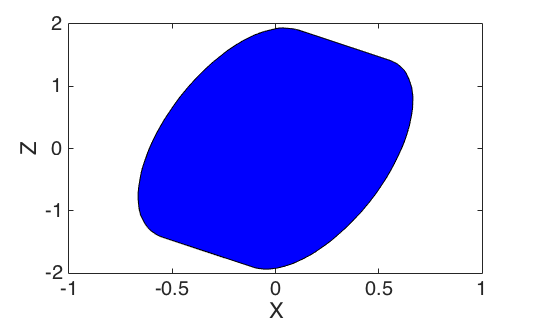
\includegraphics[scale=0.5]{fig/CZtopes/xzcz.png}
\caption{Real projection of complex zonotope on axis oriented hyperplanes}~\label{fig:3dcztope}
\end{figure}
%

\emph{Contraction along eigenvectors:  }  A motivation for extending
simple zonotopes to complex zonotopes is that a complex zonotope with
its generators as the complex eigenvectors of a discrete time linear
system is positively invariant if the complex eigenvalues
corresponding to the generators are bounded within unity in their
absolute values.  This is because the generators of the resultant
complex zonotope after transformation will be scaled by the absolute
values of the corresponding eigenvalues.  For example, consider the
following matrix $A$ and the complex zonotope
$\cztope{V}{0}$ generated by the complex eigenvectors of $A$.
%
\begin{align*}
& A=\mymatrix{
0.1502 &  -0.0438  &  0.1366\\
    0.7482 &   0.1470  &  0.1251\\
   -0.8436 &  -0.7027  &  0.0418
}\\
& V=\mymatrix{
-0.2226  &  -0.1335 + 0.1769\iota &  -0.1335 - 0.1769\iota\\
   0.3615 &   0.2713 + 0.3991\iota &  0.2713 - 0.3991\iota\\
   0.2446 & -0.8473 &   -0.8473 
}
\end{align*}
%
The eigenvalues of $A$ are $-0.2291$, $0.1339 + 0.5071\iota$ and
${0.1339 - 0.5071\iota}$, whose absolute values are $0.2291$,
$0.5245$, and $0.5245$, respectively.  After the transformation by
$A$, the set generated by $V^T_1$ gets scaled down to $0.2291$ times
its size and that of $V^T_2$ and $V^T_3$ to $0.5245$ times
its their size.  So, the complex zonotope, which is a Minkowski sum
of these sets, contracts after the transformation.  This is illustrated
in Figure~\ref{fig:cz-scaled-down}, which shows the contraction of
each of the sets formed by the generators and the consequent
contraction of the complex zonotope.
%
\begin{figure}
\center
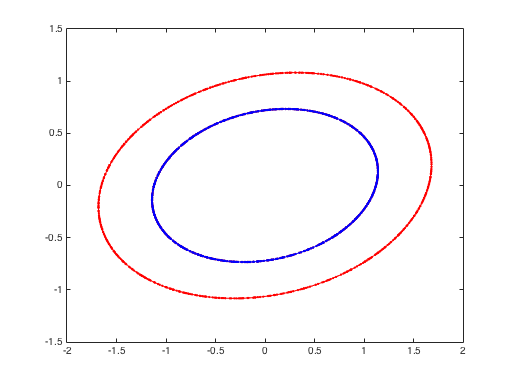
\includegraphics[scale=0.4]{fig/CZtopes/eigcontraction.png}
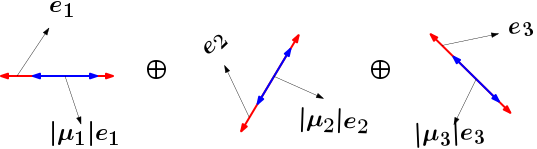
\includegraphics[scale=0.5]{fig/CZtopes/contraction-zonotope.png}
\caption{Contraction of complex zonotope along
eigenvectors}~\label{fig:cz-scaled-down}
\end{figure}
%
This property of contraction of complex zonotope by a linear
transformation based on the eigenstructure of a matrix is explained
mathematically in the following proposition.
%
\begin{proposition}[Eigenstructure based invariance]~\label{lem:eig-invariance}
Let us consider $\ptemp\in\mat{n}{n}{\compnums}$ consists of the
complex eigenvectors of a matrix $A\in\mat{n}{n}{\reals}$ as its
column vectors and $\mu\in\compnums^n$ be the vector of complex
eigenvalues, i.e., $A\ptemp = \ptemp\diagonal{\mu}$.
Then \[A\lt(\cztope{\ptemp}{0}\rt)
= \cztope{\ptemp\diagonal{{\mu}}}{0}.\]  If
$\infnorm{\mu}\leq 1$, then
$A\lt(\rztope{\ptemp}{0}\rt)\subseteq \rztope{\ptemp}{0}$.
\end{proposition}
% 
\begin{proof}
We derive
  %
\begin{align*}
& A\lt(\cztope{\ptemp}{0}\rt) =
A\set{\ptemp\zeta:~\zeta\in\compnums^n,\infnorm{\zeta}\leq 1}\\
& =\set{A\ptemp\zeta:~\zeta\in\compnums^n,\infnorm{\zeta}\leq 1}
= \cztope{A\ptemp}{0}=\cztope{\ptemp\diagonal{\mu}}{0}.
\end{align*}
%
which proves the first part of the
Proposition.

For the second part, we are given that $\infnorm{\mu}\leq 1$.
Consider a point
%
\begin{align*}
  & y\in A\cztope{\ptemp}{0}=\cztope{\ptemp\diagonal{\mu}}{0}~~\text{where}\\
  &y = \ptemp\diagonal{\mu}\delta:\infnorm{\delta}\leq
1.
\end{align*}
%
Let $\zeta = \diagonal{\mu}\delta$. Then $\infnorm{\zeta} \leq
\infnorm{\mu}\infnorm{\delta} \leq 1$.  So,
%
\begin{align*}
  & y=\ptemp\zeta~~\text{ where }~
  \infnorm{\zeta}\leq 1.
\end{align*}
%
So, we get $y\in \cztope{\ptemp}{0}$.  As this is true for all
$y\in\cztope{\ptemp}{0}$, we have
$A\lt(\cztope{\ptemp}{0}\rt)\subseteq
\cztope{\ptemp}{0}$ when $\infnorm{\mu}\leq 1$.
\end{proof}
%If we add more generators to the above representation of a complex
zonotope, it would increase the size of the complex zonotope.
Therefore, we can not find better approximations of a given set by
only adding more generators to the complex zonotope.  Moreover, adding
a generator can violate positive invariance.  For example, consider
the complex zonotope $\cztope{\ptemp}{0}$, where
%
\[
\ptemp = \mymatrix{-0.2226 &  -0.1335 + 0.1769\iota &   -0.1335 - 0.1769\iota\\
   0.3615  &   0.2713 + 0.3991\iota &   0.2713 - 0.3991\iota\\
   0.2446  &   -0.8473 &  -0.8473}.
\]
%
The above complex zonotope contracts after transformation by the matrix
%
\[
A = \mymatrix{-0.2766 &   -0.0806 &    0.2516\\
    1.3779  &  0.2707  &   0.2304\\
   -1.5536 &  -1.2942 &    0.0769}
\]
%
as shown in Figure~\ref{fig:refinement}.  On the other hand, when we
add another generator $\mymatrix{0 & 0.5 & 0.5}^T$, then the complex
zonotope, $\cztope{W}{0}$, where
%
\[
W=\mymatrix{-0.2226 &  -0.1335 + 0.1769\iota &   -0.1335 -
   0.1769\iota & 0\\
   0.3615 &   0.2713 + 0.3991\iota &   0.2713 -
   0.3991\iota & 0.5\\
   0.2446 &   -0.8473 + 0.0000\iota &  -0.8473 & 0.5}
\]
%
does not contract as illustrated in Figure~\ref{fig:refinement}.
%
\begin{figure}
\center
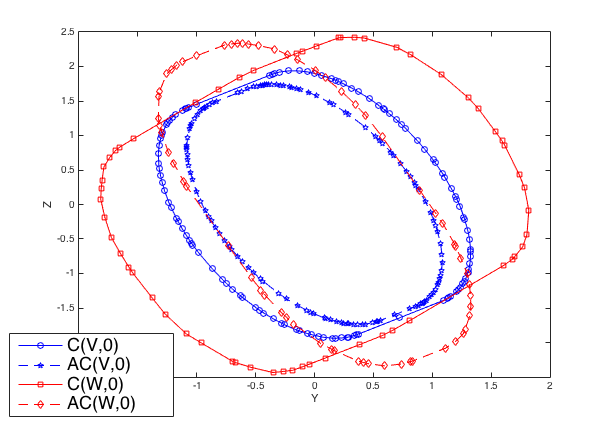
\includegraphics[scale=0.5]{fig/CZtopes/refinement.png}
\caption{Violation of positive invariance and size increase after
adding a generator to the basic representation.}~\label{fig:refinement}
\end{figure}

Alternatively, to refine
a complex zonotope, we can adjust the magnitude of contribution of
each generator to the size of the set while also preserving the
positive invariance.  This way, can also add more generators and
increase approximation accuracy by adjusting the magnitudes of each
generator.  In order to conveniently perform algebraic manipulations
on the magnitude of each generator, we can explicitly specify variable
bounds on the combining coefficients.  This gives us a more general
representation, which we call as {\it template complex zonotope},
where the magnitude of each combining coefficient is bounded in its
absolute value a {\it scaling factor}.  We call the matrix whose
column vectors generate a template complex zonotope as a {\it
template}.  This representation is similar in spirit to the known
template based set
representations~\cite{Sankaranarayanan+Dang+Ivancic-08-Symbolic,DBLP:journals/lisp/Mine06}
in abstract interpretation, where for some fixed template, subsets of
metric spaces are mapped to points in a lattice.  In the case of a
template complex zonotope, for a fixed template, subsets of the
complex vector space can be mapped to the {\it scaling factors}.
%
\begin{definition}[Template complex zonotope]
Let us consider ${\ptemp\in\mat{n}{m}{\compnums}}$ called the template,
${\sfact\in\reals^m_{\geq 0}}$ called scaling factors and
${\cen\in\compnums^n}$ called the center.  Then the following is a template
complex zonotope.
%
\begin{equation}
\tcztope{\ptemp}{\cen}{\sfact}
= \set{\ptemp\zeta+\cen:~\absolute{\zeta_i}\leq \sfact_i~\forall
i\in\set{1,...,m}}.
\end{equation}
\end{definition}
In further discussion, we use the term {\it representation size} of a
template complex zonotope to refer to the size of the template matrix.
In the rest of this chapter, we consider the following notation,
unless otherwise specified.
%
\[
\ptemp\in\mat{n}{m}{\compnums},~~\cen\in\compnums^n,~~\sfact\in\reals^m_{\geq 0}.
\]
%
A template complex zonotope can be converted to the basic
representation of the complex zonotope by multiplying the diagonal
matrix of scaling factors to the template.  This is described in the
following lemma.
%
\begin{lemma}[Normalization]~\label{lem:normalization}
Let us consider ${\mu\in\compnums^m}$.
%
\begin{align*}
\text{Then}\hspace{3em}&\tcztope{\ptemp\diagonal{\mu}}{\cen}{\sfact}=\tcztope{\ptemp}{\cen}{\diagonal{\absolute{\mu}}\sfact}.~\numberthis\label{eqn:normalization}\\
\text{Therefore},\hspace{3em} & \tcztope{\ptemp}{\cen}{\sfact}=\cztope{\ptemp\diagonal{\sfact}}{\cen}.
\end{align*}
%
\end{lemma}
%
\begin{proof}
Consider a point $x\in\tcztope{\ptemp\diagonal{\mu}}{\cen}{\sfact}$,
where
%
\[
x=\cen+\ptemp\diagonal{\mu}\zeta:\absolute{\zeta}\leq\sfact.
\]
%
Let $\zeta^\pr=\diagonal{\mu}\zeta$.  Then, $x=c+\ptemp\zeta^\pr$.
We get
%
\[
\absolute{\zeta^\pr}=\diagonal{\absolute{\mu}}\absolute{\zeta}\leq\diagonal{\absolute{\mu}}\sfact.
\]

Therefore, ${x\in\tcztope{\ptemp}{\cen}{\diagonal{\mu}\sfact}}$.  This
means,
%
\[
\tcztope{\ptemp\diagonal{\mu}}{\cen}{\sfact}\subseteq\tcztope{\ptemp}{\cen}{\diagonal{\absolute{\mu}}\sfact}
\]
%
Next consider a point
$y\in\tcztope{\ptemp}{\cen}{\diagonal{\absolute{\mu}\sfact}}$ where
%
\[
y=\cen+\ptemp\epsilon:~\absolute{\epsilon}\leq
\diagonal{\absolute{\mu}}\sfact.
\]
%
Let us consider $\epsilon^\pr\in\compnums^m$, such that
%
\[\forall i\in\set{1,...,m},~~
\epsilon_i=\left\{
\begin{array}{l}
\frac{\epsilon_i}{\mu_i}~\text{if}~\mu_i\neq 0\\
0~\text{if}~\mu_i=0.
\end{array}
\right.
\]
%
We shall show that $\epsilon=\epsilon^\pr\diagonal{\mu}$, i.e., for
any $i\in\set{1,...,m}$, $\epsilon_i=\epsilon^\pr_i\mu_i$.  We prove
it in the following two cases.
\begin{enumerate}
\item Let us consider $\epsilon_i\neq 0$.  As
$\absolute{\epsilon}\leq\absolute{\diagonal{\mu_i}}\sfact$, so
  $\mu_i\neq 0$.  Therefore,
  \[
  \epsilon_i=\frac{\epsilon_i}{\mu_i}\mu_i=\epsilon^\pr_i\mu_i.
  \]
\item Let us consider $\epsilon_i=0$.  As
$\absolute{\epsilon}\leq\absolute{\diagonal{\mu_i}}\sfact$, so $\mu_i=
  0$.  This implies
  \[
  0=\epsilon=\epsilon^\pr_i\times
  0=\epsilon^\pr_i\mu_i.
  \]
  %
\end{enumerate}
%
So, we get $y=\cen+\ptemp\diagonal{\mu_i}\epsilon^\pr$.  By the definition of
$\epsilon^\pr$, we get
%
\[\forall i\in\set{1,...,m}~~
\absolute{\epsilon^\pr_i}\leq
\left\{
\begin{array}{l}
\absolute{\frac{\epsilon_i}{\mu_i}}\leq\frac{\absolute{\mu_i}\sfact_i}{\absolute{\mu_i}}=\sfact_i~\text{if}~\mu_i\neq
0\\
0~\text{if}~\mu_i=0
\end{array}
\right.
\]
%
Therefore, $\absolute{\epsilon^\pr}\leq\sfact$.  So,
$y\in\tcztope{\ptemp\diagonal{\mu}}{\cen}{\sfact}$.  Therefore,
%
\[
\tcztope{\ptemp}{\cen}{\diagonal{\absolute{\mu}}\sfact}\subseteq\tcztope{\ptemp\diagonal{\mu}}{\cen}{\sfact}.
\]
%
Combining the previous two conclusions, we get
Equation~\ref{eqn:normalization}.

By definition,
%
\begin{align*}
& \cztope{\ptemp\diagonal{\sfact}}{\cen}=\tcztope{\ptemp\diagonal{\sfact}}{\cen}{\repmat{1}{m}{1}}\\
& \%\%~~\text{by Equation~\ref{eqn:normalization}}\\
& =\tcztope{\ptemp}{\cen}{\diagonal{{\sfact}}\repmat{1}{m}{1}}=\tcz{\ptemp}{\cen}{\sfact}.~\hspace{3em}\qedhere
\end{align*}
%
\end{proof}
%


\section{Basic operations}
We shall now describe other operations on augmented complex zonotopes
like are linear transformation, Minkowski sum, support function and
checking inclusion.

Augmented complex zonotopes are closed under linear transformation and
Minkowski sum, as described in the following two lemmas.  This
is because an augmented complex is specified as a Minkowski sum of a template
complex zonotope and an interval zonotope, both of which are closed
under these operations.
%
\begin{lemma}[Linear transformation]
Let us consider $A\in\mat{n}{n}{\reals}$.  Then
%
\[
A\acztope{\ptemp}{\cen}{\sfact}{\stemp}{\lb}{\ub}=\acztope{A\ptemp}{A\cen}{\sfact}{A\stemp}{\lb}{\ub}.
\]
%
\end{lemma}
%
\begin{proof}
  We derive the following.
  %
  \begin{align*}
    & A\acztope{\ptemp}{\cen}{\sfact}{\stemp}{\lb}{\ub}=
    A\lt(\minsum{\tcztope{\ptemp}{\cen}{\sfact}}{\iztope{\stemp}{\lb}{\ub}}\rt)\\
    & \%\%~\text{by Lemmas~\ref{lem:lin-transform} and~\ref{lem:iz-lin-transform}}\\
    &
    = \minsum{\tcztope{A\ptemp}{A\cen}{\sfact}}{\iztope{A\stemp}{\lb}{\ub}}\\
    & = \acztope{A\ptemp}{A\cen}{\sfact}{A\stemp}{\lb}{\ub}.~~~~~~~~~~~~~\qedhere
  \end{align*}
  %
\end{proof}
%
\begin{lemma}[Minkowski sum]
The following is true.
%
\begin{align*}
& \minsum{\acztope{\ptemp}{\cen}{\sfact}{\stemp}{\lb}{\ub}}
  {\acztope{\ptemp^\pr}{\cen^\pr}{\sfact^\pr}{\stemp^\pr}{\lb^\pr}{\ub^\pr}}\\
& = \acztope
{\lt[\begin{matrix}
    \ptemp &
    \ptemp^\pr
  \end{matrix}\rt]
}
{\begin{matrix}
    \cen+\cen^\pr
  \end{matrix}
}
{\lt[\begin{matrix}
    \sfact\\
    \sfact^\pr
  \end{matrix}\rt]
}
{\lt[\begin{matrix}
    \stemp &
    \stemp^\pr
  \end{matrix}\rt]
}
{\lt[\begin{matrix}
    \lb\\
    \lb^\pr
  \end{matrix}\rt]
}
{\lt[\begin{matrix}
    \ub\\
    \ub^\pr
  \end{matrix}\rt]
}
\end{align*}
%
\end{lemma}
%
\begin{proof}
  We derive the following.
  %
  \begin{align*}
& \minsum{\acztope{\ptemp}{\cen}{\sfact}{\stemp}{\lb}{\ub}}
    {\acztope{\ptemp^\pr}{\cen^\pr}{\sfact^\pr}{\stemp^\pr}{\lb^\pr}{\ub^\pr}}\\
& =
    \minsum{\tcztope{\ptemp}{\cen}{\sfact}}{\iztope{\stemp}{\lb}{\ub}}
    \oplus\minsum{\tcztope{\ptemp^\pr}{\cen^\pr}{\sfact^\pr}}{\iztope{\stemp^\pr}{\lb^\pr}{\ub^\pr}}\\
&
    =\lt(\minsum{\tcztope{\ptemp}{\cen}{\sfact}}{\tcztope{\ptemp^\pr}{\cen^\pr}{\sfact^\pr}}\rt)
    \oplus\lt(\minsum{\iztope{\stemp}{\lb}{\ub}}{\iztope{\stemp^\pr}{\lb^\pr}{\ub^\pr}}\rt)\\
    & \%\%~\text{by Lemmas~\ref{lem:min-sum} and~\ref{lem:iz-min-sum}}\\
& = \minsum{\tcztope{\begin{bmatrix}\ptemp &
          \ptemp^\pr\end{bmatrix}}{\cen+\cen^\pr}{\begin{bmatrix}\sfact\\\sfact^\pr\end{bmatrix}}}
             {\iztope{\mymatrix{\stemp &
                   \stemp^\pr}}{\mymatrix{\lb\\\lb^\pr}}{\mymatrix{\ub\\\ub^\pr}}}\\
& =  \acztope
{\lt[\begin{matrix}
    \ptemp &
    \ptemp^\pr
  \end{matrix}\rt]
}
{\begin{matrix}
    \cen+\cen^\pr
  \end{matrix}
}
{\lt[\begin{matrix}
    \sfact\\
    \sfact^\pr
  \end{matrix}\rt]
}
{\lt[\begin{matrix}
    \stemp &
    \stemp^\pr
  \end{matrix}\rt]
}
{\lt[\begin{matrix}
    \lb\\
    \lb^\pr
  \end{matrix}\rt]
}
{\lt[\begin{matrix}
    \ub\\
    \ub^\pr
  \end{matrix}\rt]
}.~~~~~~~~~~~~~~~~~~~\qedhere            
    \end{align*}
%
\end{proof}
%
To problem of checking inclusion between two augmented complex
zonotopes can be equivalently expressed as the problem of checking
inclusion between two geometrically equivalent template complex
zonotopes.  For this, we use the following equivalence between the
real projections of an augmented complex zonotope and a template
complex zonotope.
%
\begin{lemma}~\label{lem:acz-tcz-conversion}
The following is true.
%
\begin{align*}
  \real\lt(\acztope{\ptemp}{\cen}{\sfact}{\stemp}{\lb}{\ub}\rt)
  = \real\lt(\tcztope
  {\lt[\begin{matrix}
      \ptemp &
      \stemp
    \end{matrix}\rt]
  }
  {\begin{matrix}
      \cen+\frac{\ub+\lb}{2}
    \end{matrix}
  }
  {\lt[\begin{matrix}
      \sfact\\
      \frac{\ub-\lb}{2}
    \end{matrix}\rt]
  }
  \rt).
\end{align*}
%
\end{lemma}
%
\begin{proof}
  We derive the following.
  %
  \begin{align*}
    & \real\lt(\acztope{\ptemp}{\cen}{\sfact}{\stemp}{\lb}{\ub}\rt)
    =
    \real\lt(\tcztope{\ptemp}{\cen}{\sfact}\rt)\oplus\iztope{\stemp}{\lb}{\ub}\\
    & \%\%~\text{By Lemma~\ref{lem:iz-tcz-conversion}}\\
    & =
    \real\lt(\tcztope{\ptemp}{\cen}{\sfact}\rt)\oplus\real\lt(\tcztope{\stemp}{\stemp\frac{\ub+\lb}{2}}{\frac{\ub-\lb}{2}}\rt)\\
    &
  = \real\lt(\tcztope
  {\lt[\begin{matrix}
      \ptemp &
      \stemp
    \end{matrix}\rt]
  }
  {\begin{matrix}
      \cen+\frac{\ub+\lb}{2}
    \end{matrix}
  }
  {\lt[\begin{matrix}
      \sfact\\
      \frac{\ub-\lb}{2}
    \end{matrix}\rt]
  }
  \rt).\hspace{4em}\qedhere
   \end{align*}
  %
\end{proof}
%
 In Definition~\ref{defn:inclusion-tcz} of the previous chapter, we
 introduced a partial order ``$\order$'', as a sufficient convex
 condition for checking inclusion between two template complex
 zonotopes.  We extend the relation for checking inclusion between two
 augmented complex zonotopes as follows.
%
\begin{definition}[Ordering between augmented complex zonotopes]~\label{defn:inclusion-acz}
We say that
%
\begin{align*}
& \acztope{\ptemp^\pr}{\cen^\pr}{\sfact^\pr}{\stemp^\pr}{\lb^\pr}{\ub^\pr} \order
 \acztope{\ptemp}{\cen}{\sfact}{\stemp}{\lb}{\ub}~~\text{iff}\\
& \tcztope
  {\lt[\begin{matrix}
      \ptemp^\pr &
      \stemp^\pr
    \end{matrix}\rt]
  }
  {\begin{matrix}
      \cen^\pr+\frac{\ub^\pr+\lb^\pr}{2}
    \end{matrix}
  }
  {\lt[\begin{matrix}
      \sfact^\pr\\
      \frac{\ub^\pr-\lb^\pr}{2}
    \end{matrix}\rt]
  }  
  \order
  \tcztope
  {\lt[\begin{matrix}
      \ptemp &
      \stemp
    \end{matrix}\rt]
  }
  {\begin{matrix}
      \cen+\frac{\ub+\lb}{2}
    \end{matrix}
  }
  {\lt[\begin{matrix}
      \sfact\\
      \frac{\ub-\lb}{2}
    \end{matrix}\rt]
  }.~\numberthis\label{eqn:order-acz}
\end{align*}
%
\end{definition}
%
\begin{theorem}[Inclusion-checking and partial order]~\label{thm:acz-inclusion}
All of the following is true.
\begin{enumerate}
  \item Sufficient condition for inclusion:
%
    \begin{align*}
& \acztope{\ptemp^\pr}{\cen^\pr}{\sfact^\pr}{\stemp^\pr}{\lb^\pr}{\ub^\pr}\order\acztope{\ptemp}{\cen}{\sfact}{\stemp}{\lb}{\ub}\\    
&\implies \real\lt(\acztope{\ptemp^\pr}{\cen^\pr}{\sfact^\pr}{\stemp^\pr}{\lb^\pr}{\ub^\pr}\rt)\subseteq\real\lt(\acztope{\ptemp}{\cen}{\sfact}{\stemp}{\lb}{\ub}\rt).
\end{align*}
%
\item The relation ``$\order$'' is a partial order on
  augmented complex zonotopes.
\end{enumerate}
%
\end{theorem}
%
\begin{proof}
  We derive the following.
  %
  \begin{align*}
&    \acztope{\ptemp^\pr}{\cen^\pr}{\sfact^\pr}{\stemp^\pr}{\lb^\pr}{\ub^\pr}\order\acztope{\ptemp}{\cen}{\sfact}{\stemp}{\lb}{\ub}\\
& \equivalent   \tcztope
  {\lt[\begin{matrix}
      \ptemp^\pr &
      \stemp^\pr
    \end{matrix}\rt]
  }
  {\begin{matrix}
      \cen^\pr+\frac{\ub^\pr+\lb^\pr}{2}
    \end{matrix}
  }
  {\lt[\begin{matrix}
      \sfact^\pr\\
      \frac{\ub^\pr-\lb^\pr}{2}
    \end{matrix}\rt]
  }  
  \order
  \tcztope
  {\lt[\begin{matrix}
      \ptemp &
      \stemp
    \end{matrix}\rt]
  }
  {\begin{matrix}
      \cen+\frac{\ub+\lb}{2}
    \end{matrix}
  }
  {\lt[\begin{matrix}
      \sfact\\
      \frac{\ub-\lb}{2}
    \end{matrix}\rt]
  }\\
  & \%\%~~\text{By Theorem~\ref{thm:suff-inclusion}}\\
  & \implies
  \tcztope
  {\lt[\begin{matrix}
      \ptemp^\pr &
      \stemp^\pr
    \end{matrix}\rt]
  }
  {\begin{matrix}
      \cen^\pr+\frac{\ub^\pr+\lb^\pr}{2}
    \end{matrix}
  }
  {\lt[\begin{matrix}
      \sfact^\pr\\
      \frac{\ub^\pr-\lb^\pr}{2}
    \end{matrix}\rt]
  }  
  \subseteq
  \tcztope
  {\lt[\begin{matrix}
      \ptemp &
      \stemp
    \end{matrix}\rt]
  }
  {\begin{matrix}
      \cen+\frac{\ub+\lb}{2}
    \end{matrix}
  }
  {\lt[\begin{matrix}
      \sfact\\
      \frac{\ub-\lb}{2}
    \end{matrix}\rt]
  }\\
  & \%\%~~\text{By Lemma~\ref{lem:acz-tcz-conversion}}\\
&\implies
  \real\lt(\acztope{\ptemp^\pr}{\cen^\pr}{\sfact^\pr}{\stemp^\pr}{\lb^\pr}{\ub^\pr}\rt)\subseteq\real\lt(\acztope{\ptemp}{\cen}{\sfact}{\stemp}{\lb}{\ub}\rt).
  \end{align*}
  %
Since ``$\order$'' is a partial order on template complex zonotopes,
Equation~\ref{eqn:order-acz} implies that it is also a partial order on augmented
complex zonotopes.
\end{proof}
%
\begin{remark}
We have explained for template complex zonotopes that the relation
``$\order$'' is equivalent to second order conic constraints on the
center, scaling factors and some auxillary variables.  Therefore,
according to Equation~\ref{eqn:order-acz}, the extension of ``$\order$''
to augmented complex zonotopes is equivalent to second order conic
constraints on the primary offset, scaling factors, lower and upper
interval bounds and some auxillary variables.
\end{remark}
%
The support function of an augmented complex zonotope is as an affine
expression of the primary offset, scaling factors and the upper and
lower interval bounds.  This is described in the following lemma.
%
\begin{lemma}[Support function]~\label{lem:support-acz}
Let us consider
$v\in\reals^n$.  Then
%
\begin{align*}
  & \supp{v}{\real\lt(\acztope{\ptemp}{\cen}{\sfact}{\stemp}{\lb}{\ub}\rt)}\\
  & = \real\lt(v^T\mymatrix{\ptemp &
    \stemp}\lt(\cen+\frac{\ub+\lb}{2}\rt)\rt)+\absolute{v^T\mymatrix{\ptemp & \stemp}}\mymatrix{\sfact\\\frac{\ub-\lb}{2}}.
\end{align*}
%
\end{lemma}
%
\begin{proof}
  We derive the following:
  %
  \begin{align*}
& \%\%~~\text{by Lemma~\ref{lem:acz-tcz-conversion}}\\
&
    \supp{v}{\real\lt(\acztope{\ptemp}{\cen}{\sfact}{\stemp}{\lb}{\ub}\rt)}\\
& = \supp{v}{\real\lt(\tcztope
  {\lt[\begin{matrix}
      \ptemp &
      \stemp
    \end{matrix}\rt]
  }
  {\begin{matrix}
      \cen+\frac{\ub+\lb}{2}
    \end{matrix}
  }
  {\lt[\begin{matrix}
      \sfact\\
      \frac{\ub-\lb}{2}
    \end{matrix}\rt]
  }
  \rt)}\\
    & \%\%~\text{by Lemma~\ref{lem:support-tcz}}\\
    & =\real\lt(v^T\mymatrix{\ptemp &
    \stemp}\lt(\cen+\frac{\ub+\lb}{2}\rt)\rt)+\absolute{v^T\mymatrix{\ptemp & \stemp}}\mymatrix{\sfact\\\frac{\ub-\lb}{2}}.~\hspace{2em}\qedhere
  \end{align*}
  %
\end{proof}
%




\section{Checking inclusion}
While computing positive invariants using a set representation,
ascertaining the positive invariance of a set requires deciding the
inclusion of the next reachable set inside the given set.  In the case
of complex zonotopes, we shall show that checking the exact inclusion
amounts to solving a is a non-convex optimization problem.  Therefore,
we later find a sufficient condition expressed by convex constraints
for checking the inclusion.  The convex constraints we derive later
are specifically second order conic constraints, which are described
below.
%
\begin{definition}[Second order conic constraint]
A second order conic constraint on a variable $x$ taking values in
$\reals^n$ is one of the following expressions.
\begin{enumerate}
\item $\sqnorm{Ax+b}\leq c^Tx+d$ where $A\in\mat{r}{n}{\reals}$,
  $b\in\reals^r$, $c\in\reals^n$ and $d\in\reals$.
\item $p^Tx=q$ where $p\in\reals^n$ and $q\in\reals$.
\end{enumerate}
\end{definition}
%
\begin{example}
%
An inequality like $x^2+4y^2+25z^2-3x-4y+z+3\leq 0$ is a second order
  conic constraint because it can be written as
%
\[
\norm{\mymatrix{
    1 & 0 & 0\\
    0 & 2 & 0\\
    0 & 0 & 5
}\mymatrix{x\\y\\z}}\leq \mymatrix{3 & 4 & -1}\mymatrix{x\\y\\z}+2.
\]
A linear equality like $3x+2y-4z=5$ is also a second order conic
constraint.
\end{example}
%
In the case of complex zonotope, we shall later derive a set of second
order conic constraints, which have to be collectively satisfied to
guarantee inclusion.  Given a set of second order conic constraints on
a variable $x\in\reals^n$, solving the constraints refers to finding a
value $x^*\in\reals^n$ that satisfies the constraints.  A value
$x^\pr\in\reals^n$ is called an approximate solution within a
precision $\epsilon\in\reals_{\geq 0}$ if there exists a solution
$x^*\in\reals^n$ such that $\sqnorm{x^\pr-x^*}\leq \epsilon$.  There
are tools based on interior point methods (see~\cite{grant2008cvx})
that can efficiently find approximate solutions with very high
precision to second order conic constraints (SOCC).

Checking inclusion of a single point inside a template complex
zonotope is equivalent to solving SOCC, as described below.
%
\begin{lemma}[Inclusion of a point]
Let us consider a point $x\in\compnums^n$.  Then
$x\in\tcztope{\ptemp}{\cen}{\sfact}\subset\compnums^n$ if and only if
all of the following is collectively true.
%
\begin{align}
& \exists\zeta\in\compnums^m:\nonumber\\
& \ptemp\zeta = x-c~\label{eqn:lem-point-inclusion-1}\\
& \absolute{\zeta}\leq \sfact.~\label{eqn:lem-point-inclusion-2}
\end{align}
%
\end{lemma}
%
\begin{proof}
The above result follows from the fact that any point 
$x\in\tcztope{\ptemp}{\cen}{\sfact}$ is of the form
$x=\cen+\ptemp\zeta$ for some $\zeta\in\compnums^m$ such that
$\absolute{\zeta}\leq \sfact$.
\end{proof}
%
\begin{example}
Let us consider the template complex zonotope
$\tcztope{\ptemp}{\cen}{\sfact}\subset\compnums^2$ and a point $x\in\compnums^2$,
where
%
\[
\ptemp=\mymatrix{1+\iota & 1 & 0\\1 & 0 & 1},~~\cen = \mymatrix{\iota\\ 1},~~\sfact=\mymatrix{1\\1\\1}~\text{and}~x=\mymatrix{2\iota-2\\\iota+2}.
\]
%
To prove that $x\in\tcztope{\ptemp}{\cen}{\sfact}$, let us consider
$\zeta=\mymatrix{\iota & -1 & 1}^T$.  Then we get
%
\[
\ptemp\zeta = \mymatrix{\iota-2\\\iota+1}= \mymatrix{2\iota-2\\\iota+2}-\mymatrix{\iota\\1}=x-c.
\]
%
Therefore, Equation~\ref{eqn:lem-point-inclusion-1} is satisfied.  Furthermore,
$\absolute{\zeta}=\mymatrix{1 & 1 & 1}^T$.  So, Equation~\ref{eqn:lem-point-inclusion-2} is
also satisfied.  Henceforth, $x\in\tcztope{\ptemp}{\cen}{\sfact}$.
\end{example}
%
Equation~\ref{eqn:lem-point-inclusion-1} is an equality constraint on
$\zeta$, which is therefore an SOCC.  We know that the absolute value
of a complex number is the square norm of a two dimensional vector.
So, Equation~\ref{eqn:lem-point-inclusion-2} is equivalent to a set of
square norm constraints on the real and imaginary components of
$\zeta$, which are therefore SOCC constraints.  Hence, the inclusion
of a point inside a template complex zonotope can be checked by
solving second order conic constraints.

Now we state the necessary and sufficient condition for checking
inclusion between two template complex zonotopes.
%
\begin{lemma}[Exact inclusion between template complex zonotopes]~\label{lem:exact-inclusion}
Let us consider $\ptemp\in\mat{n}{m}{\compnums}$ and
$\ptemp^\pr\in\mat{n}{r}{\compnums}$.  The inclusion
$\tcztope{\ptemp^\pr}{\cen^\pr}{\sfact^\pr}\subseteq\tcztope{\ptemp}{\cen}{\sfact}$
holds if and only if
\begin{equation}\label{eqn:exact-inclusion}
\max_{\set{\zeta^\pr\in\compnums^{r}:\absolute{\zeta^\pr}\leq \sfact^\pr}}\min_{\set{\zeta\in\compnums^m:\ptemp\zeta=\ptemp^\pr\zeta^\pr+\cen^\pr-\cen}}\max_{i=1}^m\lt(\absolute{\zeta_i}-s_i\rt)\leq 0
\end{equation}
\end{lemma}
%
\begin{proof}
  We have
  %
  \begin{align*}
    &\tcztope{\ptemp}{\cen}{\sfact}=\set{\cen+\ptemp\zeta:~\zeta\in\compnums^m,~\absolute{\zeta}\leq\sfact},\\
    &\tcztope{\ptemp^\pr}{\cen^\pr}{\sfact^\pr}=\set{\cen^\pr+\ptemp^\pr\zeta^\pr:~\zeta^\pr\in\compnums^r,~\absolute{\zeta^\pr}\leq\sfact^\pr}.
  \end{align*}
  %
Therefore, we get
$\tcztope{\ptemp^\pr}{\cen^\pr}{\sfact^\pr}\subseteq\tcztope{\ptemp}{\cen}{\sfact}$
if and only if
for every $\zeta^\pr\in\compnums^r:\absolute{\zeta^\pr}\leq \sfact^\pr$,
there exists
$\zeta\in\compnums^m:\ptemp\zeta+\cen=\ptemp^\pr\zeta^\pr+\cen^\pr~\wedge~\absolute{\zeta}\leq
\sfact$.  This is equivalently expressed as the constraint in Equation~\ref{eqn:exact-inclusion}.
\end{proof}
%
The reason solving Equation~\ref{eqn:exact-inclusion}
requires non-convex optimization is explained as follows.  Let us consider
that $\ptemp$ has a pseudo-inverse $\pinv{\ptemp}$.  Then by the
rank-nullity theorem
%
\[
\set{\zeta:~\ptemp\zeta=\ptemp\zeta^\pr+\cen^\pr-\cen}=\set{\pinv{\ptemp}\lt(\zeta^\pr-c\rt)+v:~v\in\nullspace{\ptemp}}
\]
%
So,
%
\begin{align*}
& \min_{\set{\zeta\in\compnums:\ptemp\zeta=\ptemp^\pr\zeta^\pr+\cen^\pr-\cen}}\max_{i=1}^m\lt(\absolute{\zeta_i}-s_i\rt)\\
&
=\min_{\set{v\in\nullspace{\ptemp}}}\max_{i=1}^m\lt(\absolute{\pinv{\ptemp}\lt(\zeta^\pr-c\rt)+v}-s_i\rt)
\end{align*}
%
The absolute value of a complex variable is a convex quadratic
function of the real and imaginary components of the variable.  So,
the above function is a point-wise minimum (for points $v$ in the null
space $\null{\ptemp}$) of a set of convex quadratic functions over
$\zeta^\pr$, which is therefore a non-concave function of $\zeta^\pr$.
So the maximization
%
\[
\max_{\set{\zeta^\pr\in\compnums^{r}:\absolute{\zeta^\pr}\leq \sfact^\pr}}\min_{\set{\zeta\in\compnums^m:\ptemp\zeta=\ptemp^\pr\zeta^\pr+\cen^\pr-\cen}}\max_{i=1}^m\lt(\absolute{\zeta_i}-s_i\rt)
\]
%
is equivalent to maximizing a non-concave function of $\zeta^\pr$.
Maximizing a non-concave function is a non-convex optimization problem.

Alternatively, we shall now derive a sufficient condition, equivalent
to a set of second order conic constraints, for checking inclusion
between two template complex zonotopes.  The following result is used
to later derive the sufficient condition.
%
\begin{lemma}~\label{lem:transfer-matrix}
  Let us consider ${\sfact\in\reals^m_{\geq 0}}$,
  ${\sfact^\pr\in\reals^r_{\geq 0}}$, ${\zeta^\pr\in\compnums^r}$,
  ${\cen,\cen^\pr\in\compnums^n}$,${\ptemp\in\mat{n}{m}{\compnums}}$, ${\ptemp^\pr\in\mat{n}{r}{\compnums}}$ 
  ${\absolute{\zeta^\pr}\leq\sfact^\pr}$,
  ${\tmat\in\mat{m}{r}{\compnums}}$  and ${y\in\compnums^m}$ such that
  %
  \begin{align*}
&
    \ptemp\tmat=\ptemp^\pr\diagonal{\sfact^\pr},\hspace{1em}\ptemp\tvect=\lt(c^\pr-c\rt).~\numberthis\label{eqn:inclusion1}
    \\
&\text{Then}\hspace{2em}\min_{\set{\zeta\in\compnums:\ptemp\zeta=\ptemp^\pr\zeta^\pr+\cen^\pr-\cen}}\max_{i=1}^m\lt(\absolute{\zeta_i}-\sfact_i\rt)\leq \max_{i=1}^m\lt(\absolute{\tvect_i}+\sum_{j=1}^r\absolute{\tmat_{ij}}-\sfact_i\rt).~\numberthis\label{eqn:transfer-matrix}
\end{align*}
%
\end{lemma}
%
\begin{proof}
  Let us consider $\epsilon\in\compnums^{r}$, such that for any $i\in\set{1,...,r}$,
%
\[\left\{
\begin{array}{l}
\epsilon_i=\frac{\zeta^\pr}{s^\pr_i}~\text{if}~ s^\pr_i\neq 0\\
\epsilon_i=0~\text{otherwise}
\end{array}
\right..\]
%
From the above definition and the fact that $\absolute{\zeta^\pr}\leq
s^\pr$, we get $\zeta^\pr=\diagonal{s^\pr}\epsilon$ and
$\max_{j=1}^r\absolute{\epsilon_j}\leq 1$.  Then we derive
%
\begin{align*}
&\ptemp^\pr\zeta^\pr+c-c^\pr
=\ptemp^\pr\diagonal{\sfact^\pr}\epsilon+c-c^\pr
=\ptemp\tmat\epsilon+\ptemp\tvect
=\ptemp\lt(\tmat\epsilon+\tvect\rt)
\end{align*}
%
According the above equation,
%
\begin{align*}
& \tmat\epsilon+\tvect\in\set{\zeta\in\compnums:\ptemp\zeta=\ptemp^\pr\zeta^\pr+\cen^\pr-\cen}.\\
& \implies
  \min_{\set{\zeta\in\compnums:\ptemp\zeta=\ptemp^\pr\zeta^\pr+\cen^\pr-\cen}}\max_{i=1}^m\lt(\absolute{\zeta_i}-\sfact_i\rt)\leq
  \max_{i=1}^m\lt(\absolute{\lt(X\epsilon+y\rt)_i}-\sfact_i\rt)\\
&   ~~\%\%~\text{Using triangular inequality}\\
&\leq \max_{i=1}^m\lt(\absolute{\tvect_i}+\sum_{j=1}^r\absolute{\tmat_{ij}}\absolute{\epsilon_j}-\sfact_i\rt)\\
& ~~\%\%~\text{Since}~\max_{j=1}^r\absolute{\epsilon_j}\leq 1\\
& \leq  \max_{i=1}^m\lt(\absolute{\tvect_i}+\sum_{j=1}^r\absolute{\tmat_{ij}}-\sfact_i\rt).\hspace{3em}\qedhere
\end{align*}
%
\end{proof}
%
We define the following relation between two template
complex zonotopes, which we shall prove is a sufficient condition for
the inclusion between them.
%
\begin{definition}[Relation for inclusion-checking]~\label{defn:inclusion-tcz}
Let us consider $\ptemp\in\mat{n}{m}{\compnums}$ and
$\ptemp^\pr\in\mat{n}{r}{\compnums}$.  We say
$\tcztope{\ptemp}{\cen}{\sfact}\order\tcztope{\ptemp^\pr}{\cen^\pr}{\sfact^\pr}$
iff all of the following is collectively true.
%
\begin{align*}
& \exists \tmat\in\mat{m}{r}{\compnums},\tvect\in\compnums^m~~\text{such
that}\\
& \ptemp\tmat=\ptemp^\pr\diagonal{\sfact^\pr},~~\ptemp\tvect=\cen^\pr-\cen~\numberthis\label{eqn:inclusion-tcz1}\\
& \max_{i=1}^m\lt(\absolute{\tvect_i}+\sum_{j=1}^r\absolute{\tmat_{ij}}-\sfact_i\rt)\leq
0~\numberthis\label{eqn:inclusion-tcz2}.
\end{align*}
%
\end{definition}
%
\begin{theorem}[Inclusion checking]~\label{thm:suff-inclusion}
 If 
 ${\tcztope{\ptemp}{\cen}{\sfact}\order\tcztope{\ptemp^\pr}{\cen^\pr}{\sfact^\pr}}$
 then\\
${\tcztope{\ptemp}{\cen}{\sfact}\subseteq\tcztope{\ptemp^\pr}{\cen^\pr}{\sfact^\pr}}$.
%
\end{theorem}
%
\begin{proof}
The theorem follows from Lemmas~\ref{lem:exact-inclusion}
and~\ref{lem:transfer-matrix}.  By
Lemma~\ref{lem:exact-inclusion}, the inclusion
$\tcztope{\ptemp}{\cen}{\sfact}\subseteq\tcztope{\ptemp^\pr}{\cen^\pr}{\sfact^\pr}$
holds iff the L.H.S of Equation~\ref{eqn:exact-inclusion} is bounded
above by zero.  According to Lemma~\ref{lem:transfer-matrix}, if there
exists a $\tmat$ and $\tvect$ satisfying
Equation~\ref{eqn:inclusion1}, then the R.H.S of
Equation~\ref{eqn:transfer-matrix} is an upper bound on the L.H.S of
Equation~\ref{eqn:exact-inclusion}.  So, if there exist $\tmat$ and
$\tvect$ satisfying Equation~\ref{eqn:inclusion1} such that the R.H.S
of Equation~\ref{eqn:transfer-matrix} is bounded above by zero, then
the inclusion holds.  The relation
$\tcztope{\ptemp}{\cen}{\sfact}\order\tcztope{\ptemp^\pr}{\cen^\pr}{\sfact^\pr}$
implies that there exists $\tmat$ and $\tvect$ satisfying
Equations~\ref{eqn:inclusion1} such that the R.H.S of
Equation~\ref{eqn:transfer-matrix} is bounded above by zero.
\end{proof}
%
\begin{remark}~\label{rem:socc}
  The following constraints are equivalent to Equation~\ref{eqn:inclusion-tcz2} as
  %
  \begin{align*}
\forall
& i\in\set{1,...,m}, \exists ~a_i,b_i\\
& ~\norm{\mymatrix{\real\lt(X^T_i\rt)\\\img\lt(X^T_i\rt)}}\leq a_i, \hspace{2em}
\norm{\mymatrix{\real\lt(y_i\rt)\\\img\lt(y_i\rt)}}\leq b_i, \hspace{2em}
 0\leq \sfact_i-a_i-b_i.
\end{align*}
%
  The above is equivalent to $3m$ second order conic constraints on a
  \emph{real vector} of size at most $2mr$, which comprises the
  scaling factors and the additional variables.  Next, for a fixed
  template, Equation~\ref{eqn:inclusion-tcz1} is a set of $n(n+1)$
  linear constraints on a \emph{complex vector} of size at most
  $mr+2m+r$, which comprises the center, scaling factors and the
  additional variables.  On the other hand, the representation size of
  both the template complex zonotopes together is $(m+r)n$.
  Therefore, the size of the second order conic program for checking
  the inclusion between two template complex zonotopes can be at most
  of the order cubic in the size of the template complex zonotopes.
\end{remark}
%
%% Furthermore, the above relation is a partial order.
%
%% The relation ``$\order$'' is a partial order on the set of template
%% complex zonotopes, as stated in the following theorem.
%% %
%% \begin{theorem}[Partial ordering]
%% For any three template complex zonotopes\\
%% ${\tcz{\ptemp}{\cen}{\sfact},\tcz{\ptemp^\pr}{\cen^\pr}{\sfact^\pr}\text{
%%     and }\tcz{\ptemp^\dpr}{\cen^\dpr}{\sfact^\dpr}}$,
%% all of the following conditions are true.
%% %
%% \begin{enumerate}
%% \item Reflexivity:
%% $\tcz{\ptemp}{\cen}{\sfact}\order\tcz{\ptemp}{\cen}{\sfact}$.
%% \item Anti-symmetry: If~
%% $\tcz{\ptemp}{\cen}{\sfact}\order\tcz{\ptemp^\pr}{\cen^\pr}{\sfact^\pr}$
%% and
%% $\tcz{\ptemp^\pr}{\cen^\pr}{\sfact^\pr}\order\tcz{\ptemp}{\cen}{\sfact}$,
%% then
%% $\tcz{\ptemp}{\cen}{\sfact}=\tcz{\ptemp^\pr}{\cen^\pr}{\sfact^\pr}$.
%% \item Transitivity: If~
%% $\tcz{\ptemp^\pr}{\cen^\pr}{\sfact^\pr}\order\tcz{\ptemp}{\cen}{\sfact}$
%% and
%% $\tcz{\ptemp^\dpr}{\cen^\dpr}{\sfact^\dpr}\order\tcz{\ptemp^\pr}{\cen^\pr}{\sfact^\pr}$,
%% then $\tcz{\ptemp^\dpr}{\cen^\dpr}{\sfact^\dpr}\order\tcz{\ptemp}{\cen}{\sfact}$.
%% \end{enumerate}
%% %
%% \end{theorem}

%% \begin{proof}
%% We prove reflexivity, antisymmetry and transitivity separately as follows.
%% \begin{enumerate}
%% \item {\it Reflexivity}:  Let us consider
%%   %
%%   \begin{align*}
%% &  \tmat=\diagonal{\sfact}\text{ and }
%%   \tvect=\repmat{m}{1}{0}.\\
%% &\text{Then we get }~\ptemp\tmat=\ptemp\diagonal{\sfact},~~
%% \ptemp\tvect=0=c-c\text{ and }\\
%% & \max_{i=1}^m\lt(\absolute{y_i}+\sum_{j=1}^m\absolute{X_{ij}}-\sfact_i\rt)
%% =\max_{i=1}^m\lt(0+\sfact_i-\sfact_i\rt)=0\\
%% & \text{So}, \tcz{\ptemp}{\cen}{\sfact}\order\tcz{\ptemp}{\cen}{\sfact}.
%% \end{align*}
%% %
%% \item {\it Anti-symmetry}: Let us consider that
%% %
%% \begin{align*}
%% &
%% \tcz{\ptemp}{\cen}{\sfact}\order\tcz{\ptemp^\pr}{\cen^\pr}{\sfact^\pr}
%% \text{ and }
%% \tcz{\ptemp^\pr}{\cen^\pr}{\sfact^\pr}\order\tcz{\ptemp}{\cen}{\sfact}.\\
%% & \text{Then by Theorem~\ref{thm:suff-inclusion}, we get}\\ 
%% & \tcz{\ptemp}{\cen}{\sfact}\subseteq\tcz{\ptemp^\pr}{\cen^\pr}{\sfact^\pr}
%% \text{ and }
%% \tcz{\ptemp^\pr}{\cen^\pr}{\sfact^\pr}\subseteq\tcz{\ptemp}{\cen}{\sfact}\\
%% &\implies
%% \tcz{\ptemp}{\cen}{\sfact}=\tcz{\ptemp^\pr}{\cen^\pr}{\sfact^\pr}.
%% \end{align*}
%% %
%% \item {\it Transitivity:}  
%% \end{enumerate}
%% \end{proof}


When the template of the complex zonotope inside which containment is
checked is invertible, and the centers of the template complex
zonotopes are same, then the above sufficient condition for inclusion
checking is also a necessary condition.  This is described in the
following theorem.
%
\begin{theorem}
Let us consider
$\ptemp\in\mat{n}{n}{\compnums}$ and
$\ptemp^\pr\in\mat{n}{m}{\compnums}$ such that $\ptemp$ is a non-singular matrix.
Then
$\tcztope{\ptemp^\pr}{\cen^\pr}{\sfact^\pr}\subseteq\tcztope{\ptemp}{\cen}{\sfact}$
if and only if
$\tcztope{\ptemp^\pr}{\cen}{\sfact^\pr}\order\tcztope{\ptemp}{\cen}{\sfact}$.
\end{theorem}
%
\begin{proof}
By Theorem~\ref{thm:suff-inclusion}, we know that if
$\tcztope{\ptemp^\pr}{\cen}{\sfact^\pr}\order\tcztope{\ptemp}{\cen}{\sfact}$
is true,
then we get
$\tcztope{\ptemp^\pr}{\cen}{\sfact^\pr}\subseteq\tcztope{\ptemp}{\cen}{\sfact}$.
So, we have to prove the converse that if
$\tcztope{\ptemp^\pr}{\cen}{\sfact^\pr}\subseteq\tcztope{\ptemp}{\cen}{\sfact}$,
then
$\tcztope{\ptemp^\pr}{\cen}{\sfact^\pr}\order\tcztope{\ptemp}{\cen}{\sfact}$.

Let us consider
$\tcztope{\ptemp^\pr}{\cen}{\sfact^\pr}\subseteq\tcztope{\ptemp}{\cen}{\sfact}$.
Using
Lemma~\ref{lem:normalization}, we get
%
\begin{align*}
&
  \tcztope{\ptemp^\pr}{\cen}{\sfact^\pr}=\cztope{\ptemp^\pr\diagonal{\sfact^\pr}}{\cen}\subseteq\tcztope{\ptemp}{\cen}{\sfact}\\ &\equivalent~\set{\cen+\ptemp^\pr\diagonal{\sfact^\pr}\zeta^\pr:~\zeta^\pr\in\compnums^m,~\infnorm{\zeta^\pr}\leq
    1}\subseteq\set{\cen+\ptemp\zeta:~\zeta\in\compnums^n,~\absolute{\zeta}\leq
    \sfact}\\ & \%\%~\text{since}~\ptemp~\text{is non-singular}\\ 
  \equivalent&
  \set{\inv{\ptemp}\lt(\cen-\cen\rt)+\inv{\ptemp}\ptemp^\pr\diagonal{\sfact^\pr}\zeta^\pr:~\zeta^\pr\in\compnums^m,~\infnorm{\zeta^\pr}\leq
    1}\\& \subseteq
  \set{\zeta:\zeta\in\compnums^n,~\absolute{\zeta}\leq\sfact}\\
 & \equivalent~\set{\inv{\ptemp}\ptemp^\pr\diagonal{\sfact^\pr}\zeta^\pr:~\zeta^\pr\in\compnums^m,~\infnorm{\zeta^\pr}\leq
    1}\subseteq
  \set{\zeta:\zeta\in\compnums^n,~\absolute{\zeta}\leq\sfact} ~\numberthis\label{proof-necc-inc1}
\end{align*}
%
Let $\tmat=\inv{\ptemp}\ptemp^\pr\diagonal{\sfact^\pr}$ and
$\tvect=0$.  Then by
Equation~\ref{proof-necc-inc1}, we get for any $i\in\set{1,...,n}$
%
\begin{align*}
& \max_{\zeta^\pr\in\compnums^m:~\infnorm{\zeta}\leq 1}\absolute{\sum_{j=1}^m\tmat_{ij}\zeta_i}\leq\sfact_i.
\hspace{1em}\therefore \sum_{j=1}^m\absolute{\tmat_{ij}\frac{\absolute{\tmat_{ij}}}{\tmat_{ij}}}
    \leq\sfact_i\\
    & \%\%~~\text{since}~y_i=0\\
& \therefore \sum_{i=1}^n\absolute{\tmat_{ij}}  +\absolute{\tvect_i}\leq \sfact_i .~\numberthis\label{proof-necc-inc2}
\end{align*}
%
Furthermore, we have
%
\begin{align*}
&
  \ptemp\tmat=\ptemp\inv{\ptemp}\ptemp^\pr\diagonal{\sfact}=\ptemp^\pr\diagonal{\sfact^\pr}~\text{
    and }\\
& \ptemp\tvect=0=\cen-\cen.~\numberthis\label{proof-necc-inc3}      
\end{align*}
%
By Equations~\ref{proof-necc-inc2} and~\ref{proof-necc-inc3}, we get $\tcztope{\ptemp^\pr}{\cen}{\sfact^\pr}\order\tcztope{\ptemp}{\cen}{\sfact}$.
\end{proof}



%% \section{Reachable set computation for linear systems}

%% Similar to simple zonotopes, template complex zonotopes can also
%% efficiently represent the bounded time reachable set of a discrete
%% time linear system
%% %
%% \begin{align*}
%% \trj{x}{t+1}=A\trj{x}{t}+ \inptrj{t}\\
%% \trj{x}{0}\in\init~,\forall t\in\integers_{\geq 0}~\trj{t}\in\inputset
%% \end{align*}
%% %
%% due to its closure under linear transformation and Minkowski sum
%% operations and efficient computations of the same.  Based on
%% Lemmas~\ref{lem:lin-transform}
%% and~\ref{lem:min-sum}, if the initial set is
%% $\init=\tcztope{\inittemp}{\initcen}{\initsfact}$ and the input set is
%% $\inputset=\tcztope{\inputtemp}{\inputcen}{\inputsfact}$, then the
%% reachable set at a time point is computed as
%% %
%% \begin{align}
%% & \reachset{t}=\tcztope
%% {% template
%% \minsum{A^t\inittemp}{\lt(\sum_{i=0}^{t-1}A^i\rt)\inputtemp}
%% }
%% {% center
%% A^t\initcen+\lt(\sum_{i=0}^{t-1}A^i\rt)\inputcen
%% }
%% {% scaling factors
%% \lt[\begin{matrix}
%% \initsfact \\
%% \inputsfact
%% \end{matrix}
%% \rt]
%% }.
%% \end{align}


%
\chapter{Augmented Complex Zonotopes} \label{ch:acz} In the design of embedded and cyber-physical systems, one of the most
important requirements is safety, which can be roughly stated as that
the system will never enter a bad state. Safety verification for such
systems are known to be computationally challenging due to the
complexity resulting from the interactions among heterogenous
components, having mixed (continuous and discrete) dynamics. In this
paper, we focus on the problem of finding invariants for hybrid
systems, which are widely recognized as appropriate for modelling
embedded and cyber-physical systems. An invariant is a property that
is satisfied in every state that the system can reach. Therefore a
common approach for proving a safety property is to find an invariant
that implies the safety property. Invariant computation has been
studied extensively in the context of verification of transition
systems and program analysis (see for
example~\cite{CousotHalbwachs78,DBLP:journals/fmsd/BensalemL99,DBLP:conf/tacas/TiwariRSS01,DBLP:conf/cav/ColonSS03,DBLP:conf/sas/Goubault13}
and the developed techniques have been extended to continuous and
hybrid
systems \cite{DBLP:conf/hybrid/SankaranarayananSM04,%% jeannet2009apron,
DBLP:conf/hybrid/Rodriguez-CarbonellT05,DBLP:conf/cdc/SassiGS14,%% DBLP:journals/tecs/AllamigeonGSGP16,
HybridFluctuat,DBLP:conf/vmcai/SogokonGJP16,DBLP:conf/aplas/DangG11}. Barrier
certificates \cite{prajna2004safety} are closely related to invariants
in the sense that they describe a boundary that the system starting
from a given initial set will never cross to enter a region containing
bad states. Another common approach to safety verification is to
compute or over-approximate the reachable set of the system, and these
reachability computation techniques have been developed for continuous
and hybrid systems.  Many such techniques are based on iterative
approximation of the reachable state on a step-by-step basis, which
can be thought of as a set-based extension of numerical integration. A
major drawback of this approach, inherent to undecidability of general
hybrid systems with non-trivial dynamics, is that such an iterative
procedure may not terminate and thus can only be used for bounded-time
safety verification (except when the over-approximation error
accumulation is not too bad that the safety can be decided). In
contrast, invariants and barrier certificates are based
on conditions that are satisfied at all times. Although solving these
conditions often involves fixed point computation, by exploiting the
structure of the dynamics (such as eigenstructures of linear systems),
one can derive meaningful conditions which can significantly reduce
the number of iterations until convergence.



For discrete time affine hybrid systems, the eigenvectors of the
products of linear matrices related to the affine dynamics of
different subsystems can possibly capture some of the stable
directions for the overall hybrid dynamics.  As such, for invariant
computation, template complex zonotopes have the advantage that they
can include the possibly complex eigenvectors among the generators,
while usual (real) zonotopes can not.  In an earlier
work~\cite{tcz2017}, numerically efficiently solvable conditions for
computing a template complex zonotopic invariant subject to linear
safety constraints were obtained for a limited class of hybrid
systems, i.e., having uncontrolled switching.  However, a formidable
hurdle in extending the approach for more general affine hybrid
systems, where switching is controlled by linear constraints, is that
we have to handle the intersection of template complex zonotopes with
the linear constraints.  In this regard, template complex zonotopes
share the drawback of usual zonotopes that these classes of sets are
not closed under intersection with linear constraints.

In this paper, we circumvent this problem as follows.  We observe that
it is possible to compute or reasonably overapproximate the
intersection of a template complex zonotope with a class of linear
constraints, called subparallelotpic, by appropriately choosing the
template of the complex zonotope.  We use a slightly more general set
representation, called augmented complex zonotope, with which the
intersection operation can be succinctly presented.  %% Geometrically
%% speaking, augmented complex zonotopes and template complex zonotopes
%% describe the same classes of sets in terms of their real valued
%% projections.  However, it is easier and more succinct, using the
%% representation of an augmented complex zonotope instead of a template
%% complex zonotope, to represent the resultant intersection with linear
%% constraints. 
Then, we derive a numerically efficiently solvable
sufficient condition for computing an augmented complex zonotopic
invaraint satisfying linear safety constraints, for a discrete time
affine hybrid system with subparallelotopic switching constraints and
bounded additive disturbance input.  The sufficient condition is
expressed as a set of second order conic constraints.  We also note
that the class of sub-parallelotopic constraints that we consider are
quite general and can be used in the specification of many examples of 
affine hybrid systems.  To corroborate our approach by presenting the
experimental results for three benchmark examples from literature.
%% We implemented our approach on three benchmark examples from
%% literature and compared the results with that of the SpaceEx tool
%% on the same discrete time models, and also the reported benchmark
%% results from literature.  In some experiments, we could verify
%% finite safety bounds when SpaceEx could not even find an
%% invariant. In other experiments, we could verify competitive safety
%% bounds.  Also, our computation time is quite reasonable in all the
%% experiments, depending on the size of the specification.



\emph{Related work.} For hybrid systems verification, convex polyhedra~\cite{CousotHalbwachs78,jeannet2009apron}, and their special classes such as
%% zones~\cite{DBLP:conf/pado/Mine01},
octagons~\cite{DBLP:journals/lisp/Mine06} and
zonotopes~\cite{DBLP:conf/hybrid/Girard05,DBLP:conf/eucc/MaigaCRT14}
and tropical polyhedra~\cite{DBLP:conf/sas/AllamigeonGG08} are the
most commonly used set representations. During reachability analysis,
which requires operations under which a set representation is not
closed (such as the union or join operations for convex polyhedra and
additionally intersection for zonotopes), the complexity of generated
sets increases rapidly in order to guarantee a desired error
bound. One way to control this complexity increase is to fix the face
normal vectors or generators, which leads to template convex
polyhedra \cite{Sankaranarayanan+Dang+Ivancic-08-Symbolic,DBLP:conf/aplas/DangG11}. Although
our template complex zonotopes proposed in~\cite{tcz2017} do not
belong to the class of convex polyhedra, they follow the same spirit
of controlling the complexity using templates. Set representations
defined by non-linear constraints include
ellipsoids~\cite{Kurzhanski2000201}, polynomial
inequalities\cite{DBLP:conf/sas/BagnaraRZ05} and
equalities~\cite{Rodriguez-Carbonell:2007}, quadratic templates and
piecewise quadratic templates~\cite{%% DBLP:conf/esop/AdjeGG10,
DBLP:conf/hybrid/RouxJGF12,DBLP:conf/fm/RouxG14,DBLP:conf/hybrid/Adje17},
which are used for computing non-linear invariants. A major problem of
template based approaches finding good templates.  In this regard,
using template complex zonotopes and the augmented version introduced
in this paper, we can exploit eigen-structures of linear dynamics
which reflect the contraction or expansion of a set by the dynamics,
and define good templates for efficient convergence to an invariant
(see Proposition 4.3 of~\cite{adimoolamACC2016}).

The extension to complex zonotope~\cite{adimoolamACC2016} is
very similar in spirit to quadratic
zonotopes~\cite{DBLP:conf/aplas/AdjeGW15} and more generally
polynomial zonotopes~\cite{DBLP:conf/hybrid/Althoff13}. Nevertheless,
while a polynomial zonotope is a set-valued polynomial function
of \emph{intervals}, a complex zonotope is a set-valued function of
unit \emph{circles} in the complex plane.  Our idea in this paper of coupling
additional linear constraints with complex zonotopes is inspired by the work
on constrained zonotopes proposed
in~\cite{DBLP:conf/cav/GhorbalGP09,scott2016constrained} for computing
intersection with linear constraints.  But
while~\cite{DBLP:conf/cav/GhorbalGP09,scott2016constrained} compute
the intersection or its overapproximation, algorithmically, we instead
derive a simple algebraic expression to overapproximate the
intersection.  This algebraic expression is latter used to obtain
second order conic (convex) constraints, for invariant computation in
a single step of convex optimization.

\emph{Organization.}  The rest of the paper is organized as follows.  Firstly, we explain
some of the mathematical notation used in this paper.  Then in
Section~\ref{sec:system}, we describe the model of a discrete-time
affine hybrid system, controlled by sub-parallelotopic switching
conditions and having a bounded additive disturbance input. In
Section~\ref{sec:acz}, we present the set representation of augmented
complex zonotopes and discuss some important operations and relations,
in particular intersection with sub-parallelotopic constraints,
projection in any direction, linear transformation, Minkowski sum and
inclusion checking.  In Section~\ref{sec:invcomp}, we derive a set of
second order conic constraints to compute an augmented complex
zonotopic invariant, satisfying linear safety constraints and
containing an initial set.  Furthermore, we explain how to choose the
template.  In Section~\ref{sec:exp}, we report some experimental
results.  The conclusion and future work are given in
Section~\ref{sec:conclusion}.
%% We annex proofs of some lemmas presented in the paper in an
%% Appendix.

\emph{Notation.} Some notations for which we
consider explanation may be required is described below.  We denote
$\comprealset = \realset\bigcup\lt\{-\infty,\infty\rt\}$.  If $S$ is a
set of complex numbers, then $\real(S)$ and $\img(S)$ represent the
real and imaginary projections of $S$, respectively.  If $z$ is a
complex number, then $|z|$ denotes the absolute value of $z$.  On the
other hand, if $X$ is a complex matrix (or vector), then $\lt|X\rt|$
denotes the matrix (or vector) containing the absolute values of the
elements of $X$.  The diagonal square matrix containing the entries of
a complex vector $z$ along the diagonal is denoted by $\dg(z)$.  The
conjugate transpose of a matrix $V\in\mat{m}{n}{\complexset}$ is
denoted $\conjtranspose{V} = \lt(\real(V)-\iu\img(V)\rt)^T.$ If
$V\conjtranspose{V}$ is invertible, then
$\pinv{V}= \conjtranspose{V}\lt(V\conjtranspose{V}\rt)^{-1}$, which is
the pseudo-inverse of $V$.  Given two vectors $l,u\in\realset^k$ and
any relation $\bowtie$ between numbers in $\comprealset$, we say
$l\bowtie u$ if $l_i\bowtie u_i,~\forall i\in\tup{k}$.  The meet of
the two vectors $l$ and $u$ is denoted $l\bigwedge u$, defined as
$\lt(l\bigwedge u\rt)_i=\min\lt(l_i,u_i\rt)~\forall i\in\tup{k}$.  The
join is denoted $l\bigvee u$, defined as $\lt(l\bigvee
u\rt)_i=\max\lt(l_i,u_i\rt)~\forall i\in\tup{k}$.


\section{Interval zonotope and Sub-parallelotope}
 Before we introduce an augmented complex zonotope, we shall describe a
particular case when real zonotopes are closed under intersection with
sub-level sets of linear inequalities.  We introduce a slight
variation of the representation of a real zonotope, called
an \emph{interval zonotope}, so as to express the intersection by a
succinct algebraic expression.  In an interval zonotope, we specify
interval bounds on the combining coefficients, without explicitly
specifying the center.  However, we note that an interval zonotope is
geometrically the same as a real zonotope.
%
\begin{definition}[Interval Zonotope]
Let us consider $\stemp\in\mat{n}{k}{\reals}$, called the {\it
  template}, and $\lb,\ub\in\reals^k$ such that $\lb\leq \ub$, called
  the upper and lower interval bounds, respectively.  The following is
  the representation of an interval zonotope.
%
\[
\iztope{\stemp}{\lb}{\ub}:=\set{\stemp\zeta:~\zeta\in\reals^k,~\lb\leq\zeta\leq\ub}.
\]
%
\end{definition}
%
We consider a particular type of sub-level set of linear
inequalities, which we call as \emph{sub-parallelotope}, for which the
intersection with a suitably aligned interval zonotope gives another
interval zonotope.  Furthermore, the intersection can be computed by a
simple algebraic expression.  A sub-parallelotope can be seen as a
generalization of parallelotopes to possibly unbounded sets, which is defined
as follows.
%
\begin{definition}[Sub-parallelotope]
Let us consider ${\qtemp}\in\mat{k}{n}{\reals}$ such that
$\lt(\qtemp\transpose{\qtemp}\rt)$ is non-singular.  We
call such a matrix $\qtemp$ as a \emph{sub-paralleotopic template}.  Let us
consider
$\plb,\pub\in\set{\reals,-\infty,\infty}^k$ such that $\plb\leq\pub$,
called {\it lower and upper offsets}, respectively.  The following is
the representation of a sub-parallelotope.
%
\[
\ptope{\qtemp}{\plb}{\pub}:=\set{x\in\reals^n:~\plb\leq\qtemp x\leq\pub}.
\]
%
\end{definition}
%
In other words, a sub-level set of a set of linear inequalities is a
sub-parallelotope when the linear functions on which the inequalities
are defined are linearly independent. For example, because the row
vectors $\lt[\begin{matrix}1 & 1 & -1 \end{matrix}\rt]$ and
$\mymatrix{1 & -1 & 1}$ are linearly
independent, the sub-level set of
the linear inequalities
%
\begin{align*}
-1\leq x+y-z\leq 1\\
x-y+z\leq 3
\end{align*}
%
can be specified as a sub-parallelotope
%
\[
\ptope{\lt[\begin{matrix}
    1 & 1 & -1\\
    1 & 1 & 1
  \end{matrix}
  \rt]}
{\lt[
    \begin{matrix}
      -1\\
      -\infty
    \end{matrix}
    \rt]
}
{\left[
    \begin{matrix}
      1\\
      3
    \end{matrix}
    \right]
}.
\]
  On the other hand, the
sub-level set of
%
\begin{align*}
  -1\leq x+y-z\leq 1\\
  x+y+z\leq 2\\
  -1\leq x+y
\end{align*}
%
is not a sub-parallelotope, because there is linear dependence among
the row vectors $\lt[\begin{matrix} 1 & 1 & -1\end{matrix}\rt]$,
$\lt[\begin{matrix} 1 & 1 & 1\end{matrix}\rt]$, and
$\lt[\begin{matrix} 1 & 1 & 0 \end{matrix}\rt]$.

Similar to a zontope, a sub-parallelotope has a generator
representation, as described in the following proposition.  However,
the center of the representation can take arbitrary values in the null
space of the sub-parallelotopic template.
%
\begin{proposition}~\label{lem:ptope-iz-conversion}
  Let $\qtemp\in\mat{k}{n}{\reals}$ be a sub-parallelotopic template.
  Then,
  %
  \[
  \ptope{\qtemp}{\plb}{\pub}=\set{\cen+\pinv{\qtemp}\zeta:~c\in\reals^n,\zeta\in\reals^k,~\qtemp
  \cen=0,~\plb\leq
  \zeta\leq \pub
  }.
  \]
%
\end{proposition}
%
\begin{proof}
Let $\zeta\in\reals^k$.  As $\qtemp{\pinv{\qtemp}\zeta}=\zeta$,
by the rank-nullity theorem we get
%
\begin{align*}
& \set{x\in\reals^n:\qtemp x=\zeta}=\set{c+\pinv{\qtemp}\zeta:\qtemp c=0}.\\
& \text{So,}~~\set{x\in\reals^n:\qtemp x=\zeta}=\set{c+\pinv{\qtemp}\zeta:~\qtemp c=0}.\\
& \text{Then,} ~~\ptope{\qtemp}{\plb}{\pub} = \set{x\in\reals^n:~\plb\leq \qtemp x\leq\pub}\nonumber\\
& = \set{x\in\reals^n:\qtemp
  x=\zeta, \plb\leq \zeta\leq\pub}\nonumber\\
& = \set{c+\pinv{\qtemp}\zeta:\qtemp c=0,~\plb\leq\zeta\leq\pub}.\hspace{5em}\qedhere
\end{align*}
%
\end{proof}
%
The above similarity between sub-parallelotopes and interval
zonotopes provides an intuition that interval zonotopes can be
closed under intersection with suitably aligned
sub-parallelotopes.  In fact, we observe that when a
sub-parallelotope has its template aligned with that of an interval
zonotope, their intersection can be exactly represented by another
interval zontope.  As an example, the intersection of
%
\begin{align*}
& \iztope{\lt[\begin{array}{l l}1 & 0 \\ 0 &
      1\end{array}\rt]}{\lt[\begin{array}{c}-1\\ -1\end{array}\rt]}{\lt[\begin{array}{c}2\\ 2\end{array}\rt]}\\
&\text{with the sub-level sets of: }~
x_1\leq 1,\hspace{1em}
  x_2\geq 0.5,\\
&\text{which is the sub-parallelotope}~~~~ \ptope{\mymatrix{1&
  0\\0&1}}{\mymatrix{-\infty& 0.5}}{\mymatrix{1&\infty}}\\
& \text{gives}~~~\iztope{\lt[\begin{array}{l
        l}1 & 0 \\ 0 &
      1\end{array}\rt]}{\lt[\begin{array}{c}-1\\ 0.5\end{array}\rt]}{\lt[\begin{array}{c}1\\ 2\end{array}\rt]}.
\end{align*}
%
In the general case, we express the intersection between a
a sub-parallelotope and a possibly translated interval
zonotope as follows.
%
\begin{lemma}~\label{lem:motivation}
  Let $\qtemp\in\mat{k}{n}{\reals}$ be a sub-parallelotopic template
  and  ${c\in\reals^n}$.
%
\begin{align}~\label{eqn:motivation}
& \text{Then}~~\lt(\cen+\iztope{\pinv{\qtemp}}{\lb}{\ub}\rt)\bigcap\ptope{\qtemp}{\plb}{\pub}\nonumber\\
& =\cen+\iztope{\pinv{\qtemp}}{\join{\lb}{\lt(\plb-\qtemp\cen\rt)}}{\meet{\ub}{\lt(\pub-\qtemp\cen\rt)}}.
\end{align}
%
\end{lemma}
%
\begin{proof}
Let us denote
$S_1=\lt(\cen+\iztope{\pinv{\qtemp}}{\lb}{\ub}\rt)\bigcap\ptope{\qtemp}{\plb}{\pub}$
and\\
$S_2=\cen+\iztope{\pinv{\qtemp}}{\join{\lb}{\lt(\plb-\qtemp\cen\rt)}}{\meet{\ub}{\lt(\pub-\qtemp\cen\rt)}}$.
We shall first prove that $S_1\subseteq S_2$.  Let us consider that
$x\in S_1$.  So, $x\in\ptope{\qtemp}{\plb}{\pub}$ and
%
\[
\exists
\zeta\in\reals^k:~x=\cen+\pinv{\qtemp}\zeta,~\lb\leq\zeta\leq\ub.
\]
%
Then we get
%
\begin{align*}
& \plb\leq\qtemp x\leq \pub~~
 \equivalent~~ \plb\leq \qtemp\lt(\cen+\pinv{\qtemp}\zeta\rt)\leq \pub\\
& \equivalent~~ \plb-\qtemp\cen\leq\zeta\leq\pub-\qtemp\zeta.
\end{align*}
%
Also, we have $\lb\leq \zeta\leq \ub$ as given previously.
Therefore,
\[\join{\lb}{\lt(\plb-\qtemp\cen\rt)}\leq\zeta\leq\meet{\ub}{\lt(\pub-\qtemp\cen\rt)}.\]
As $x=\cen+\pinv{\qtemp}\zeta$, the above constraint implies $x\in S_2$.  This shows that $S_1\subseteq S_2$.

Now, we shall prove $S_2\subseteq S_1$.  Since
\begin{align}
&\lb\leq\join{\lb}{\lt(\plb-\qtemp\cen\rt)}~~\text{and}~~\meet{\ub}{\lt(\pub-\qtemp\cen\rt)}\leq
\ub,~~\text{we derive}\nonumber\\
&
S_2=\cen+\iztope{\pinv{\qtemp}}{\join{\lb}{\lt(\plb-\qtemp\cen\rt)}}{\meet{\ub}{\lt(\pub-\qtemp\cen\rt)}}
\subseteq \cen+\iztope{\pinv{\qtemp}}{\lb}{\ub}~\label{eqn:proof-motivation1}
\end{align}
%
Now, let us consider a point $y\in S_2$.  So, $\exists
\zeta^\pr\in\reals^k:$
%
\begin{align*}
& y=\cen+\pinv{\qtemp}\zeta^\pr,~\join{\lb}{\lt(\plb-\qtemp\cen\rt)}\leq\zeta^\pr
\leq\meet{\ub}{\lt(\pub-\qtemp\cen\rt)}.\\
& \text{Then}~~
\qtemp y=\qtemp\lt(\cen+\pinv{\qtemp}\zeta^\pr\rt)=\qtemp\cen+\zeta^\pr\\
& \%\%~~\text{since}~\join{\lb}{\lt(\plb-\qtemp\cen\rt)}\leq\zeta^\pr\leq
\meet{\ub}{\lt(\pub-\qtemp\cen\rt)}\\
& \implies \qtemp\cen+\lt(\plb-\qtemp\cen\rt)\leq\qtemp y\leq
\qtemp\cen+\lt(\pub-\qtemp\cen\rt)\\
& \implies \plb\leq\qtemp y\leq\pub.
\end{align*}
%
Therefore, $y\in\ptope{\qtemp}{\plb}{\pub}$.  This shows that
$S_2\subseteq \ptope{\qtemp}{\plb}{\pub}$.  Using this result along with
Equation~\ref{eqn:proof-motivation1}, we get that $S_2\subseteq S_1$.
We have also shown earlier that ${S_1\subseteq S_2}$.  Therefore, $S_1=S_2$.
\end{proof}
%
Now, we shall derive an over-approximation of intersection of a
sub-parallelotope with the Minkowski sum of an interval zonotope and a
general convex set.  Before that, we describe the following result
about convex sets which is latter used in the proof of the over-approximation.
We use the following notation for the rest of this chapter, unless
otherwise specified.
%
\begin{align*}
& \lb,\ub\in\reals^k:
  k\leq n,~~~\plb\in\set{\reals,-\infty}^n,~~~\pub\in\set{\reals,\infty}^n\\
& ~~~\qtemp\in\mat{k}{n}{\reals}:~\lt(\qtemp\qtemp^T\rt)~\text{is
non-singular}
\end{align*}
%
For any $i\in\set{1,...,k}$, we
consider $\compidvec{i}\in\reals^k$ such that for any $j\in\set{1,...,k}$,
$\lt(\compidvec{i}\rt)_j=0$ if $i=j$ and $\lt(\compidvec{i}\rt)_j=1$ otherwise.
%
\begin{lemma}~\label{lem:convexhull}
Let $\Psi\subseteq\reals^k$ be a convex set such that
$\compid{i}\Psi\in\Psi$ for all $i\in\set{1,...,k}$.
Let $v\in\Psi$.  Then
%
\begin{align*}
\prod_{i=1}^k\convexhull{\set{0,v_i}}\subseteq\Psi.
\end{align*}
%
\end{lemma}
%
\begin{proof}
We prove the above by induction.  We have
%
\begin{align*}
& \compid{1}v=0\times\prod_{i=2}^k\set{v_i}\subseteq\Psi.
 ~~\text{As $\Psi$ is a convex set and $v\in\Psi$, we get}\\
& \convexhull{\set{0,v_1}}\times\prod_{i=2}^k\set{v_i}\subseteq\Psi~\numberthis\label{proof-hull3}.\\
& \text{If for ~$j<k$}~\prod_{i=1}^j\convexhull{\set{0,v_i}}\times\prod_{i=j+1}^k\set{v_i}\subseteq \Psi,~\numberthis\label{proof-hull1}\\
& \text{then}~~\compid{j+1}\prod_{i=1}^j\convexhull{\set{0,v_i}}\times\prod_{i=j+1}^k\set{v_i}\subseteq\compid{j+1}\Psi\subseteq\Psi\\
& \equivalent \prod_{i=1}^j\convexhull{\set{0,v_i}}\times\set{0}\times\prod_{i=j+2}^k\set{v_i}\subseteq\Psi\\
& \text{As $\Psi$ is a convex set, by the above equation and
 Equation~\ref{proof-hull1}, we get}\\
& \implies \prod_{i=1}^{j+1}\convexhull{\set{0,v_i}}\times\prod_{i=j+2}^k\set{v_i}\subseteq\Psi.~\numberthis\label{proof-hull4}
\end{align*}
%
Using Equations~\ref{proof-hull3} and~\ref{proof-hull4}, the lemma
follows by induction.
\end{proof}
%
Now we state a reusult about over-approximating the intersection
of a sub-parallelotope with the Minkowski sum
of a convex set and interval zonotope.  We also find an
under-approximation of the former so that we can bound the error in
over-approximation.  We use the following notation for the rest of
this chapter.

If $k<n$, then we consider $Y\in\mat{n}{(n-k)}{\reals}$ such that the
column vectors of $Y$ form
the basis of $\null{\qtemp}$.
Othewise when $k=n$, we consider $Y=0$.
%
\begin{lemma}[Intersection with Minkowski sum]~\label{lem:minsum-intersection}
Let $S\in\reals^n$ be a convex set and
%
\begin{align*}
& \forall i\in\set{1,...,k}~\compid{i}\qtemp S\subseteq\qtemp S,~\numberthis\label{eqn:intersection3}\\
& \lb\leq\join{\lb}{\plb}\leq\meet{\ub}{\pub}\leq\ub~\numberthis\label{eqn:intersection4}.\\
& \text{Then}~~\mymatrix{0\\ Y^T}S \oplus\mymatrix{\qtemp\\
 Y^T}\iztope{\pinv{\qtemp}}{\join{\lb}{\plb}}{\meet{\ub}{\pub}}
 \\ & \subseteq\mymatrix{\qtemp\\
 Y^T}\lt(\lt(S\oplus \iztope{\pinv{\qtemp}}{\lb}{\ub}\rt)\bigcap\ptope{\qtemp}{\plb}{\pub}\rt)~\numberthis\label{eqn:intersection1}\\
 &\subseteq \mymatrix{\qtemp\\
 Y^T}\lt(S \oplus\iztope{\pinv{\qtemp}}{\join{\lb}{\plb}}{\meet{\ub}{\pub}}\rt).\numberthis~\label{eqn:intersection2}
\end{align*}
%
\end{lemma}
%
\begin{proof}

First we shall prove Equation~\ref{eqn:intersection1}.
By Equation~\ref{eqn:intersection3}, we get $0\in\qtemp S$.  So,
%
\begin{align*}
\mymatrix{0\\ Y^T}S\subseteq\mymatrix{\qtemp\\ Y^T}S.~\numberthis\label{eqn:corr-proof-intersection1}
\end{align*}
%
By
Equation~\ref{eqn:intersection4} we get
%
\begin{align*}
\mymatrix{\qtemp\\Y^T}\iztope{\pinv{\qtemp}}{\meet{\lb}{\plb}}{\join{\ub}{\pub}}\subseteq\mymatrix{\qtemp\\Y^T}\iztope{\pinv{\qtemp}}{\lb}{\ub}.~\numberthis\label{eqn:corr-proof-intersection2}
\end{align*}
%
Then, Equation~\ref{eqn:intersection1} follows from Equations~\ref{eqn:corr-proof-intersection1} and~\ref{eqn:corr-proof-intersection2}.

Now we shall prove Equation~\ref{eqn:intersection2}.

Let us consider
$x\in \lt(S\oplus \iztope{\pinv{\qtemp}}{\lb}{\ub}\rt)\bigcap\ptope{\qtemp}{\plb}{\pub}$
where
%
\begin{align*}
& x=v+\pinv{\qtemp}\zeta:~v\in S,~\lb\leq\zeta\leq\ub.\\
& \text{ As
$x\in\ptope{\qtemp}{\plb}{\pub}$, we get}~
 \plb\leq \qtemp \lt(v+\pinv{\qtemp}\zeta\rt)\leq\pub\\
& \implies\plb\leq\qtemp v+\zeta\leq\pub.~\numberthis\label{proof-intersection1}
\end{align*}
%
Let us consider
\begin{align*}
& \epsilon\in\reals^k:~\epsilon_i=\lt\{\begin{array}{l}
\min\set{\ub_i,\pub_i}~\text{if}~\zeta_i>\min\set{\ub_i,\pub_i}\\
\max\set{\lb_i,\plb_i}~\text{if}~\zeta_i<\max\set{\lb_i,\plb_i}\\
\zeta_i~\text{otherwise}.
\end{array}
\rt.
\end{align*}
%
By the above definition, we get
%
\begin{align*}
& \join{\lb}{\plb}\leq \epsilon\leq\meet{\ub}{\pub}.~~
~\numberthis\label{proofnew-intersection1}
\end{align*}
%
Let
$w=x-\pinv{\qtemp}\epsilon=v+\pinv{\qtemp}\zeta-\pinv{\qtemp}\epsilon$.
For
any $i\in\set{1,...,k},$ we analyze the following cases.


{\it Case 1:} Let us consider $\zeta_i>\min\set{\ub_i,\pub_i}$.  Then
$\epsilon_i=\min\set{\ub_i,\pub_i}$.  Since $\zeta_i\leq\ub_i$, we get
${\min\set{\ub_i,\pub_i}=\pub_i}$.  Then by using
Equation~\ref{proof-intersection1}, we derive
%
\begin{align*}
&\qtemp_iw=\qtemp_iv+\zeta_i-\epsilon_i\\
& \leq\pub_i-\min\set{\ub_i,\pub_i}=\pub_i-\pub_i=0.
\end{align*}
%
Also by using Equation~\ref{proofnew-intersection1}, we get
%
\begin{align*}
& \qtemp_iw=\qtemp_iv+\zeta_i-\epsilon_i\\
& \geq \qtemp_iv+\min\set{\ub_i,\pub_i}-\min\set{\ub_i,\pub_i}=\qtemp
v_i.
\end{align*}
%
\begin{align*}
& \text{Therefore}~~ \qtemp_iw\in\convexhull{\set{0,\qtemp_iv}}.~\numberthis\label{proofnew-intersection2}
\end{align*}
%
{\it Case 2:} Let us consider that $\zeta_i<\max\set{\lb_i,\plb_i}$.
Then $\epsilon_i=\max{\set{\lb_i,\plb_i}}$.  Since $\zeta_i\geq\lb_i$,
we get $\max{\set{\lb_i,\plb_i}}=\plb_i$.  Then by using
Equation~\ref{proof-intersection1}, we derive
%
\begin{align*}
& \qtemp_iw=\qtemp_iv+\zeta_i-\epsilon_i\\
& \geq\plb_i-\min\set{\ub_i,\pub_i}=\plb_i-\plb_i=0.
\end{align*}
%
Also by using Equation~\ref{proofnew-intersection1}, we derive
\begin{align*}
& \qtemp_iw=\qtemp_iv+\zeta_i-\epsilon_i\\
& \leq \qtemp_iv+\max\set{\lb_i,\plb_i}-\max\set{\lb_i,\plb_i}=\qtemp
v_i.
\end{align*}
%
\begin{align*}
& \text{Therefore}~~    \qtemp_iw\in\convexhull{\set{0,\qtemp_iv}}.~\numberthis\label{proofnew-intersection3}
\end{align*}
%
{\it Case 3:}  Let us consider that the above two cases are not true.
Then $\epsilon_i=\zeta_i$.  So,
%
\begin{align*}
& \qtemp_iw=\qtemp_iv+\zeta_i-\epsilon_i=\qtemp_iv+\zeta_i-\zeta_i=v_i.~\numberthis\label{proofnew-intersection4}
\end{align*}
%
From Equations~\ref{proofnew-intersection2}\textendash\ref{proofnew-intersection4}, we
get
%
\begin{align*}
& \qtemp w\in\prod_{i=1}^k\convexhull{\set{0,v_i}}.\label{proofnew-intersection5}
\end{align*}
%
As $S$ is a convex set and $v\in S$, using Lemma~\ref{lem:convexhull} and
Equations~\ref{eqn:intersection3}, we get
%
\begin{align*}
& \prod_{i=1}^k\convexhull{\set{0,v_i}}\subseteq \qtemp S\\
\implies \qtemp w\in S.
\end{align*}
%
As $Y^T$ is orthogonal to $\qtemp$, we get
%
\begin{align*}
& Y^Tw=Yv+Y\qtemp(\zeta-\epsilon)=Y^Tv+0=Y^Tv\in Y^TS.\\
& \text{So,}~~\mymatrix{\qtemp\\ Y^T}w\in S.
\end{align*}
%
By
Equation~\ref{proofnew-intersection1}, we get
$\qtemp\epsilon\in\iztope{\pinv{\qtemp}}{\join{\lb}{\plb}}{\meet{\ub}{\pub}}$.
So, we get
%
\begin{align*}
& \mymatrix{\qtemp\\ Y^T}x=\mymatrix{\qtemp\\ Y^T}\lt(w+\qtemp\epsilon\rt)\in\mymatrix{\qtemp\\ Y^T}\lt(S\oplus\iztope{\pinv{\qtemp}}{\join{\lb}{\plb}}{\meet{\ub}{\pub}}\rt).
\end{align*}
%
As the above is true for any $x\in
S\oplus\iztope{\pinv{\qtemp}}{\join{\lb}{\plb}}{\meet{\ub}{\pub}}$,
we have proved Equation~\ref{eqn:intersection2}.
\end{proof}
%
\subsubsection*{Other computations on interval zonotopes}
%
An interval zonotope can be equivalently specified as the real
projection of a template complex zonotope, as described in the
following lemma.  We use this result to compute other operations on
interval zonotopes, like linear trasnformation, Minkowski sum,
inclusion-checking and support function.
%
\begin{lemma}~\label{lem:iz-tcz-conversion}
We have the following equivalence between an interval zonotope and the
real projection of a template complex zonotope.
%
\[
\iztope{\stemp}{\lb}{\ub}=\real\lt(\tcztope{\stemp}{\stemp\frac{\ub+\lb}{2}}{\frac{\ub-\lb}{2}}\rt).
\]
%
\end{lemma}
%
\begin{proof}
Let us consider a point $x\in\iztope{\stemp}{\lb}{\ub}$ expressed as
%
\[
x=\stemp\zeta:\zeta\in\reals^n,\lb\leq\zeta\leq\ub.
\]
%
  Let $\zeta^\pr=
\zeta-\frac{\ub+\lb}{2}$.
Then we get,
%
\begin{align*}
& x=\stemp\zeta=\stemp\frac{\ub+\lb}{2}+\stemp\lt(\zeta-\frac{\ub+\lb}{2}\rt)\\
& = \stemp\frac{\ub+\lb}{2}+\stemp\zeta^\pr~~\text{and}\\
& \absolute{\zeta^\pr}=\absolute{\zeta-\frac{\ub+\lb}{2}}\\
& \%\%~\text{As $\zeta$ is a real vector and $\lb\leq\zeta\leq\ub$}\\
& \leq \join{\absolute{\lb-\frac{\ub+\lb}{2}}}{\absolute{\ub-\frac{\ub+\lb}{2}}}
= \absolute{\frac{\ub-\lb}{2}}.
\end{align*}
%
So,
$x\in\real\lt(\tcztope{\stemp}{\stemp\frac{\ub+\lb}{2}}{\frac{\ub-\lb}{2}}\rt)$.  Therefore,
%
\[
\iztope{\stemp}{\lb}{\ub}\subseteq\real\lt(\tcztope{\stemp}{\stemp\frac{\ub+\lb}{2}}{\frac{\ub-\lb}{2}}\rt).
\]
%
Next consider $y\in\real\lt(\tcztope{\stemp}{\stemp\frac{\ub+\lb}{2}}{\frac{\ub-\lb}{2}}\rt)$,
expressed as
\[
y=\stemp\zeta+\stemp\frac{\ub+\lb}{2}:~\absolute{\zeta}\leq\frac{\ub-\lb}{2}.
\]
%
Let $\zeta^\dpr=\zeta+\frac{\ub+\lb}{2}$.
As
$\absolute{\zeta}\leq\frac{\ub-\lb}{2}$, so we get
%
\begin{align*}
&
\frac{\ub+\lb}{2}-\frac{\ub-\lb}{2}\leq\zeta^\dpr\leq\frac{\ub-\lb}{2}+\frac{\ub+\lb}{2}\\
& \equivalent \lb\leq\zeta^\dpr\leq\ub
\end{align*}
%
Furthermore, $y=\stemp\zeta+\stemp\frac{\ub+\lb}{2}=\stemp\zeta^\dpr$.
So, $y\in\iztope{\stemp}{\lb}{\ub}$.  Therefore,
%
\[
\iztope{\stemp}{\lb}{\ub}\supseteq\real\lt(\tcztope{\stemp}{\stemp\frac{\ub+\lb}{2}}{\frac{\ub-\lb}{2}}\rt).
\]
%
Combining the previous two conclusions about the set inclusions, we get
%
\[
\iztope{\stemp}{\lb}{\ub}=\real\lt(\tcztope{\stemp}{\stemp\frac{\ub+\lb}{2}}{\frac{\ub-\lb}{2}}\rt).~~~~~~\qedhere
\]
%
\end{proof}
%
An interval zonotope can be equivalently represented as a simple
zonotope, which is stated in the following lemma.
%
\begin{lemma}~\label{lem:iz-rz-conversion}
We have
%
\[
\iztope{\stemp}{\lb}{\ub}=\rztope{\stemp\diagonal{\frac{\ub-\lb}{2}}}{\stemp\frac{\ub+\lb}{2}}.
\]
%
\end{lemma}
%
\begin{proof}
Based on Lemma~\ref{lem:iz-tcz-conversion}, we have 
%
\[
\iztope{\stemp}{\lb}{\ub}=\real\lt(\tcztope{\stemp}{\stemp\frac{\ub+\lb}{2}}{\frac{\ub-\lb}{2}}\rt).
\]
%
Next based on Lemma~\ref{lem:normalization}, we have 
%
\[
\tcztope{\stemp}{\stemp\frac{\ub+\lb}{2}}{\frac{\ub-\lb}{2}}=\cztope{\ptemp\diagonal{\frac{\ub-\lb}{2}}}{\stemp\frac{\ub-\lb}{2}}.
\]
%
As $\ptemp$ is real, so
%
\[
\real\lt(\cztope{\ptemp\diagonal{\frac{\ub-\lb}{2}}}{\stemp\frac{\ub-\lb}{2}}\rt)=\rztope{\ptemp\diagonal{\frac{\ub-\lb}{2}}}{\stemp\frac{\ub-\lb}{2}}.
\]
%
Combining the above results, we get
\[
\iztope{\stemp}{\lb}{\ub}=\rztope{\stemp\diagonal{\frac{\ub-\lb}{2}}}{\stemp\frac{\ub+\lb}{2}}.~~~~\qedhere
\]
%
\end{proof}
%
Interval zonotopes are closed under linear transformation and
Minkowski sum operations.  The parameters of the resultant interval
zonotopes are an affine transformation of the original parameters.
This is described in the following lemmas.
%
\begin{lemma}[Linear transformation]~\label{lem:iz-lin-transform}
Let us consider an interval zonotope $\iztope{\stemp}{\lb}{\ub}$ and a
matrix $A\in\mat{n}{n}{\reals^n}$.  Then,
%
\[
A\iztope{\stemp}{\lb}{\ub}=\iztope{A\stemp}{\lb}{\ub}.
\]
%
\end{lemma}
%
\begin{proof}
Based on Lemma~\ref{lem:iz-rz-conversion}, we get
%
\begin{align*}
&  A\iztope{\stemp}{\lb}{\ub}
 =
  A\rztope{\stemp\diag{\frac{\ub-\lb}{2}}}{\frac{\ub+\lb}{2}}\\
  & ~~\%\%~~\text{by Lemma~\ref{todo}}\\
  & = \rztope{A\stemp\diag{\frac{\ub-\lb}{2}}}{\frac{\ub+\lb}{2}}\\
  & ~~\%\%~~\text{by Lemma~\ref{lem:iz-rz-conversion}}\\
  & = \iztope{A\stemp}{\lb}{\ub}.~~~~~\qedhere
\end{align*}
%
\end{proof}
%
\begin{lemma}[Minkowski sum]~\label{lem:iz-min-sum}
  Let us consider two interval zonotopes\\
  $\iztope{\stemp}{\lb}{\ub},~\iztope{\stemp^\pr}{\lb^\pr}{\ub^\pr}\subset\compnums^n$.
  Then 
%
\[
\minsum{\iztope{\stemp}{\lb}{\ub}}{\iztope{\stemp^\pr}{\lb^\pr}{\ub^\pr}}
= \iztope{\mymatrix{\stemp &
    \stemp^\pr}}{\mymatrix{\lb\\\lb^\pr}}{\mymatrix{\ub\\\ub^\pr}}. 
\]
%
\end{lemma}
%
\begin{proof}
Byy Lemma~\ref{lem:iz-rz-conversion}, we get
%
\begin{align*}
  &
  \minsum{\iztope{\stemp}{\lb}{\ub}}{\iztope{\stemp^\pr}{\lb^\pr}{\ub^\pr}}\\
  & =
  \minsum{\rztope{\stemp\diag{\frac{\ub-\lb}{2}}}{\frac{\ub+\lb}{2}}}{\rztope{\stemp\diag{\frac{\ub^\pr-\lb^\pr}{2}}}{\frac{\ub^\pr+\lb^\pr}{2}}}\\
  & \%\%~~\text{by Lemma~\ref{todo}}\\
  &= \rztope{\mymatrix{\stemp\diag{\frac{\ub-\lb}{2}} &
      \stemp^\pr\diag{\frac{\ub^\pr-\lb^\pr}{2}}}}{\frac{\ub+\lb}{2}+\frac{\ub^\pr+\lb^\pr}{2}}\\
  & = \rztope{\mymatrix{
      \stemp & \stemp^\pr
      }
    \diag{
      \frac{
        \mymatrix{
\ub\\\ub^\pr
          }-\mymatrix{
\lb\\\lb^\pr
          }
      }{2}
    }
    }{\frac{
        \mymatrix{
\ub\\\ub^\pr
          }+\mymatrix{
\lb\\\lb^\pr
          }
    }{2}}\\
  & \%\%~~\text{by Lemma~\ref{lem:iz-rz-conversion}}\\
  & = \iztope{\mymatrix{\stemp &
    \stemp^\pr}}{\mymatrix{\lb\\\lb^\pr}}{\mymatrix{\ub\\\ub^\pr}}.~\hspace{8em}\qedhere
\end{align*}
\end{proof}
%
The support of an interval zonotope along a vector is an affine
function of the lower and upper interval bounds, which is stated in
the following proposition.
%
\begin{lemma}[Support of a vector]
Let us consider $\iztope{\stemp}{\lb}{\ub}\subset\reals^n$ and
two real vectors $w,v\in\reals^n$.  Then
%
\[
\support{w}{v}{\iztope{\stemp}{\lb}{\ub}}=v^T\stemp\lt(\frac{\ub+\lb}{2}\rt)+\absolute{v^T\stemp}\absolute{\frac{\ub-\lb}{2}}.
\]
%
\end{lemma}
%
\begin{proof}
By Lemma~\ref{lem:iz-tcz-conversion}, we get
%
\begin{align*}
  & \support{w}{v}{\iztope{\stemp}{\lb}{\ub}} = \support{w}{v}{\rztope{\stemp\diagonal{\frac{\ub-\lb}{2}}}{\frac{\ub+\lb}{2}}}\\
  & \%\%~~\text{by Lemma~\ref{todo}}\\
  & = v^T\stemp\lt(\frac{\ub+\lb}{2}\rt)+\absolute{v^T\stemp}\absolute{\frac{\ub-\lb}{2}}.~\hspace{8em}\qedhere
\end{align*}
%
\end{proof}
%



























































\section{Augmented Complex Zonotope and Intersection}
 \section{Augmented Complex Zonotope and Intersection with Sub-parallelotope}
We shall now introduce the augmented complex zonotope set
representation and describe the over-approximation of its intersection
with a sub-parallelotope.  In Lemma~\ref{}, we have shown that the
intersection of a suitably aligned interval zonotope with a
sub-parallelotope can be computed exactly by a simple algebraic
formula.  Motivated by this, we specify an augmented complex zonotope
as a Minkowski sum of a template complex zonotope and an interval
zonotope.  The idea behind such a representation is that the interval
zonotope part is used to compute the intersection with a
sub-parallelotope, while the template complex zonotope may capture
positive invariance based on complex eigenstructure.  We will
mathematically formalize this idea latter.
%
\begin{definition}
Let us consider a template complex zonotope
$\tcztope{\ptemp}{\cen}{\sfact}\subseteq\compnums^n$ and an interval
zonotope $\iztope{\stemp}{\lb}{\ub}\subseteq\reals^n$.  Then the
following is the representation of an augmented complex zonotope.
%
\[
\acztope{\ptemp}{\cen}{\sfact}{\stemp}{\lb}{\ub}=\minsum{\tcztope{\ptemp}{\cen}{\sfact}}{\iztope{\stemp}{\lb}{\ub}}.
\]
%
\end{definition}
%
For deriving a formula for the intersection of an augmented complex
zonotope and a sub-parallelotope, we first derive some results about
intersection between convex sets.  Below we shall describe some
related results.

Let us define the support of a real vector $v\in\reals^n$ in a set
$S\subset\reals^n$ relative to a point $w\in\reals^n$ as
%
\[
\support{w}{v}{S}=\max_{x\in S}v^T\lt(x-w\rt).
\]
%
According to the above definition, the support of a vector $v$
relative to a point $W$ in a set $S$ gives the maximum possible
displacement along the direction of $v$ multiplied by the magnitude of
$v$.  Therefore, in the case of two closed convex sets $S_1$ and
$S_2$, to say that $S_1$ is contained in $S_2$ is equivalent to saying
that the support of all vectors relative to common point is smaller in
$S_1$ than $S_2$.  The following lemma describes this equivalence
mathematically.
%
\begin{lemma}~\label{supp-inclusion}
Let $S_1,S_2\subseteq \reals^n$ be two closed convex sets such that
$\intersection{S_1}{S_2}\neq \emptyset$.  Let $w\in \intersection{S_1}{S_2}$.
Then $S_1\subseteq S_2$ if and only if
%
\[
\forall
v\in\reals^n:~\support{w}{v}{S_1}\leq \support{w}{v}{S_2}.
\]
%
\end{lemma}
%
\begin{proof}
{\color{red} TO COMPLETE}.
\end{proof}
%
The support of a vector with respect to the sum of two points is
equal to the sum of supports of the vector with respect to each of the
points.  This is described in the following lemma.
%
\begin{lemma}
Let us consider two bounded sets $S,S^\pr\subset\reals^n$ and two
vectors $w,v\in\reals^n$.  Then
%
\[
\support{w}{v}{\minsum{S}{S^\pr}}=\support{w}{v}{S}+\support{0}{v}{S^\pr}.
\]
%
\end{lemma}
%
\begin{proof}
  {\color{red} TODO}.
\end{proof}
%
The support of a vector in the intersection of two sets is the minimum
of the supports of the vector in the two sets.  This is described in
the following lemma.
%
\begin{lemma}
Let us consider two bounded sets $S_1,S_2\subset\reals^n$ and a two
vectors $v,w\in\reals^n$.  Then
%
\[
\support{w}{v}{\intersection{S_1}{S_2}}=\min\lt(\support{w}{v}{S_1},\support{w}{v}{S_2}\rt).
\]
%
\end{lemma}
%
Recall that an augmented complex zonotope is a Minkowski sum of a
template complex zonotope and an interval zonotope, i.e.,
%
\[
\acztope{\ptemp}{\cen}{\sfact}{\stemp}{\lb}{\ub}=\minsum{\tcztope{\ptemp}{\cen}{\sfact}}{\iztope{\stemp}{\lb}{\ub}}.
\]
%
From
Lemma~\ref{lem:motivation}, we know that the intersection of a
sub-parallelotope $\ptope{\qtemp}{\plb}{\pub}$ with an interval
zonotope $\iztope{\stemp}{\lb}{\ub}$ can be computed by a simple
algebraic formula when
$\stemp=\pinv{\qtemp}$.  Based on this, we want to find a condition
under which we can over-approximate the following intersection of an
augmented complex zonotope and a sub-parallelotope
%
\begin{align*}
& \intersection{\acztope{\ptemp}{\cen}{\sfact}{\pinv{\qtemp}}{\lb}{\ub}}{\ptope{\qtemp}{\plb}{\pub}}\\
& =\intersection{\lt(\minsum{\tcztope{\ptemp}{\cen}{\sfact}}{\iztope{\pinv{\qtemp}}{\lb}{\ub}\rt)}}{\ptope{\qtemp}{\plb}{\pub}}
\end{align*}
%
by another augmented complex zonotope given as
%
\begin{align*}
& \minsum{\tcztope{\ptemp}{\cen}{\sfact}}{\intersection{\lt(\iztope{\pinv{\qtemp}}{\lb}{\ub}}{\ptope{\qtemp}{\plb}{\pub}\rt)}}\\
& =
  \minsum{\tcztope{\ptemp}{\cen}{\sfact}}{\iztope{\pinv{\qtemp}}{\join{\lb}{\plb}}{\meet{\ub}{\pub}}}\\
& = \acztope{\ptemp}{\cen}{\sfact}{\pinv{\qtemp}}{\join{\lb}{\plb}}{\meet{\ub}{\pub}},
\end{align*}
%
that is computing first the intersection (which can be done
efficiently) and then the Minkowski sum.  Indeed, we can find the
required condition for a more general case of any three closed convex
sets $S_1,S_2,S_3$, where $\lt(S_1\oplus S_2\rt)\bigcap S_3$ can be
overapproximated by $S_1\oplus\lt(S_2\bigcap S_3\rt)$. Then the result
can be applied to augmented complex zonotopes. We state this condition
as follows.
%
\begin{lemma}~\label{gen-int}
Let $S_1\subseteq \compnums^n$ and $S_2,S_3\in\reals^n$ be closed
convex sets such that $S_2\cap S_3\neq \emptyset$ and $0\in S_1$.  Let
$w\in \intersection{S_2}{S_3}$ and $v\in\reals^n$.  Then
%
\begin{align}
& \support{w}{v}{S_1\oplus\lt(S_2\cap
  S_3\rt)}-\support{w}{v}{\lt(S_1\oplus S_2\rt)\bigcap S_3} \nonumber\\
  & = \left\{
  \begin{array}{l}
   0~~\text{if}~~~~~~~~\support{0}{v}{\real\lt(S_1\rt)}+\support{w}{v}{S_2}\leq
   \support{w}{v}{S_3}\\
   \support{w}{v}{\real\lt(S_1\rt)}~~\text{otherwise}.
  \end{array}
  \right.
\end{align}
%

Consequently,
%
\[
\intersection{\lt(S_1\oplus S_2\rt)}{S_3}\subseteq S_1\oplus\lt(\intersection{S_2}{S_3}\rt).
\]
%
\end{lemma}
\begin{proof}
Firstly, the imaginary parts of both sides of above inequality are
equal to $\img(S_1)$ because $\img(S_2)=\img(S_3)=0$. So, we have to
show the inclusion of the real parts.  Let $w\in S_2\bigcap S_3 $.
As $0\in S_1$, so
%
\begin{align*}
  & w=0+w\in \minsum{S_1}{S_2}\\
  & \%\%~\text{As $w\in \intersection{S_2}{S_3}$ and $w$ is real}\\  
  & \imp w\in \lt(\real\lt(S_1\rt)\oplus
  S_2\rt)\bigcap S_3.
\end{align*}
%
Then based on
Lemma~\ref{supp-inclusion}, it sufficient to prove that for all
$v\in\realset^n$, $$\support{w}{v}{\lt(\real\lt(S_1\rt)\oplus
  S_2\rt)\bigcap S_3}\leq
\support{w}{v}{\real\lt(S_1\rt)\oplus\lt(S_2\cap S_3\rt)}.$$ Let us
define $a = \support{0}{v}{\real\lt(S_1\rt)}$, $b=\support{w}{v}{S_2}$
and $c = \support{w}{v}{S_3}$.  Since, $0\in\real\lt(S_1\rt)$, so we get
%
\[
a=\max_{x\in\real\lt(S_1\rt)}v^Tx\geq v^T0 =0,
\]
%
i.e., $a\geq 0$.
Next based on Lemma~\ref{todo}, we get
%
\begin{align*}
& \support{w}{v}{\lt(\real\lt(S_1\rt)\oplus S_2\rt)\bigcap
  S_3}\\
& = \min\lt(\support{w}{v}{\real\lt(S_1\rt)\oplus
    S_2},\support{w}{v}{S_3}\rt).
\end{align*}
%
As $w=w+0$, so the above equals
$\min\lt(\support{0}{v}{\real\lt(S_1\rt)}+\support{w}{v}{S_2},\support{w}{v}{S_3}\rt)
= \min(a+b,c)$.  By a similar calculation, we can show
$\support{w}{v}{\real\lt(S_1\rt)\oplus\lt(S_2\cap S_3\rt)} =
a+min(b,c)$.  So, we need to prove that $\min(a+b,c)\leq a+min(b,c)$.
Since $a\geq 0$, so $\min(a+b,c)\leq \min(a+b,a+c) =
a+\min(b,c)$.
\end{proof}



We shall now describe other operations on augmented complex zonotopes
like are linear transformation, Minkowski sum, support function and
checking inclusion.

Augmented complex zonotopes are closed under linear transformation and
Minkowski sum, as described in the following two lemmas.  This
is because an augmented complex is specified as a Minkowski sum of a template
complex zonotope and an interval zonotope, both of which are closed
under these operations.
%
\begin{lemma}[Linear transformation]
Let us consider $A\in\mat{n}{n}{\reals}$.  Then
%
\[
A\acztope{\ptemp}{\cen}{\sfact}{\stemp}{\lb}{\ub}=\acztope{A\ptemp}{A\cen}{\sfact}{A\stemp}{\lb}{\ub}.
\]
%
\end{lemma}
%
\begin{proof}
  We derive the following.
  %
  \begin{align*}
    & A\acztope{\ptemp}{\cen}{\sfact}{\stemp}{\lb}{\ub}=
    A\lt(\minsum{\tcztope{\ptemp}{\cen}{\sfact}}{\iztope{\stemp}{\lb}{\ub}}\rt)\\
    & \%\%~\text{by Lemmas~\ref{lem:lin-transform} and~\ref{lem:iz-lin-transform}}\\
    &
    = \minsum{\tcztope{A\ptemp}{A\cen}{\sfact}}{\iztope{A\stemp}{\lb}{\ub}}\\
    & = \acztope{A\ptemp}{A\cen}{\sfact}{A\stemp}{\lb}{\ub}.~~~~~~~~~~~~~\qedhere
  \end{align*}
  %
\end{proof}
%
\begin{lemma}[Minkowski sum]
The following is true.
%
\begin{align*}
& \minsum{\acztope{\ptemp}{\cen}{\sfact}{\stemp}{\lb}{\ub}}
  {\acztope{\ptemp^\pr}{\cen^\pr}{\sfact^\pr}{\stemp^\pr}{\lb^\pr}{\ub^\pr}}\\
& = \acztope
{\lt[\begin{matrix}
    \ptemp &
    \ptemp^\pr
  \end{matrix}\rt]
}
{\begin{matrix}
    \cen+\cen^\pr
  \end{matrix}
}
{\lt[\begin{matrix}
    \sfact\\
    \sfact^\pr
  \end{matrix}\rt]
}
{\lt[\begin{matrix}
    \stemp &
    \stemp^\pr
  \end{matrix}\rt]
}
{\lt[\begin{matrix}
    \lb\\
    \lb^\pr
  \end{matrix}\rt]
}
{\lt[\begin{matrix}
    \ub\\
    \ub^\pr
  \end{matrix}\rt]
}
\end{align*}
%
\end{lemma}
%
\begin{proof}
  We derive the following.
  %
  \begin{align*}
& \minsum{\acztope{\ptemp}{\cen}{\sfact}{\stemp}{\lb}{\ub}}
    {\acztope{\ptemp^\pr}{\cen^\pr}{\sfact^\pr}{\stemp^\pr}{\lb^\pr}{\ub^\pr}}\\
& =
    \minsum{\tcztope{\ptemp}{\cen}{\sfact}}{\iztope{\stemp}{\lb}{\ub}}
    \oplus\minsum{\tcztope{\ptemp^\pr}{\cen^\pr}{\sfact^\pr}}{\iztope{\stemp^\pr}{\lb^\pr}{\ub^\pr}}\\
&
    =\lt(\minsum{\tcztope{\ptemp}{\cen}{\sfact}}{\tcztope{\ptemp^\pr}{\cen^\pr}{\sfact^\pr}}\rt)
    \oplus\lt(\minsum{\iztope{\stemp}{\lb}{\ub}}{\iztope{\stemp^\pr}{\lb^\pr}{\ub^\pr}}\rt)\\
    & \%\%~\text{by Lemmas~\ref{lem:min-sum} and~\ref{lem:iz-min-sum}}\\
& = \minsum{\tcztope{\begin{bmatrix}\ptemp &
          \ptemp^\pr\end{bmatrix}}{\cen+\cen^\pr}{\begin{bmatrix}\sfact\\\sfact^\pr\end{bmatrix}}}
             {\iztope{\mymatrix{\stemp &
                   \stemp^\pr}}{\mymatrix{\lb\\\lb^\pr}}{\mymatrix{\ub\\\ub^\pr}}}\\
& =  \acztope
{\lt[\begin{matrix}
    \ptemp &
    \ptemp^\pr
  \end{matrix}\rt]
}
{\begin{matrix}
    \cen+\cen^\pr
  \end{matrix}
}
{\lt[\begin{matrix}
    \sfact\\
    \sfact^\pr
  \end{matrix}\rt]
}
{\lt[\begin{matrix}
    \stemp &
    \stemp^\pr
  \end{matrix}\rt]
}
{\lt[\begin{matrix}
    \lb\\
    \lb^\pr
  \end{matrix}\rt]
}
{\lt[\begin{matrix}
    \ub\\
    \ub^\pr
  \end{matrix}\rt]
}.~~~~~~~~~~~~~~~~~~~\qedhere            
    \end{align*}
%
\end{proof}
%
To problem of checking inclusion between two augmented complex
zonotopes can be equivalently expressed as the problem of checking
inclusion between two geometrically equivalent template complex
zonotopes.  For this, we use the following equivalence between the
real projections of an augmented complex zonotope and a template
complex zonotope.
%
\begin{lemma}~\label{lem:acz-tcz-conversion}
The following is true.
%
\begin{align*}
  \real\lt(\acztope{\ptemp}{\cen}{\sfact}{\stemp}{\lb}{\ub}\rt)
  = \real\lt(\tcztope
  {\lt[\begin{matrix}
      \ptemp &
      \stemp
    \end{matrix}\rt]
  }
  {\begin{matrix}
      \cen+\frac{\ub+\lb}{2}
    \end{matrix}
  }
  {\lt[\begin{matrix}
      \sfact\\
      \frac{\ub-\lb}{2}
    \end{matrix}\rt]
  }
  \rt).
\end{align*}
%
\end{lemma}
%
\begin{proof}
  We derive the following.
  %
  \begin{align*}
    & \real\lt(\acztope{\ptemp}{\cen}{\sfact}{\stemp}{\lb}{\ub}\rt)
    =
    \real\lt(\tcztope{\ptemp}{\cen}{\sfact}\rt)\oplus\iztope{\stemp}{\lb}{\ub}\\
    & \%\%~\text{By Lemma~\ref{lem:iz-tcz-conversion}}\\
    & =
    \real\lt(\tcztope{\ptemp}{\cen}{\sfact}\rt)\oplus\real\lt(\tcztope{\stemp}{\stemp\frac{\ub+\lb}{2}}{\frac{\ub-\lb}{2}}\rt)\\
    &
  = \real\lt(\tcztope
  {\lt[\begin{matrix}
      \ptemp &
      \stemp
    \end{matrix}\rt]
  }
  {\begin{matrix}
      \cen+\frac{\ub+\lb}{2}
    \end{matrix}
  }
  {\lt[\begin{matrix}
      \sfact\\
      \frac{\ub-\lb}{2}
    \end{matrix}\rt]
  }
  \rt).\hspace{4em}\qedhere
   \end{align*}
  %
\end{proof}
%
 In Definition~\ref{defn:inclusion-tcz} of the previous chapter, we
 introduced a partial order ``$\order$'', as a sufficient convex
 condition for checking inclusion between two template complex
 zonotopes.  We extend the relation for checking inclusion between two
 augmented complex zonotopes as follows.
%
\begin{definition}[Ordering between augmented complex zonotopes]~\label{defn:inclusion-acz}
We say that
%
\begin{align*}
& \acztope{\ptemp^\pr}{\cen^\pr}{\sfact^\pr}{\stemp^\pr}{\lb^\pr}{\ub^\pr} \order
 \acztope{\ptemp}{\cen}{\sfact}{\stemp}{\lb}{\ub}~~\text{iff}\\
& \tcztope
  {\lt[\begin{matrix}
      \ptemp^\pr &
      \stemp^\pr
    \end{matrix}\rt]
  }
  {\begin{matrix}
      \cen^\pr+\frac{\ub^\pr+\lb^\pr}{2}
    \end{matrix}
  }
  {\lt[\begin{matrix}
      \sfact^\pr\\
      \frac{\ub^\pr-\lb^\pr}{2}
    \end{matrix}\rt]
  }  
  \order
  \tcztope
  {\lt[\begin{matrix}
      \ptemp &
      \stemp
    \end{matrix}\rt]
  }
  {\begin{matrix}
      \cen+\frac{\ub+\lb}{2}
    \end{matrix}
  }
  {\lt[\begin{matrix}
      \sfact\\
      \frac{\ub-\lb}{2}
    \end{matrix}\rt]
  }.~\numberthis\label{eqn:order-acz}
\end{align*}
%
\end{definition}
%
\begin{theorem}[Inclusion-checking and partial order]~\label{thm:acz-inclusion}
All of the following is true.
\begin{enumerate}
  \item Sufficient condition for inclusion:
%
    \begin{align*}
& \acztope{\ptemp^\pr}{\cen^\pr}{\sfact^\pr}{\stemp^\pr}{\lb^\pr}{\ub^\pr}\order\acztope{\ptemp}{\cen}{\sfact}{\stemp}{\lb}{\ub}\\    
&\implies \real\lt(\acztope{\ptemp^\pr}{\cen^\pr}{\sfact^\pr}{\stemp^\pr}{\lb^\pr}{\ub^\pr}\rt)\subseteq\real\lt(\acztope{\ptemp}{\cen}{\sfact}{\stemp}{\lb}{\ub}\rt).
\end{align*}
%
\item The relation ``$\order$'' is a partial order on
  augmented complex zonotopes.
\end{enumerate}
%
\end{theorem}
%
\begin{proof}
  We derive the following.
  %
  \begin{align*}
&    \acztope{\ptemp^\pr}{\cen^\pr}{\sfact^\pr}{\stemp^\pr}{\lb^\pr}{\ub^\pr}\order\acztope{\ptemp}{\cen}{\sfact}{\stemp}{\lb}{\ub}\\
& \equivalent   \tcztope
  {\lt[\begin{matrix}
      \ptemp^\pr &
      \stemp^\pr
    \end{matrix}\rt]
  }
  {\begin{matrix}
      \cen^\pr+\frac{\ub^\pr+\lb^\pr}{2}
    \end{matrix}
  }
  {\lt[\begin{matrix}
      \sfact^\pr\\
      \frac{\ub^\pr-\lb^\pr}{2}
    \end{matrix}\rt]
  }  
  \order
  \tcztope
  {\lt[\begin{matrix}
      \ptemp &
      \stemp
    \end{matrix}\rt]
  }
  {\begin{matrix}
      \cen+\frac{\ub+\lb}{2}
    \end{matrix}
  }
  {\lt[\begin{matrix}
      \sfact\\
      \frac{\ub-\lb}{2}
    \end{matrix}\rt]
  }\\
  & \%\%~~\text{By Theorem~\ref{thm:suff-inclusion}}\\
  & \implies
  \tcztope
  {\lt[\begin{matrix}
      \ptemp^\pr &
      \stemp^\pr
    \end{matrix}\rt]
  }
  {\begin{matrix}
      \cen^\pr+\frac{\ub^\pr+\lb^\pr}{2}
    \end{matrix}
  }
  {\lt[\begin{matrix}
      \sfact^\pr\\
      \frac{\ub^\pr-\lb^\pr}{2}
    \end{matrix}\rt]
  }  
  \subseteq
  \tcztope
  {\lt[\begin{matrix}
      \ptemp &
      \stemp
    \end{matrix}\rt]
  }
  {\begin{matrix}
      \cen+\frac{\ub+\lb}{2}
    \end{matrix}
  }
  {\lt[\begin{matrix}
      \sfact\\
      \frac{\ub-\lb}{2}
    \end{matrix}\rt]
  }\\
  & \%\%~~\text{By Lemma~\ref{lem:acz-tcz-conversion}}\\
&\implies
  \real\lt(\acztope{\ptemp^\pr}{\cen^\pr}{\sfact^\pr}{\stemp^\pr}{\lb^\pr}{\ub^\pr}\rt)\subseteq\real\lt(\acztope{\ptemp}{\cen}{\sfact}{\stemp}{\lb}{\ub}\rt).
  \end{align*}
  %
Since ``$\order$'' is a partial order on template complex zonotopes,
Equation~\ref{eqn:order-acz} implies that it is also a partial order on augmented
complex zonotopes.
\end{proof}
%
\begin{remark}
We have explained for template complex zonotopes that the relation
``$\order$'' is equivalent to second order conic constraints on the
center, scaling factors and some auxillary variables.  Therefore,
according to Equation~\ref{eqn:order-acz}, the extension of ``$\order$''
to augmented complex zonotopes is equivalent to second order conic
constraints on the primary offset, scaling factors, lower and upper
interval bounds and some auxillary variables.
\end{remark}
%
The support function of an augmented complex zonotope is as an affine
expression of the primary offset, scaling factors and the upper and
lower interval bounds.  This is described in the following lemma.
%
\begin{lemma}[Support function]~\label{lem:support-acz}
Let us consider
$v\in\reals^n$.  Then
%
\begin{align*}
  & \supp{v}{\real\lt(\acztope{\ptemp}{\cen}{\sfact}{\stemp}{\lb}{\ub}\rt)}\\
  & = \real\lt(v^T\mymatrix{\ptemp &
    \stemp}\lt(\cen+\frac{\ub+\lb}{2}\rt)\rt)+\absolute{v^T\mymatrix{\ptemp & \stemp}}\mymatrix{\sfact\\\frac{\ub-\lb}{2}}.
\end{align*}
%
\end{lemma}
%
\begin{proof}
  We derive the following:
  %
  \begin{align*}
& \%\%~~\text{by Lemma~\ref{lem:acz-tcz-conversion}}\\
&
    \supp{v}{\real\lt(\acztope{\ptemp}{\cen}{\sfact}{\stemp}{\lb}{\ub}\rt)}\\
& = \supp{v}{\real\lt(\tcztope
  {\lt[\begin{matrix}
      \ptemp &
      \stemp
    \end{matrix}\rt]
  }
  {\begin{matrix}
      \cen+\frac{\ub+\lb}{2}
    \end{matrix}
  }
  {\lt[\begin{matrix}
      \sfact\\
      \frac{\ub-\lb}{2}
    \end{matrix}\rt]
  }
  \rt)}\\
    & \%\%~\text{by Lemma~\ref{lem:support-tcz}}\\
    & =\real\lt(v^T\mymatrix{\ptemp &
    \stemp}\lt(\cen+\frac{\ub+\lb}{2}\rt)\rt)+\absolute{v^T\mymatrix{\ptemp & \stemp}}\mymatrix{\sfact\\\frac{\ub-\lb}{2}}.~\hspace{2em}\qedhere
  \end{align*}
  %
\end{proof}
%




%
\chapter{Invariance Verification for Discrete Time Affine Hybrid Systems} ~\label{ch:invariance} 
An invariant property of a system is a property that is true about the
state of the sytem at all time instants.  In many cases, a
safety condition can be expressed as an invariance property.  For
example, if a set of states of a system are considered safe, then the
safety condition is the invariance property that the state of the
system at all time instants should belong to the safe set.  We
consider the problem of verifying {\it linear invariance} property of
discrete time affine hybrid systems.  A linear invariance property is
a linear constraint (inequality) that will be true for the
state of the system at every time instant.   To prove a linear
invariance property, it suffices to compute a positive invariant
containing the initial state and contained within the intersection of
sub-level set of linear inequalities.  Our approach is to compute an
augmented complex zonotope, which is a positive invariant and
satisfies the given linear constraints.  We derive a second order
conic program to compute the required augmented complex zonotope
positive invariant.

This chapter is organized as follows.  In the following section, we
discuss some of the related work on the problem of computing positive
invariants for affine hybrid systems.  We discuss the advantage of the
complex zonotope set representation in comparison to the other
approaches, which was discussed in more detail in the introductory
chapter.  In Section~\ref{sec:hybrid-system}, we define a discrete time affine
hybrid system.  In Section~\ref{sec:linear-invariance}, we define a linear invariance
property, positive invariant and show how we can verify linear
invariance by finding a positive invariant.  In Section~\ref{sec:verification-invariance}, we
discuss our procedure for verification of linear invariance based on
computing an augmented complex zonotope positive invariant.  We derive
a set of convex constraints, which are collectively equivalently to
second order conic constraint, compute the desired augmented complex
zonotope.  We also explain how to choose the template of the augmented
complex template, which is fixed apriori, while other parameters are
found by convex optimization.  In Sections~\ref{todo},~\ref{todo},
and~\ref{todo}, we discuss our experiments on three benchmark examples
that demonstrate the efficiency of our approach.

\section{Related Work}~\label{sec:invariance-related-work}
{\color{red} TODO}.  

\section{Discrete time affine hybrid system}~\label{sec:hybrid-system}
In a discrete time affine hybrid system, the state of the system is
specified by a discrete valued variable, called location, and a
continuous variable whose valuation is in the real Euclidean space of
a finite dimenstion.  The state of the system in each location has to
stay within a polyhedral set, called the staying condition.  The state
of the system can change by two kinds of transitions, {\it continuous
  transition} and {\it discrete transiton}.  In a continuous
transition, the discrete state of the system remains constant while
the continuous state changes by an affine transformation.  The affine
transformation has possible additive disturbance input, which is
bounded.  The parameters of the affine transformation of a continuous
transition depend on the location in which the transition takes place.
In a discrete transition, there is a change in the discrete variable
accompanied by an affine transformation of the continuous variable.
The transition is has precondition specified by a linear constraint,
called a guard, while the post-condition is the staying condition in
the location reached after transition.  A set of edges specifies
the possible discrete transitions, vis a vis, the locations between
which a discrete transition takes place, the parameters of the affine
transformation and the guard.   

{\it Sub-parallelotopic guards and staying conditions}: In this paper,
we consider hybrid systems where the guards and staying conditions can
be specified by a sub-parallelotope with a common template.  We note
that the class of sub-parallelotopic constraints are quite general and
can be used in the specification of many practical affine hybrid
systems.  

{\bf Model.}  We specify the discrete time affine hybrid system
by a tuple 
 %
\[
\system = \lt(\locations,\qtemp,\stay,\linmap,\inputset,\edgeset,\Psi\rt).
\]
%
The finite set of locations is $\locations$.  The sub-parallelotopic
template for specifying the guards and staying conditions is
$\qtemp\in\mat{k}{n}{\reals}$.  The staying set in a location
$\loc\in\locations$ is a sub-parallelotope
$\ptope{\qtemp}{\lsys{\stay_\loc}}{\usys{\stay_\loc}}$, whose pair of
lower and upper interval bounds is
$\stay_\loc=\lt(\lsys{\stay_\loc},\usys{\stay_\loc}\rt)$ .  The
parameters affine transformation in a location $\loc\in\locations$
consist of a linear transformation, specified by a matrix
$\linmap_\loc\in\mat{n}{n}{\reals}$, and a bounded additive
disturbance input set $\inputset_\loc\subset\reals^n$.  The set of
edges is $E$.  An edge $\edge\in\edgeset$ is specified by a tuple
%
\[
\edge=\lt(\edge_1,\edge_2,\usys{\edge},\lsys{\edge},\linmap_\edge,\inputset_\edge\rt).
\]
%
The before and after locations of a discrete transition along an edge
$\edge$ are $\edge_1,\edge_2$.  The guard on the transition along the
edge $\edge$ is the sub-parallelotope
$\ptope{\qtemp}{\lsys{\edge}}{\usys{\edge}}$, whose pair of
lower and upper interval bounds is
$\lt({\lsys{\edge}},{\usys{\edge}}\rt)$.
The parameters of the affine transformation for the discrete
transition along the edge $\edge$ consists of a linear map specified
by the matrix $\linmap_\edge\in\mat{n}{n}{\reals}$ and a bounded
additive disturbance input set $\inputset_\edge\subset\reals^n$.  The
set of initial states of the system is $\Psi\subseteq\locations\times\reals^n$.

{\bf Dynamics.}  A state of the hybrid system is a pair $(x,\loc)$,
where $x\in\reals^n$, called the {\it continuous state}, and
$\loc\in\locations$, called the {\it discrete state}.  A {\it
  trajectory} specifies the evolution of the state of the system as a
function of discrete time instants.  A trajectory is a function
$\maphtrj:\integers_{\geq 0}\ra\reals^n\times\locations$, such that
$\forall t\in\integers_{\geq 0}$, one of the following conditions is
true.
%
\begin{enumerate}
\item todo
\item todo
\end{enumerate}
%































{\color{red} TODO.}

\section{Linear invariance property}~\label{sec:linear-invariance}
A linear invariance property is a set of linear inequalities that are
satisfied by the state of the system at all time instants for every
trajectory starting in a given initial set.  Mathematically, it is
defined as follows.
%
\begin{definition}[Linear Invariance]
Let us consider a set of states
$\Psi\subseteq\reals^n\times\locations$, a real matrix 
${T\in\mat{r}{n}{\reals}}$ and a real vector $d\in\reals^r$.  We
say that \[\lt(\system,\Psi\rt)\models\invariance{T}{d}~~\text{(Linear invariance property)}~~\text{iff}\] 
%
\begin{align*}\
& \forall t\in\integers_{\geq 0},\forall
 x\in\bigcup_{q\in\locations}\lt(\reachset{t}{\Psi}\rt)_\loc:~~
 Tx\leq d.
\end{align*}
%
\end{definition}
%
To prove that a set of initial states satisfies a linear invariance
property, we can equivalently show the existence of a positive
invariant containing the initial states and satisfying the linear
constraints given in the property specification.  This is described below.
%
\begin{lemma}~\label{lem:pi-ver}
We have
$\lt(\system,\Psi\rt)\models\invariance{T}{d}$ iff there
exists a positive invariant $\Omega$ such that $\Psi\subseteq\Omega$
and $\forall \loc\in\locations~\forall x\in\Omega_{\loc}:~Tx\leq d$.
\end{lemma}
%
\begin{proof}
{\it Case 1:} Let us consider that there exists a positive invariant
$\Omega$ such that $\Psi\subseteq\Omega$ and $\forall
\loc\in\locations~\forall x\in\Omega_{\loc}:~Tx\leq d$.  Since
$\Omega$ is a positive invariant, we have
%
\[
\bigcup_{t\in\integers_{\geq 0}}\reachset{t}{\Omega}\subseteq\Omega
\]
%
\begin{align*}
  & \therefore\forall t\in\integers_{\geq 0}~\forall q\in\locations~\forall x\in\lt(\reachset{t}{\Omega}\rt)_\loc:~Tx\leq d\\
  & \%\%~~\text{since}~\Psi\subseteq\Omega\\
  & \forall t\in\integers_{\geq 0}~\forall q\in\locations~\forall x\in\lt(\reachset{t}{\Psi}\rt)_{\loc}:~Tx\leq d\\
  & \lt(\Psi,\system\rt)\models\invariance{T}{d}.
\end{align*}
%
{\it Case 2:}  Let us consider that $\lt(\system,\Psi\rt)\models\invariance{T}{d}$.  Let us denote 
%
\[
\Omega=\bigcup_{t=0}^\infty\reachset{t}{\Psi}.
\]
% 
Then by Lemma~\ref{lem:exact-pi}, $\Omega$ is a positive invariant.  By
the definition of linear invariant property, we get 
%
\begin{align*}
& \forall t\in\integers_{\geq 0},\forall
 x\in\bigcup_{q\in\locations}\lt(\reachset{t}{\Psi}\rt)_\loc:~~
 Tx\leq d\\
 & \equivalent \forall q\in\locations~\forall
x\in\lt(\bigcup_{t=0}^\infty\reachset{t}{\Psi}\rt)_\loc:~~Tx\leq d\\
 & \equivalent \forall q\in\locations~\forall
x\in\Omega_\loc:~~Tx\leq d.
\end{align*}
%
The lemma follows from the results in both the above cases.
\end{proof}
%


\section{Verification using complex zonotope}~\label{sec:verification-invariance}
{\color{red} TODO}.

\section{Experiments}
\subsection{Robot with a saturated controller}
Our first example is a veriication problem for the model of a
self-balancing two wheeled robot called
NXTway-GS1\footnote{\url{http://www.mathworks.com/matlabcentral/fileexchange/19147-nxtway-gs-self-balancing-two-wheeled-robot-controller-design}}
by Yorihisa Yamamoto, which was presented in the ARCH
workshop~\cite{heinz2014benchmark}. We consider the linearized sampled
data (discrete time) networked control system model from the paper.
The state of the plant is represented by a 6-dimensional vector
$x_p=(\dot{\theta},\theta,\dot{\psi},\psi,\dot{\phi},\phi)^T$, where
$\theta$ is the average angle of the left and right wheel, $\psi$ is
the body pitch angle, $\phi$ is the body yaw angle, and the rest
coordinates are their respective angular velocities.  The output of
the plant is represented by a 3-dimensional vector
$\lt(\dot{\psi}_{\operatorname*{out}},\theta_{m_1},\theta_{m_r}\rt)^T$
such that $y_p=C_px_p$.  The input to the plant is a two dimensional
vector $u_p$.  The dynamics of the plant is given by the differential
equation $\dot{x}_p=A_px_p+B_pu_p$.  In the sampled data system, the
state of the plant is sampled every 4s.

The controller state is represented by a 6-dimensional vector $x_c$,
and the input to the controller is denoted
$u_c=\lt({u^\pr}_c,u^\dpr_c\rt)$.  The controller inputs
${{u^\pr}_c}$ and $u^\dpr_c$ are both 2-dimensional inputs.  The input
$u^\dpr$ is an uncertain input which is in the range $[-100,100]$.  The
controller dynamics is given by the equations
%
\begin{align*}
  & \dot{\tau}=1,~~\tau(4^+)=0\\
  & {u^\pr}_c(\tau)=\hat{u}_c(0)~\text{if}~\tau\in[0,4)\\
  & {u^\pr}_c(4)=y_p(\tau)\\
  & \dot{x_c}(\tau)={A}_cx_c(\tau)+{B}_cu_c(\tau)\\
  & y_c(\tau)=C_cx_c(\tau)+D_cu_c(\tau).
\end{align*}
%
The controller has a 2-dimensional output $y_c$ which is processed to
provide input to the plant.  The processor has a saturation limit on
the output received from the controller.  The saturated controller
output is given by the equation
%
\begin{align*}
u_p=D_p\lt(\join{\lt(\meet{y_c}{\mymatrix{v\\v}}\rt)}{\mymatrix{-v\\-v}}\rt).~\numberthis\label{eqn:sat1}
\end{align*}
%
where $v=100$ is a saturation limit.  The sampled data dynamics with
saturation can be modeled by an affine discrete time hybrid system,
where the switching is controlled by relevant guards on $u_p$.
However, if we consider the continuous state of the affine hybrid
system as $\lt(x_p,x_c,u_p\rt)^T$, we observed that some of the
directions are unbounded.  Therefore, we decoupled some unbounded
directions of the dynamics from the bounded directions by making
appropriate linear transformation of the coordinates.  The linear
transformation is composed by two transformations, one of which
involved Jordan decomposition in Matlab.

\begin{table}
{\scriptsize
\begin{align*}
& F_1  = \lt[\begin{matrix}
3.6929   &      0  &  0.7302  &  7.9715 &  14.5019 &   -0.0072 &
0.0720 &   -2.7354\\
    3.6929   &      0  &  0.7302  &  7.9715 &  14.5019 &  -0.0072  &  0.0720  & -2.7354\\
    0.9562    &     0  &  0.0019 &  -0.0021 &  -0.0022 &   -0.0000 &  -0.0001 &  -0.0002\\
         0 &   0.6910    &     0    &     0  &       0     &    0   &      0    &     0\\
    0.8833     &    0  & -0.1154 &  -1.2943 &  -2.3520  &  0.0012 &  -0.0118  &  0.4427\\
   -0.4712    &     0 &  -0.0812 &    0.1151  & -1.4845  &  0.0007 &  -0.0071  &  0.2819\\
   -0.1560     &    0 &  -0.0459 &  -0.3173  &  0.3650  &  0.0003  & -0.0023  &  0.1162\\
   -0.7719   &      0 &  -0.1248  & -1.4264 &  -2.5901  &  0.9973 &  -0.0131  &  0.4869\\
   -0.7544  &       0  & -0.1243 &  -1.4204 &  -2.5792  &  0.0013 &   0.9825 &   0.4796\\
   -0.1905   &      0  & -0.0148  & -0.2081 &  -0.3751  &  0.0002  &  0.0033  &  1.0651
\end{matrix}\rt]\\
& F_2 = \lt[\begin{matrix}
0.2543  &  0.2543\\
    0.2543  &  0.2543\\
   -0.0001 &  -0.0001\\
         0 &        0\\
   -0.0413 &  -0.0413\\
    0.0219  &  0.0219\\
    0.0102 &   0.0102\\
    0.0431 &   0.0431\\
    0.0428 &   0.0428\\
    0.0065 &   0.0065\\
\end{matrix}\rt],
~F_3 = 10^{-2}\times\lt[\begin{matrix}
 0.0000    &     0  & -0.0330 &   2.0218\\
    0   &      0  & -0.0330 &  -2.0218\\
    0  &       0 &   -0  &  0\\
   -0  &       0  &  0 &   0.0109\\
   -0.0118 &        0  &  0.0172  &  0 \\
    0.0436  &       0 &   0.0003 &  0 \\
   -0.0478   &      0  &  0.0034 &   0 \\
  -13.3924 &        0 &   0.0062 &   0 \\
    0.0909     &    0  &  0.0061 &  0\\
   -0.0798  &       0 &   0.0017  &  0\\
\end{matrix}\rt]
\end{align*}}
\caption{Matrices of the transformed system dynamics}~\label{tab:matrices-nxt}
\end{table}


After decomposition, the bounded dynamics with saturation could be
modeled in a 10-dimensional state space, which is described below.
%
\begin{align*}
\mymatrix{x(t+1)\\y(t+1)}=F_1\trj{x}{t}+F_2sat\lt(\trj{y}{t}\rt)+F_3\trj{u}{t},
\end{align*}
where $\trj{x}{t}\in\realset^8$ is the transformed state of the
composite system of plant and controller, $\trj{y}{t}\in\realset^2$ is
the input sent by the controller, $\trj{u}{t}\in\lt[-100,100\rt]^4$ is
the bounded additive disturbance input and $\operatorname*{sat}$ is
the saturation function which limits the controller input received by
the plant.  The body pitch angle is the first co-ordinate, i.e.,
$\psi=x_1$.  The matrices $F_1$, $F_2$ and $F_3$ are given in
Table~\ref{tab:matrices-nxt}.  The matrices for the original
(untransformed system) are given in the appendix.  The saturation
function is defined as follows.  The saturation function is given as
follows.
%
\begin{align*}
& \text{If
  saturated}~~\operatorname*{sat}\lt(y_i\rt) = max\lt(-\delta
 d_p,min\lt(y_i,\delta d_p\rt)\rt),~\forall i\in\{1,2\},\\
&\text{If unsaturated}~~ sat\lt(y_i\rt)=y_i~\forall i\in\{1,2\}.
\end{align*}
%
where $\delta=100$ and $d_p=0.0807$.  
%
{\color{red} TODO Input figure here}.

{\bf Model complexity:} The 2-dimensional input $y$ on which the
positive and negative saturation is defined can thus be divided into 9
different regions, where the system exhibits different dynamics.  We
model each of the discrete time dynamics by a self edge on a common location.
Therefore, the saturated model consists of a single location with 9
self-edges having appropriate linear guards and transition matrices.
On the other hand, the unsaturated model is a linear system having
uncertain input, which is therefore modeled by only one location.

\emph{Size of saturated model}: 10 dimensional, 1 location and 9 edges.

\emph{Size of unsaturated model}: 10 dimensional, 1 location, 0 edges.

{\bf Linear invariance property to verify}: The safety requirement is
that the \emph{body pitch angle} of the robot, which in our model is
denoted by $x_1$, should be bounded within some value. In the
benchmark, it was suggested that for the saturated system
$x_1\in\lt[-\frac{\pi}{2}+\epsilon,\frac{\pi}{2}-\epsilon\rt]:~\epsilon>0$,
while $x_1\in\lt[\frac{-\pi}{2.26},~\frac{\pi}{2.26}\rt]$ for the
unsaturated system. The initial set is the origin.  Therefore, we want
to find a small bound $d$ on the valued of
$\absolute{\psi}=\absolute{x_1}$.  As the model is symmetric, it is
sufficient to find a bound along the positive direction.  Therefore,
we have to find a small enough $d$ such that $\lt(T,d\rt)$, where
$T=\mymatrix{1&\repmat{0}{1}{9}}$, is a linear invariance property.

{\bf Experiment settings.}

\emph{Augmented complex zonotope: }  The primary template for the hybrid system
is chosen as the collection of the (complex) eigenvectors of linear
matrices of all affine maps for the edge transitions, the orthonormal
vectors to the guarding hyperplane normals and the projections of the
eigenvectors on the subspace spanned by the orthonormal vectors.  For
the linear system, it consists of the eigenvectors of the linear map,
the input set template and its multiplication by the linear matrix
(related to affine map) and square of the linear matrix.

\emph{SpaceEx:      } Concerning
the experiment using SpaceEx, we tested with the octagon template and
a template with $400$ uniformly sampled support vectors distributed
uniformly in space.  
\begin{table}
\begin{minipage}{1\textwidth}
\centering
\begin{tabular}{|l|c|c|c|}
\hline
\multicolumn{2}{|c|}{\multirow{2}{*}{Method}} &
\multirow{2}{*}{Bound on pitch angle} & \multirow{2}{*}{Comp. time (s)}\\
\multicolumn{2}{|c|}{} & & \\
\hline
\multirow{4}{*}{SpaceEx} & octagon & \multirow{2}{*}{$>1000$} &
\multirow{2}{*}{Not terminate in $<180s$}\\
& template & & \\
\cline{2-4}
& 400 support & \multirow{2}{*}{UB} & \multirow{2}{*}{Not terminate in
  $<180s$}\\
& vectors & &\\
\hline
\multicolumn{2}{|c|}{\multirow{2}{*}{Suggested in~\cite{heinz2014benchmark}}} &
\multirow{2}{*}{$1.39$} & \multirow{2}{*}{n/a}\\
\multicolumn{2}{|c|}{} & &\\
\hline
\multicolumn{2}{|c|}{\multirow{2}{*}{Augmented complex zonotope}} & \multirow{2}{*}{$1.29$} &
\multirow{2}{*}{$4$}\\
\multicolumn{2}{|c|}{} & & \\
\hline
\end{tabular}
\caption{Unsaturated robot model: results}
~\label{tab:robot-unsaturated}
\end{minipage}
\hspace{0em}
\begin{minipage}{1\textwidth}
\centering
\begin{tabular}{|l|c|c|c|}
\hline
\multicolumn{2}{|c|}{\multirow{2}{*}{Method}} &
\multirow{2}{*}{Bound on pitch angle} & \multirow{2}{*}{Comp. time (s)}\\
\multicolumn{2}{|c|}{} & & \\
\hline
\multirow{4}{*}{SpaceEx} & octagon & \multirow{2}{*}{$>1000$} &
\multirow{2}{*}{Not terminate in $<180s$}\\
& template & & \\
\cline{2-4}
& 400 support & \multirow{2}{*}{UB} & \multirow{2}{*}{Not terminate $<180s$}\\
& vectors & & \\
\hline
\multicolumn{2}{|c|}{\multirow{2}{*}{Suggested in~\cite{heinz2014benchmark}}} &
\multirow{2}{*}{$1.571-\epsilon:~\epsilon>0$} & \multirow{2}{*}{n/a}\\
\multicolumn{2}{|c|}{} &  &\\
\hline
\multicolumn{2}{|c|}{\multirow{2}{*}{Augmented complex zonotope}} & \multirow{2}{*}{$1.16$} &
\multirow{2}{*}{45}\\
\multicolumn{2}{|c|}{} & &\\
\hline
\end{tabular}
\caption{Saturated robot model: results}
~\label{tab:robot-saturated}
\end{minipage}
\end{table}


\tbf{Results.}  For both the hybrid and the linear systems, we could
verify smaller magnitudes for the bounds on the pitch angle than what
is proposed in the benchmark~\cite{heinz2014benchmark}.  But the
SpaceEx tool could not find a finite bound for either of the above
systems.  The results are reported in the
Tables~\ref{tab:robot-unsaturated} and~\ref{tab:robot-saturated}.

\tbf{Remark.}  We have discussed in the review of polytopes that
although a linear system has a polytopic invariant, computing it can
be difficult.  The representation size of a polytopic invariant for a
fixed dimension can be arbitrarily large.  In our unsaturated model
which is linear, some of the eigenvalues are complex and their
magnitudes are close to one.  Possibly this is the reason SpaceEx
could not find an invariant even with 400 support vectors distributed 
uniformly in space.  But in our approach, since we use the complex
eigen-structure, we could find the desired invariant for the
unsaturated (linear) model.  Furthermore, we we also computed the
invariant for the saturated (hybrid) model.



\subsection{Networked platoon of vehicles}
Our third example is a model of a networked cooperative platoon of
vehicles, which is presented as a benchmark in the ARCH
workshop~\cite{makhlouf2014networked}.  The platoon consists of three
vehicles $M_1$, $M_2$ and $M_3$ along with a leader board ahead $M_4$.
The movement of the vehicles is dependent on the communication between
them their relative distances, velocities and accelerations.  The
distance between a vehicle $M_i$ and its next
vehicle $M_{i+1}$, relative to a reference distances $d_i^{ref}$ is
denoted $e_i$.  The acceleration of the leader vehicle is $a_L$ which
ranges between $[-9,1]m/s$.  The state of the system is denoted
by a vector
$x=\lt[e_1,\dot{e}_1,\ddot{e}_1,e_2,\dot{e}_2,\ddot{e}_2,e_3,\dot{e}_3,\ddot{e}_3\rt]$.
The dynamics of the platoon is different in the two cases when there
is full communication and when there is total failure of
communication.  These dynamics are described by differential equations,
%
\begin{align*}
& \dot{x}=A_cx+B_ca_L~\text{when there is communication}\\
& \dot{x}=A_nx+B_na_L~\text{when there is failure of communication}.
\end{align*}
%
where the pairs of matrices $(A_c,B_c)$ and $(A_n,B_n)$ are different.
In any given mode, the
dynamics of the system is exponentially stable.  So, the lyapunov
exponent (measure of stability) is higher in case of slow switching
than fast switching.  Therefore, in our evaluation of this example, we
also consider a model having integer switching times, which is less
stable.
%
\begin{figure}
\center
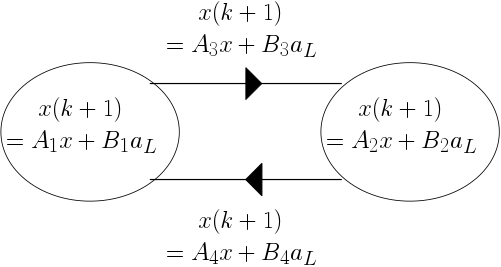
\includegraphics[scale=0.5]{fig/platton-dynamics.png}
\caption{Time discretized model of networked platoon}~\label{fig:model-platoon}
\end{figure}
%
%
\begin{table}
\caption{Matrices for discrete time slow switching model}~\label{matrices:slow}
{\scriptsize
$A_1=\mymatrix{0.2766  &  0.2855&   -0.0235&    0.2550&    0.2352&   -0.0429&    0.1245&    0.0956&   -0.0234\\
   -0.0917&   -0.0848&    0.0392&   -0.0517&    0.0134&    0.0023&    0.0003&    0.0385 &  -0.0166\\
   -0.0531&   -0.0485&    0.0404&    0.0434&    0.0807&   -0.0172&    0.0301&    0.0363&   -0.0097\\
    0.1406&    0.1632&    0.0002&    0.0313&    0.1166&   -0.0122&    0.1017&    0.1309&   -0.0431\\
   -0.0411&   -0.0589&   -0.0421&   -0.0512&   -0.1530&    0.0575&   -0.0476&   -0.0321&    0.0051\\
   -0.0393&   -0.0402&   -0.0111&   -0.0641&   -0.0754&    0.0467&    0.0497&    0.0760&   -0.0251\\
    0.0628&    0.0763&    0.0095&    0.0634&    0.0987&    0.0081&   -0.0788&    0.0489&   -0.0436\\
   -0.0088&   -0.0158&   -0.0081&   -0.0351&   -0.0452&   -0.0726&   -0.0621&   -0.2082&    0.0863\\
   -0.0246&   -0.0235&   -0.0078&   -0.0572&   -0.0547&   -0.0183&   -0.1049&   -0.1146&    0.0307}$
$A_2=\mymatrix{ 0.2398 &   0.2204&   -0.0715&   -0.0000&    0.0000&   -0.0000&   -0.0000&    0.0000&   -0.0000\\
   -0.1148&   -0.1083&    0.0352&   -0.0000&   -0.0000&    0.0000&   -0.0000&   -0.0000&    0.0000\\
   -0.0565&   -0.0567&    0.0176&   -0.0000&   -0.0000&   -0.0000&   -0.0000&   -0.0000&    0.0000\\
    0.0178&    0.5068 &  -0.0658&    0.2410&    0.3042&   -0.1113&   -0.0000&    0.0000&   -0.0000\\
   -0.1056&  -0.3026&    0.0327&   -0.1329&   -0.1627&    0.05657&   -0.0000&   -0.0000&    0.0000\\
   -0.1089&   -0.1100&   -0.0055&   -0.0675&   -0.0720&    0.0204&   -0.0000&   -0.0000&    0.0000\\
    0.2386&   -0.0802&    0.0965&    0.1118&    0.1544&    0.0604&    0.1197&    0.2679&   -0.1103\\
    0.0762&    0.3143&   -0.0998&   -0.0213&   -0.0283&   -0.0726&   -0.1404&   -0.2191&    0.0779\\
   -0.0043&    0.0212&   -0.0122&   -0.0468&   -0.0413&   -0.0171&   -0.0991&   -0.0990&    0.0251}$
 $B_1=\mymatrix{1.8593\\
    0.2855\\
    1.0848\\
    0.5394\\
    0.1632\\
    1.1437\\
    0.1950\\
    0.0763\\
    1.1596}$
$B_2=\mymatrix{1.7651\\
    0.2204\\
    1.1083\\
    2.1977\\
    0.5068\\
    1.4109\\
   -1.2748\\
   -0.0802\\
    1.0966}$
$B_3=\mymatrix{2.8411\\
    0.0019\\
    1.0006\\
    0.9508\\
    0.0007\\
    1.0009\\
    0.3775\\
    0.0003\\
    1.0009}$    
$B_4=\mymatrix{2.2276\\
    0.0001\\
    1.0001\\
    2.7152\\
   -0.0005\\
    1.0000\\
   -0.4469\\
    0.0001\\
    1.0000\\
}$
~~$A_3=A_4=\repmat{0}{9}{9}$.
}
\end{table}
%
\begin{table}
\caption{Matrices for discrete time fast switching model}~\label{matrices:fast}
{\scriptsize
$A_1=A_3=\mymatrix{ 0.8902 &   0.6370&   -0.1484&    0.0588&   -0.0050&    0.0001&    0.0157&   -0.0148&    0.0059\\
   -0.2340&    0.1889&   -0.1119&    0.1267&    0.0147&   -0.0039&    0.0363&   -0.0201&    0.0104\\
    0.1755&    0.7560&   -0.2251&   -0.0959&   -0.0989&    0.0181&   -0.0373&   -0.0273&    0.0018\\
    0.0462&    0.0643&    0.1514&    0.8509&    0.7076&   -0.1685&    0.0303&    0.0218&   -0.0038\\
    0.0934&    0.1271&    0.1151&   -0.3284&    0.2923&   -0.1466&    0.0660&    0.0517&   -0.0108\\
    0.1262&    0.6998&    0.0092&    0.1826&    0.7469&   -0.2119&   -0.0885&   -0.0830&    0.0189\\
    0.0116&    0.0170&    0.0026&    0.0241&    0.0282&    0.1719&    0.8532&    0.7238&   -0.1801\\
    0.0256&    0.0364&    0.0064&    0.0505&    0.0619&    0.1543&   -0.3320&    0.3231&   -0.1730\\
    0.1047&    0.6724&    0.0017&    0.1502&    0.6976&    0.0119&    0.2247&    0.7581&   -0.1875}$
$A_2=A_4=\mymatrix{0.8898 &   0.6325&   -0.1463&    0.0000&    0.0000&    0.0000&    0.0000&    0.0000&   -0.0000\\
   -0.2348&    0.1775&   -0.1094&    0.0000&    0.0000&    0.0000&    0.0000&    0.0000&   -0.0000\\
    0.1756&    0.7674&   -0.2136&    0.0000&    0.0000&    0.0000&    0.0000&    0.0000&   -0.0000\\
    0.0939&    0.3146&    0.1064&    0.9098&    0.6995&   -0.1686&    0.0000&    0.0000&   -0.0000\\
    0.1708&    0.6120&    0.0043&   -0.2012&    0.2985&   -0.1533&    0.0000&    0.0000&   -0.0000\\
    0.1687&    0.5757&    0.1151&    0.1829&    0.7569&   -0.1980&    0.0000&    0.0000&   -0.0000\\
   -0.0364&   -0.2331&    0.0460&    0.0254&    0.0312&    0.1721&    0.9004&    0.7304&   -0.1778\\
   -0.0529&   -0.4476&    0.1169&    0.0548&    0.0704&    0.1571&   -0.2263&    0.3541&   -0.1728\\
    0.1044&    0.6771&   -0.0016&    0.1418&    0.6953&    0.0121&    0.2199&    0.7571&   -0.1877}$    
$B_1=B_3=\mymatrix{0.3930\\
    0.6370\\
    0.8111\\
    0.0200\\
    0.0643\\
    0.6840\\
    0.0051\\
    0.0170\\
    0.6476\\
}$
$B_2=B_4=\mymatrix{0.3918\\
    0.6325\\
    0.8225\\
    0.0979\\
    0.3146\\
    0.2105\\
   -0.0727\\
   -0.2331\\
    0.6581}$
}
\end{table}
%

{\bf Time discretized models: } We could discretized the dynamics of
both models with large minimum switching time and integer switching
time.  The time discretized model has 2 locations and 4 edges, as
described in Figure~\ref{fig:model-platoon}.  The continuous state is
9-dimensional.  The matrices denoted in the figure are different for
the case of slow switching and fast switching and are given in
Tables~\ref{matrices:slow} and~\ref{matrices:fast}, respectively.


{\bf Linear invariance property: } The verification challenge proposed
in~\cite{makhlouf2014networked} is to find the minimum possible
reference distances $d_i^{ref}~\forall i\in\set{1,2,3}$, such that the
vehicles do not collide.  Any set of upper bounds on $-e_1$, $-e_2$,
and $-e_3$ are safe lower limits on the respective reference
distances.  We express the verification problem in terms of three
linear invariance properties, as follows.  For each ${T_i:~1\leq i\leq
3}$, where
%
$ T_1=\mymatrix{-1 & \repmat{0}{1}{8}},~
T_2=\mymatrix{\repmat{0}{1}{3} & -1 &\repmat{0}{5}{3}}$ and
 ${T_3=\mymatrix{\repmat{0}{1}{6}& -1 &\repmat{0}{2}{3}}},
$
%
find an upper bound on each $d_i:~i\in\set{1,2,3}$ such that
$\lt(T_i,d_i\rt)$ is a linear invariance property of the system.

\tbf{Experiment settings.}  We chose the primary template
as the collection of the (complex) eigenvectors of linear matrices of
the affine maps in the the two locations and their binary products,
the axis aligned box template and the templates used for
overapproximating the input sets. For the SpaceEx tool, we
experimented with two templates, octagon and hundred uniformly sampled
support vectors.

\tbf{Results.}  For the large minimum dwell time of $20s$, the
discrete time SpaceEx implementation and also a method based on using
real zonotopes~\cite{makhlouf2014networked} could verify slightly
smaller bounds compared to our approach.  But for the small minimum
dwell time ($1s$) model, SpaceEx could not even find a finite set of
bounds, whereas our approach could verify a finite set of bounds.  The
reason is that the fast system model is more stable compared to the
slow switching.  Possibly because complex zonotope captures
contraction along complex eigenvectors, we could find a finite
invariant for even the less stable fast switching model.  These
results are reported in the Tables~\ref{tab:largedwell-platoon}
and~\ref{tab:largedwell-platoon1}.
%

\begin{table}
\begin{tabular}{|l|c|c|c|c|c|}
\hline
\multicolumn{2}{|c|}{\multirow{4}{*}{Method}} & \multicolumn{4}{|c|}{\multirow{2}{*}{Slow switching}}\\
\multicolumn{2}{|c|}{} & \multicolumn{4}{|c|}{}\\
\cline{3-6}
\multicolumn{2}{|c|}{} & \multirow{2}{*}{$-e_1\leq$} & \multirow{2}{*}{$-e_2\leq$} & \multirow{2}{*}{$-e_3\leq$} & Comp.\\
\multicolumn{2}{|c|}{} & & & & time (s)\\
\hline
\multirow{4}{*}{SpaceEx} & octagon & \multirow{2}{*}{28} &
\multirow{2}{*}{27} & \multirow{2}{*}{10}& \multirow{2}{*}{$>180s$}\\
& template & & & &\\
\cline{2-6}
& 100 support & \multirow{2}{*}{28} & \multirow{2}{*}{25} &
\multirow{2}{*}{13} & \multirow{2}{*}{1.3}\\
& vectors & & & &\\
\hline
\multicolumn{2}{|c|}{\multirow{2}{*}{Real zonotope~\cite{makhlouf2014networked}}} &
\multirow{2}{*}{25} & \multirow{2}{*}{25} & \multirow{2}{*}{10} & \multirow{2}{*}{n/a}\\
\multicolumn{2}{|c|}{} & & & &\\
\hline
\multicolumn{2}{|c|}{\multirow{2}{*}{Augmented complex zonotope}} &
\multirow{2}{*}{28} & \multirow{2}{*}{26} &
\multirow{2}{*}{12} & \multirow{2}{*}{12}\\
\multicolumn{2}{|c|}{} & & & & \\
\hline
\end{tabular}
\caption{Experimental results: Slow switching networked platoon}~\label{tab:largedwell-platoon}

%% %
%% \end{table}
%% %
%% \begin{table}
{\vspace{2em}
\begin{tabular}{|l|c|c|c|c|c|}
\hline
\multicolumn{2}{|c|}{\multirow{4}{*}{Method}} & \multicolumn{4}{|c|}{\multirow{2}{*}{Fast switching}}\\
\multicolumn{2}{|c|}{} & \multicolumn{4}{|c|}{}\\
\cline{3-6}
\multicolumn{2}{|c|}{} & \multirow{2}{*}{$-e_1\leq$} & \multirow{2}{*}{$-e_2\leq$} & \multirow{2}{*}{$-e_3\leq$} & Comp.\\
\multicolumn{2}{|c|}{} & & & & time (s)\\
\hline
\multirow{4}{*}{SpaceEx} & octagon & \multirow{2}{*}{$>1000$} &
\multirow{2}{*}{$>1000$} & \multirow{2}{*}{$>1000$} &
\multirow{2}{*}{$>180s$}\\
& template & & & &\\
\cline{2-6}
& 100 support & \multirow{2}{*}{$>1000$} & \multirow{2}{*}{$>1000$} &
\multirow{2}{*}{$>1000$} & \multirow{2}{*}{$>180s$}\\
& vectors & & & & \\
\hline
\multicolumn{2}{|c|}{\multirow{2}{*}{Augmented complex zonotope}} &
\multirow{2}{*}{46} & \multirow{2}{*}{54} &
\multirow{2}{*}{57} & \multirow{2}{*}{12.6}\\
\multicolumn{2}{|c|}{} & & & & \\
\hline
\end{tabular}
%
\caption{Experimental results: Fast switching networked Platoon}~\label{tab:largedwell-platoon1}
}
\end{table}



\subsection{Perturbed double integrator}
Our second example is a perturbed double integrator system given
in~\cite{rakovic2004computation}.  The closed loop system with a
feedback control is piecewise affine, having four different affine
dynamics in four different regions of space, as
%
\begin{align*}~\label{eqn:pwa-regions}
& \trj{x}{t+1}=M_i\trj{x}{t}+w.~~~
 i=\left\{\begin{array}{l}
1,~\text{if}~x_1\geq 0~\text{and}~x_2\geq 0\\
2,~\text{if}~x_1\leq 0~\text{and}~x_2\leq 0\\
3,~\text{if}~x_1\leq 0~\text{and}~x_2\geq 0\\
4,~\text{if}~x_1\geq 0~\text{and}~x_2\leq 0\\
\end{array} \rt.,\\
&~M_1=M_2=\lt[\begin{matrix}
0.4103  &  0.0653\\
  -0.2949  &  0.5327
\end{matrix}\rt],~M_3=M_4=\lt[\begin{matrix}
0.4103  &  -0.0653\\
  0.2949  &  0.5327
\end{matrix}\rt].
\end{align*}

The additive disturbance input $w$ is bounded as $\|w\|_{\infty}\leq
0.2$.  

We perform two different experiments on this system.  In the first
experiment, we try to verify the smallest possible magnitude of bounds
on the two coordinates, denoted $x_1$ and $x_2$. We compare these
bounds with that found by the SpaceEx tool.  In the second experiment,
we try to quickly compute a large invariant for the system under the
safety constraints given in~\cite{rakovic2004computation}.  The given
safety constraints are $\|x\|_{\infty}\leq 5$.  In the latter case, we
maximize the sum of the scaling factors and differences of the upper
and lower interval bounds of the augmented complex zonotopic
invaraint.  Furthermore, we decompose the given safety constraints as
the intersection of four different sets of safety constraints.  For
each set of safety constraints, we compute a large augmented complex
zonotopic invariant.  Then the desired invariant is the intersection
of four augmented complex zonotopic invariants.  Although we may not
find the largest possible (maximal) invariant by this approach, still
the optimizer will try to maximize the size of the invariant.  We draw
comparison in terms of the computation time with the reported result
for the MPT tool~\cite{rakovic2004computation}.

In our formalism, we model the system with $4$ locations and $12$
edges connecting all the locations.  Appropriate staying conditions
are specified in each location, reflecting the division of the state
space into different regions where the dynamics is affine. The initial
set is the origin. The same model is specified in SpaceEx.

\tbf{Size of model}: 2 dimensions, 4 locations and 12 edges.

\tbf{Experiment settings}.  For the primary template, we collected the
(complex) eigenvectors of all linear matrices of the affine maps and
their binary products. For the SpaceEx tool, we experimented with two
different templates, the octagon template and a template with 100
uniformly sampled support vectors.

\tbf{Results.}  In the first experiment, we verified sligtly smaller bounds
for $x_1$ than that of SpaceEx, while the bounds verified for $x_2$
were equal for both methods.  In our second experiment on this
example, the computation time for finding a large invariant by our
method is significantly smaller than that of the reported result for
the MPT tool.  The results are summarized in the
Tables~\ref{tab:smallinv-pdi} and~\ref{tab:largeinv-pdi}.

\begin{table}
\center
\begin{tabular}{|l|c|c|c|c|}
\hline
\multicolumn{2}{|c|}{\multirow{2}{*}{Method}} &
\multirow{2}{*}{$\lt|x_1\rt|\leq$} & \multirow{2}{*}{$\lt|x_2\rt|\leq$} & Comp.\\
\multicolumn{2}{|c|}{} & & & time (s) \\
\hline
\multirow{4}{*}{SpaceEx} & octagon & \multirow{2}{*}{0.38} &
\multirow{2}{*}{0.43} & \multirow{2}{*}{1.7}\\
& template & & &\\
\cline{2-5}
& 100 support & \multirow{2}{*}{0.38} & \multirow{2}{*}{0.43} & \multirow{2}{*}{23.6}\\
& vectors & & &\\
\hline
\multicolumn{2}{|c|}{\multirow{2}{*}{ACZ invariant}} &
\multirow{2}{*}{0.37} & \multirow{2}{*}{0.43} & 
\multirow{2}{*}{5.1}\\
\multicolumn{2}{|c|}{} & & &\\
\hline
\end{tabular}
\caption{Small invariant computation: Perturbed double
  integrator}
~\label{tab:smallinv-pdi}
\end{table}
%
\begin{table}
\center
\begin{tabular}{|c|c|}
\hline
\multirow{2}{*}{Method} & Comp.\\
& time (s)\\
\hline
\multirow{2}{*}{MPT tool~\cite{rakovic2004computation}} & \multirow{2}{*}{107}\\
& \\
\hline
\multirow{2}{*}{ACZ} & \multirow{2}{*}{12}\\
& \\
\hline
\end{tabular}
\caption{Large invariant computation: Perturbed double integrator}
~\label{tab:largeinv-pdi}
\end{table}
%% \tbf{Remark.}  The overapproximation quality of SpaceEx reduces when
%% there are large number of edges, because then in each step, a union of
%% many different polytopes has to be overapproximated using support
%% vectors.  In contrast, our approach uses optimization to learn an
%% appropriate invariant, avoiding the union operations.  Possibly
%% because of this reason, we verified smaller bounds than SpaceEx on
%% this example.



\section{TODO}

%
\chapter{Stability Verification of Nearly Periodic Linear Impulsive Systems} ~\label{ch:lis} 

    Since computers work with digital signals and the physical system
    they control operates in the analog world, sampling is required.
    Various parameters related to sampling of the system can be
    subject to uncertainty like the sampling period, delay, digital
    output of the controller, output feedback from the system, etc.
    These uncertainties can lead to instability of the system.
    Henceforth, we are faced with the challenge of verifying system
    stability in the presence of these uncertainties.  We address this
    issue by considering the problem of verifying stability of
    nearly-periodic impulsive systems, which can be used to model
    sampled-data systems \cite{naghshtabrizi2007delay} and networked
    control systems \cite{2008-naghshtabrizi-exponential}.  This
    problem has been tackled using control approaches, which mainly
    involve deriving stability conditions in terms of Lyapunov
    functions and checking these conditions using optimization (Linear
    Matrix Inequalities (LMI) or Sum of Squares (SOS)). In this work,
    we use a stability condition based on set contractiveness proposed
    in
    \cite{athanasopoulos2014alternative,2014-fiacchini-set,AlKhatib2015}
    and propose a new method for checking it using computational
    techniques, inspired by hybrid systems verification
    techniques. Globally exponential stability (GES) of
    nearly-periodic linear impulsive systems can be proved by showing
    the contractiveness of a compact and convex set containing the
    origin in its interior, also called as a $C$-set
    \cite{Lazar2013,athanasopoulos2014alternative,2014-fiacchini-set,AlKhatib2015}.
    The uncertainty in impulse times for which stability can be proved
    depends on the choice of the contractive $C$-set.  A
    nearly-periodic linear impulsive system is stable only if all of
    its reachability operators, which compute the state reached after
    an impulse, are stable.  This motivates us to use complex
    zonotopes since we can find good candidate complex zonotope for
    contractive sets using the eigenvectors of the reachability
    operators.  For proving stability condition, we consider complex
    zonotopes whose generator sets are chosen among the eigenvectors
    of reachability operators of the nearly-periodic linear impulsive
    system.  We then derive a condition for the contractiveness of a
    complex zonotope that can be verified by convex optimization.
    Concerning experimental results, our approach is either
    competitive or better compared to the existing approaches, in
    terms of the largeness of uncertainty of sampling periods for
    which stability could be proved.

    The chapter is organized into five main sections.  We discuss the
    related work in Section~\ref{lis-rel}.  In
    Section~\ref{sec:dynamics}, we describe the dynamics of a
    nearly-periodic linear impulsive system.  In
    Section~\ref{sec:ges}, we explain global exponential stability,
    the verification problem and its relation to finding a contractive
    $C$-set of the system.  In Section~\ref{sec:alg}, we explain our
    algorithm for stability verification based on complex zonotopes.
    The experiments on two benchmark examples are discussed in Section~\ref{sec:experiments}



\section{Related work}~\label{lis-rel}
A major approach to stability analysis of aperiodic sampling control uses time-delay 
systems, and stability can be proved using Lyapunov Krakovskii functional 
\cite{Mikheev1988,Teel1998,2010-liu-stability,Mazenc2013}, 
or time-dependent Lyapunov functional \cite{2010-fridman-refined}. Using a continuous-time model,  
discrete-time Lyapunov functions is proposed for stability condition \cite{2012-seuret-novel}, 
which can be checked using Sum of Squares (SOS) \cite{2013-seuret-stability}. Robust stability with respect to 
time-varying input delay can also be handled by input/output approach 
\cite{Mirkin2007,DBLP:journals/automatica/Fujioka09,DBLP:conf/amcc/KaoW14,Omran2013,Omran2014}.
Another important approach is based on the hybrid systems modeling framework, in particular time-varying impulsive systems 
\cite{Hu2003,nevsic2004framework,Goebel2009,Cai2008,BauLoo_NECSYS12a} and employs Lyapunov-based 
methods in various forms including discontinuous time-independent \cite{2008-naghshtabrizi-exponential} 
or time-dependent Lyapunov functions \cite{2010-fridman-refined}. Another popular 
approach involves using convex embedding \cite{HetelDaafouz2006,Fujioka2009,HetelKruszewski2011,2013hetel,Omran2014}. 
In this approach, stability tests can be formulated as parametric Linear Matrix Inequalities (LMIs) \cite{HetelDaafouz2006}, 
or as set contractiveness (such as, polytopic set contractiveness is equivalent to polyhedral Lyapunov 
functions) \cite{2014-fiacchini-set,2013-briat-convex,Lazar2013,athanasopoulos2014alternative,AlKhatib2015}. 
In this work, we focus on exponential stability and are inspired by
set theory conditions
\cite{2014-fiacchini-set,athanasopoulos2014alternative,AlKhatib2015} to derive a stability condition which is more conservative 
but can be efficiently verified. The novelty of our work lies in the use of complex zonotopes to efficiently 
find contractive sets. Computationally speaking, our approach is close in spirit to abstract interpretation
and hybrid systems analysis. Indeed the way we find contractive sets using such zonotopes is similar 
to the way invariant sets are computed using some zonotope
\cite{Girard05reachabilityof,Althoff2011,DBLP:conf/sas/GoubaultPV12} and
template-polyhedral abstract domains \cite{Sriram2008,jeannet2009apron}.



\section{Dynamics}~\label{sec:dynamics}
In a discrete time affine hybrid system, the state of the system is
specified by a discrete valued variable, called location, and a
continuous variable whose valuation is in the real Euclidean space of
a finite dimenstion.  The state of the system in each location has to
stay within a polyhedral set, called the staying condition.  The state
of the system can change by two kinds of transitions, {\it continuous
  transition} and {\it discrete transiton}.  In a continuous
transition, the discrete state of the system remains constant while
the continuous state changes by an affine transformation.  The affine
transformation has possible additive disturbance input, which is
bounded.  The parameters of the affine transformation of a continuous
transition depend on the location in which the transition takes place.
In a discrete transition, there is a change in the discrete variable
accompanied by an affine transformation of the continuous variable.
The transition is has precondition specified by a linear constraint,
called a guard, while the post-condition is the staying condition in
the location reached after transition.  A set of edges specifies
the possible discrete transitions, vis a vis, the locations between
which a discrete transition takes place, the parameters of the affine
transformation and the guard.   

{\it Sub-parallelotopic guards and staying conditions}: In this paper,
we consider hybrid systems where the guards and staying conditions can
be specified by a sub-parallelotope with a common template.  We note
that the class of sub-parallelotopic constraints are quite general and
can be used in the specification of many practical affine hybrid
systems.  

{\bf Model.}  We specify the discrete time affine hybrid system
by a tuple 
 %
\[
\system = \lt(\locations,\qtemp,\stay,\linmap,\inputset,\edgeset,\Psi\rt).
\]
%
The finite set of locations is $\locations$.  The sub-parallelotopic
template for specifying the guards and staying conditions is
$\qtemp\in\mat{k}{n}{\reals}$.  The staying set in a location
$\loc\in\locations$ is a sub-parallelotope
$\ptope{\qtemp}{\lsys{\stay_\loc}}{\usys{\stay_\loc}}$, whose pair of
lower and upper interval bounds is
$\stay_\loc=\lt(\lsys{\stay_\loc},\usys{\stay_\loc}\rt)$ .  The
parameters affine transformation in a location $\loc\in\locations$
consist of a linear transformation, specified by a matrix
$\linmap_\loc\in\mat{n}{n}{\reals}$, and a bounded additive
disturbance input set $\inputset_\loc\subset\reals^n$.  The set of
edges is $E$.  An edge $\edge\in\edgeset$ is specified by a tuple
%
\[
\edge=\lt(\edge_1,\edge_2,\usys{\edge},\lsys{\edge},\linmap_\edge,\inputset_\edge\rt).
\]
%
The before and after locations of a discrete transition along an edge
$\edge$ are $\edge_1,\edge_2$.  The guard on the transition along the
edge $\edge$ is the sub-parallelotope
$\ptope{\qtemp}{\lsys{\edge}}{\usys{\edge}}$, whose pair of
lower and upper interval bounds is
$\lt({\lsys{\edge}},{\usys{\edge}}\rt)$.
The parameters of the affine transformation for the discrete
transition along the edge $\edge$ consists of a linear map specified
by the matrix $\linmap_\edge\in\mat{n}{n}{\reals}$ and a bounded
additive disturbance input set $\inputset_\edge\subset\reals^n$.  The
set of initial states of the system is $\Psi\subseteq\locations\times\reals^n$.

{\bf Dynamics.}  A state of the hybrid system is a pair $(x,\loc)$,
where $x\in\reals^n$, called the {\it continuous state}, and
$\loc\in\locations$, called the {\it discrete state}.  A {\it
  trajectory} specifies the evolution of the state of the system as a
function of discrete time instants.  A trajectory is a function
$\maphtrj:\integers_{\geq 0}\ra\reals^n\times\locations$, such that
$\forall t\in\integers_{\geq 0}$, one of the following conditions is
true.
%
\begin{enumerate}
\item todo
\item todo
\end{enumerate}
%































{\color{red} TODO.}

\section{Globally exponential stability and set contraction}~\label{sec:ges}
A nearly periodic linear impulsive system is globally exponentially
stable (GES) if any point in the state space reaches arbitrarily close
to the origin at an exponential rate.  This property is mathematically
stated as follows.
%
\begin{defn}\label{defn:exp-stable}[Global exponential stability (GES)] The
system $\system$ is globally exponentially stable
(GES) if there exists $\lambda\in[0,1)$ and $c>0$ such that for all $\initstate
\in\mb{R}^n$ and $k\in\mb{Z}_+$,
$||\tbf{x}_k||\leq c\lambda^k||\tbf{x}_0||$.
\end{defn}
%
The following is the stability verification problem.
%
\begin{problem}
Given a sampling period interval $\Delta=[\lsb,\usb]$, verify
that the system $H$ is globally exponentially stable.
\end{problem}
%
The GES of a system is related to the reachable sets of the
system. Indeed if all bounded sets containing the origin eventually
contract to arbitrarily small sets around the origin, then every point
eventually reaches close to the origin and the system is thus
GES. Instead of verifying the contraction of all bounded sets
containing the origin, we can verify the contraction of any compact
and convex set containing the origin, because it can be scaled to
include any bounded set. We
call such sets as $C$-sets.

The contractiveness of a set is defined as follows.
%
\begin{definition}[\cite{2014-fiacchini-set}]
Given $\lambda\in[0,1]$, a set $C$-set $\Psi\subset\reals^n$ is
$\lambda$-contractive for the system $\system$ iff
\[\forall x\in\Psi,~\forall t\in\Delta,~H_tx\in\lambda\Psi.\]
\end{definition}
%
\begin{remark} It has been shown previously
in~(\cite{2014-fiacchini-set,athanasopoulos2014alternative,AlKhatib2015})
that globally exponentially stablility of a nearly-periodic linear
impulsive system is equivalent to the existence of a
$\lambda$-contractive $C$-set for a $\lambda\in[0,1)$.  So, we can
  find a $\lambda$-contractive $C$-set for $\lambda<1$ to prove  global
  exponential stability.
\end{remark}
%
  A stability verification algorithm was proposed
  in~\cite{2014-fiacchini-set} that definitely computes a contractive
  $C$-set for a globally exponentially stable system.  But the
  algorithm involves iterative intersections.  But during iterative
  intersections, the complexity of representing the set can grow
  uncontrollably.  So, the
  algorithm~\cite{2014-fiacchini-set} can be costly, especially in
  higher dimensions.  Alternatively, we propose a stability
  verification algorithm using complex zonotope and convex
  optimization, where the size of the template is fixed apriori.
  Although the existence of a contractive complex zonotope is only a
  sufficient condition for global exponential stability, we demostrate
  the efficiency of our procedure by experiments on some benchmark
  examples.  Our algorithm, described in the next section, uses some
  properties of contraction of sets, which we shall discuss now.

Since the state change of the system can be identified by the
transformation by a reachability operator, we define contraction by
a matrix as follows.  From here on, we denote $J$ as an
$n\times n$ real matrix.
%
\begin{defn} The amount of contraction of a set
  $\Psi\subset\mathbb{R}^n$ upon transformation by the matrix $J$,
  denoted as $\chi(\Psi,J)$, is $$\chi(\Psi,J) =
  \inf\{a\in\mathbb{R}_{\geq 0} : J(\Psi)\subseteq a
  \Psi\}.$$ \end{defn}
% \begin{defn} The amount of contraction of a set $\Psi\subset\mathbb{R}^n$
% after $k$ steps for some $k\in\mathbb{Z}^+$, denoted by  $\chi_k(\Psi)$, is
% $$\chi_k(\Psi)=\inf\{a\in\mathbb{R}_{\geq 0} : R^k(\Psi)\subseteq a\Psi\}.$$  
% %We shall denote the contraction of $\Psi$ after $k$ steps as $\chi_k(\Psi)$.
% \end{defn}
The amount of contraction being greater than one would indicate that
the set is actually \emph{expanding}, which will also be referred
mathematically as ``contraction'' parameter, in a general sense.
%
%
For any $\rho:0\leq \rho\leq \epsilon$, we want to derive a bound on the
contraction of the operator $H_{t+\rho}$ as a function of $H_t$ and
$\epsilon$.  Using Taylor expansion of an order $r$, we
can write
\begin{align*}
&
  H_{t+\rho}=e^{(A_c\rho)}H_t=P_r(\rho)H_t+E_r(\delta)H_t~~\text{where}\\
&  P_r(\rho)=\sum_{i=0}^r\frac{A_c^i\rho^i}{i!},~~~~~~
 E_r(\delta)=\frac{A_c^{r+1}\delta^{r+1}}{(r+1)!}:~~\delta\in[0,\epsilon].~\numberthis\label{eqn:taylor}
\end{align*}
%
To use the above expansion for deriving the bound on contraction, we
shall describe some of its properties.  The following
lemma states that the contraction upon transformation
by the product of any two matrices is bounded by the product of the
contractions by individual matrices.  Also, the contraction
upon transformation by the sum of two matrices is bounded by the sum
of the contractions by the individual matrices.
%
\begin{lem}\label{lem:composition}
Let us consider $J_1,J_2\in\mat{n}{n}{\reals^n}$ and
  $\Psi\subset\reals^n$.  Then the all of the following is true.
\begin{enumerate}
\item $\chi(\Psi,J_1+J_2)\leq\chi(\Psi,J_1)+\chi(\Psi,J_2)$.
\item $\chi(\Psi,J_1J_2)\leq\chi(\Psi,J_1)\chi(\Psi,J_2)$.
\end{enumerate}
\end{lem}
%
\begin{proof}
  For proving the first part, we derive the following.
  %
  \begin{align*}
&  \text{Since}\hspace{1em}   J_1\Psi\subseteq
    \chi(\Psi,J_1)\Psi~\text{ and }
    J_2\Psi\subseteq \chi(\Psi,J_2),~\text{we get}\\
&  (J_1+J_2)\Psi\subseteq
  \chi(\Psi,J_1)\Psi \oplus \chi(\Psi,J_2)\Psi=
  (\chi(\Psi,J_1) + \chi(\Psi,J_2))\Psi.
  \end{align*}
  %
For proving the second part, we derive the following.
\begin{align*}
  &  J_1J_2\Psi=J_1(J_2\Psi)\subseteq J_1(\chi(\Psi,J_2)\Psi)\\
 &=\chi(\Psi,J_2)\lt(J_1\Psi\rt)\subseteq
  \chi(\Psi,J_1)\chi(\Psi,J_2)\Psi.\hspace{3em}\qedhere
\end{align*}
%
\end{proof}
%
If a matrix is embedded inside the convex hull of a set of matrices,
then we get the following bound on contraction by the matrix.
%
\begin{lemma}~\label{lem:conv-bound}
Let us consider that $J\in\convexhull{\set{A_1,...,A_r}}$ and
$\Psi\subset\reals^n$.  Then
%
\begin{align*}
& \contraction{J}{\Psi}\leq\max_{i=1}^r\contraction{A_i}{\Psi}.
\end{align*}
%
\end{lemma}
%
\begin{proof}
As $J\in\convexhull{\set{A_1,...,A_r}}$, there exists
$\alpha_1,...,\alpha_r\in\reals_{\geq 0}$ such that
$\sum_{i=1}^r\alpha_i=1$ and $J=\sum_{i=1}^r\alpha_iA_i$.  Then by
using Lemma~\ref{lem:composition}, we get
%
\begin{align*}
  & \contraction{J}{\Psi}\leq\sum_{i=1}^r\alpha_i\contraction{A_i}{\Psi}\\
  & \leq \lt(\sum_{i=1}^r\alpha_i\rt)\max_{i=1}^r\contraction{A_i}{\Psi}=\max_{i=1}^r\contraction{A_i}{\Psi}.\hspace{3em}\qedhere
\end{align*}
%
\end{proof}
%
If we want to bound the contraction of a polynomial with matrix
co-coefficients, where the variable has a bound, then the following
lemma is useful.  The set of all possible values of
the polynomial can be embedded inside a convex hull of a finite set of
matrices, as described below.
%
\begin{lem}~\label{lem:convex}~\cite{2013hetel}
Let us consider $\set{A_0,A_1,...,A_r}\subseteq\mat{n}{n}\reals$ where
%
\[
\forall j\in\{0,...,r\},~ U_j(\rho)=\sum_{i=0}^jA_i\rho^i.
\]
%
If
$0\leq\rho\leq \epsilon$, then $U_r(\rho)\in
\convexhull{U_0(\epsilon),U_1(\epsilon),...,U_r(\epsilon)}$.
\end{lem}
\begin{proof}
This has been proved in~\cite{2013hetel}.
\end{proof}

Using the above results, we derive the following bound on contraction
by the operator $H_{t+\rho}$, when $\rho\in[0,\epsilon]$.
%
\begin{lemma}\label{lem:conv}
Let us consider $\Psi\subset\reals^n$ and $\rho\in[0,\epsilon]$.  If
$0\leq \rho\leq \epsilon$, then
%
\begin{align*}
& \contraction{H_{t+\rho}}{\Psi}\leq\max_{i=1}^r\contraction{P_r(\epsilon)H_t}{\Psi}+\contraction{\frac{A_c^{r+1}}{(r+1)!}H_t}{\Psi}\epsilon^{r+1}.
\end{align*}
%
\end{lemma}
%
\begin{proof}
Using Equation~\ref{eqn:taylor}, there exists
$\delta\in[0,\epsilon]$ such that,
%
\begin{align*}
&
  \contraction{H_{t+\rho}}{\Psi}=\contraction{P_r(\rho)+E_r(\delta)}{\Psi}\\
& \%\%~~\text{by Lemma~\ref{lem:composition}}\\
&
  \leq\contraction{P_r(\rho)H_t}{\Psi}+\contraction{\frac{A_c^{r+1}}{(r+1)!}H_t}{\Psi}\delta^{r+1}\\
  & \%\%~~\text{by Lemmas~\ref{lem:conv-bound} and~\ref{lem:convex}}\\
&
  \leq\max_{i=1}^r\contraction{P_r(\epsilon)H_t}{\Psi}+\contraction{\frac{A_c^{r+1}}{(r+1)!}H_t}{\Psi}\delta^{r+1}\\
& \leq\max_{i=1}^r\contraction{P_r(\epsilon)H_t}{\Psi}+\contraction{\frac{A_c^{r+1}}{(r+1)!}H_t}{\Psi}\epsilon^{r+1}.\hspace{3em}\qedhere
\end{align*}
%
\end{proof}
%





\section{Stability verification using complex zonotope}~\label{sec:alg}
{\color{red} TODO}.

\section{Experiments}~\label{sec:experiments}
\subsection{Robot with a saturated controller}
Our first example is a veriication problem for the model of a
self-balancing two wheeled robot called
NXTway-GS1\footnote{\url{http://www.mathworks.com/matlabcentral/fileexchange/19147-nxtway-gs-self-balancing-two-wheeled-robot-controller-design}}
by Yorihisa Yamamoto, which was presented in the ARCH
workshop~\cite{heinz2014benchmark}. We consider the linearized sampled
data (discrete time) networked control system model from the paper.
The state of the plant is represented by a 6-dimensional vector
$x_p=(\dot{\theta},\theta,\dot{\psi},\psi,\dot{\phi},\phi)^T$, where
$\theta$ is the average angle of the left and right wheel, $\psi$ is
the body pitch angle, $\phi$ is the body yaw angle, and the rest
coordinates are their respective angular velocities.  The output of
the plant is represented by a 3-dimensional vector
$\lt(\dot{\psi}_{\operatorname*{out}},\theta_{m_1},\theta_{m_r}\rt)^T$
such that $y_p=C_px_p$.  The input to the plant is a two dimensional
vector $u_p$.  The dynamics of the plant is given by the differential
equation $\dot{x}_p=A_px_p+B_pu_p$.  In the sampled data system, the
state of the plant is sampled every 4s.

The controller state is represented by a 6-dimensional vector $x_c$,
and the input to the controller is denoted
$u_c=\lt({u^\pr}_c,u^\dpr_c\rt)$.  The controller inputs
${{u^\pr}_c}$ and $u^\dpr_c$ are both 2-dimensional inputs.  The input
$u^\dpr$ is an uncertain input which is in the range $[-100,100]$.  The
controller dynamics is given by the equations
%
\begin{align*}
  & \dot{\tau}=1,~~\tau(4^+)=0\\
  & {u^\pr}_c(\tau)=\hat{u}_c(0)~\text{if}~\tau\in[0,4)\\
  & {u^\pr}_c(4)=y_p(\tau)\\
  & \dot{x_c}(\tau)={A}_cx_c(\tau)+{B}_cu_c(\tau)\\
  & y_c(\tau)=C_cx_c(\tau)+D_cu_c(\tau).
\end{align*}
%
The controller has a 2-dimensional output $y_c$ which is processed to
provide input to the plant.  The processor has a saturation limit on
the output received from the controller.  The saturated controller
output is given by the equation
%
\begin{align*}
u_p=D_p\lt(\join{\lt(\meet{y_c}{\mymatrix{v\\v}}\rt)}{\mymatrix{-v\\-v}}\rt).~\numberthis\label{eqn:sat1}
\end{align*}
%
where $v=100$ is a saturation limit.  The sampled data dynamics with
saturation can be modeled by an affine discrete time hybrid system,
where the switching is controlled by relevant guards on $u_p$.
However, if we consider the continuous state of the affine hybrid
system as $\lt(x_p,x_c,u_p\rt)^T$, we observed that some of the
directions are unbounded.  Therefore, we decoupled some unbounded
directions of the dynamics from the bounded directions by making
appropriate linear transformation of the coordinates.  The linear
transformation is composed by two transformations, one of which
involved Jordan decomposition in Matlab.

\begin{table}
{\scriptsize
\begin{align*}
& F_1  = \lt[\begin{matrix}
3.6929   &      0  &  0.7302  &  7.9715 &  14.5019 &   -0.0072 &
0.0720 &   -2.7354\\
    3.6929   &      0  &  0.7302  &  7.9715 &  14.5019 &  -0.0072  &  0.0720  & -2.7354\\
    0.9562    &     0  &  0.0019 &  -0.0021 &  -0.0022 &   -0.0000 &  -0.0001 &  -0.0002\\
         0 &   0.6910    &     0    &     0  &       0     &    0   &      0    &     0\\
    0.8833     &    0  & -0.1154 &  -1.2943 &  -2.3520  &  0.0012 &  -0.0118  &  0.4427\\
   -0.4712    &     0 &  -0.0812 &    0.1151  & -1.4845  &  0.0007 &  -0.0071  &  0.2819\\
   -0.1560     &    0 &  -0.0459 &  -0.3173  &  0.3650  &  0.0003  & -0.0023  &  0.1162\\
   -0.7719   &      0 &  -0.1248  & -1.4264 &  -2.5901  &  0.9973 &  -0.0131  &  0.4869\\
   -0.7544  &       0  & -0.1243 &  -1.4204 &  -2.5792  &  0.0013 &   0.9825 &   0.4796\\
   -0.1905   &      0  & -0.0148  & -0.2081 &  -0.3751  &  0.0002  &  0.0033  &  1.0651
\end{matrix}\rt]\\
& F_2 = \lt[\begin{matrix}
0.2543  &  0.2543\\
    0.2543  &  0.2543\\
   -0.0001 &  -0.0001\\
         0 &        0\\
   -0.0413 &  -0.0413\\
    0.0219  &  0.0219\\
    0.0102 &   0.0102\\
    0.0431 &   0.0431\\
    0.0428 &   0.0428\\
    0.0065 &   0.0065\\
\end{matrix}\rt],
~F_3 = 10^{-2}\times\lt[\begin{matrix}
 0.0000    &     0  & -0.0330 &   2.0218\\
    0   &      0  & -0.0330 &  -2.0218\\
    0  &       0 &   -0  &  0\\
   -0  &       0  &  0 &   0.0109\\
   -0.0118 &        0  &  0.0172  &  0 \\
    0.0436  &       0 &   0.0003 &  0 \\
   -0.0478   &      0  &  0.0034 &   0 \\
  -13.3924 &        0 &   0.0062 &   0 \\
    0.0909     &    0  &  0.0061 &  0\\
   -0.0798  &       0 &   0.0017  &  0\\
\end{matrix}\rt]
\end{align*}}
\caption{Matrices of the transformed system dynamics}~\label{tab:matrices-nxt}
\end{table}


After decomposition, the bounded dynamics with saturation could be
modeled in a 10-dimensional state space, which is described below.
%
\begin{align*}
\mymatrix{x(t+1)\\y(t+1)}=F_1\trj{x}{t}+F_2sat\lt(\trj{y}{t}\rt)+F_3\trj{u}{t},
\end{align*}
where $\trj{x}{t}\in\realset^8$ is the transformed state of the
composite system of plant and controller, $\trj{y}{t}\in\realset^2$ is
the input sent by the controller, $\trj{u}{t}\in\lt[-100,100\rt]^4$ is
the bounded additive disturbance input and $\operatorname*{sat}$ is
the saturation function which limits the controller input received by
the plant.  The body pitch angle is the first co-ordinate, i.e.,
$\psi=x_1$.  The matrices $F_1$, $F_2$ and $F_3$ are given in
Table~\ref{tab:matrices-nxt}.  The matrices for the original
(untransformed system) are given in the appendix.  The saturation
function is defined as follows.  The saturation function is given as
follows.
%
\begin{align*}
& \text{If
  saturated}~~\operatorname*{sat}\lt(y_i\rt) = max\lt(-\delta
 d_p,min\lt(y_i,\delta d_p\rt)\rt),~\forall i\in\{1,2\},\\
&\text{If unsaturated}~~ sat\lt(y_i\rt)=y_i~\forall i\in\{1,2\}.
\end{align*}
%
where $\delta=100$ and $d_p=0.0807$.  
%
{\color{red} TODO Input figure here}.

{\bf Model complexity:} The 2-dimensional input $y$ on which the
positive and negative saturation is defined can thus be divided into 9
different regions, where the system exhibits different dynamics.  We
model each of the discrete time dynamics by a self edge on a common location.
Therefore, the saturated model consists of a single location with 9
self-edges having appropriate linear guards and transition matrices.
On the other hand, the unsaturated model is a linear system having
uncertain input, which is therefore modeled by only one location.

\emph{Size of saturated model}: 10 dimensional, 1 location and 9 edges.

\emph{Size of unsaturated model}: 10 dimensional, 1 location, 0 edges.

{\bf Linear invariance property to verify}: The safety requirement is
that the \emph{body pitch angle} of the robot, which in our model is
denoted by $x_1$, should be bounded within some value. In the
benchmark, it was suggested that for the saturated system
$x_1\in\lt[-\frac{\pi}{2}+\epsilon,\frac{\pi}{2}-\epsilon\rt]:~\epsilon>0$,
while $x_1\in\lt[\frac{-\pi}{2.26},~\frac{\pi}{2.26}\rt]$ for the
unsaturated system. The initial set is the origin.  Therefore, we want
to find a small bound $d$ on the valued of
$\absolute{\psi}=\absolute{x_1}$.  As the model is symmetric, it is
sufficient to find a bound along the positive direction.  Therefore,
we have to find a small enough $d$ such that $\lt(T,d\rt)$, where
$T=\mymatrix{1&\repmat{0}{1}{9}}$, is a linear invariance property.

{\bf Experiment settings.}

\emph{Augmented complex zonotope: }  The primary template for the hybrid system
is chosen as the collection of the (complex) eigenvectors of linear
matrices of all affine maps for the edge transitions, the orthonormal
vectors to the guarding hyperplane normals and the projections of the
eigenvectors on the subspace spanned by the orthonormal vectors.  For
the linear system, it consists of the eigenvectors of the linear map,
the input set template and its multiplication by the linear matrix
(related to affine map) and square of the linear matrix.

\emph{SpaceEx:      } Concerning
the experiment using SpaceEx, we tested with the octagon template and
a template with $400$ uniformly sampled support vectors distributed
uniformly in space.  
\begin{table}
\begin{minipage}{1\textwidth}
\centering
\begin{tabular}{|l|c|c|c|}
\hline
\multicolumn{2}{|c|}{\multirow{2}{*}{Method}} &
\multirow{2}{*}{Bound on pitch angle} & \multirow{2}{*}{Comp. time (s)}\\
\multicolumn{2}{|c|}{} & & \\
\hline
\multirow{4}{*}{SpaceEx} & octagon & \multirow{2}{*}{$>1000$} &
\multirow{2}{*}{Not terminate in $<180s$}\\
& template & & \\
\cline{2-4}
& 400 support & \multirow{2}{*}{UB} & \multirow{2}{*}{Not terminate in
  $<180s$}\\
& vectors & &\\
\hline
\multicolumn{2}{|c|}{\multirow{2}{*}{Suggested in~\cite{heinz2014benchmark}}} &
\multirow{2}{*}{$1.39$} & \multirow{2}{*}{n/a}\\
\multicolumn{2}{|c|}{} & &\\
\hline
\multicolumn{2}{|c|}{\multirow{2}{*}{Augmented complex zonotope}} & \multirow{2}{*}{$1.29$} &
\multirow{2}{*}{$4$}\\
\multicolumn{2}{|c|}{} & & \\
\hline
\end{tabular}
\caption{Unsaturated robot model: results}
~\label{tab:robot-unsaturated}
\end{minipage}
\hspace{0em}
\begin{minipage}{1\textwidth}
\centering
\begin{tabular}{|l|c|c|c|}
\hline
\multicolumn{2}{|c|}{\multirow{2}{*}{Method}} &
\multirow{2}{*}{Bound on pitch angle} & \multirow{2}{*}{Comp. time (s)}\\
\multicolumn{2}{|c|}{} & & \\
\hline
\multirow{4}{*}{SpaceEx} & octagon & \multirow{2}{*}{$>1000$} &
\multirow{2}{*}{Not terminate in $<180s$}\\
& template & & \\
\cline{2-4}
& 400 support & \multirow{2}{*}{UB} & \multirow{2}{*}{Not terminate $<180s$}\\
& vectors & & \\
\hline
\multicolumn{2}{|c|}{\multirow{2}{*}{Suggested in~\cite{heinz2014benchmark}}} &
\multirow{2}{*}{$1.571-\epsilon:~\epsilon>0$} & \multirow{2}{*}{n/a}\\
\multicolumn{2}{|c|}{} &  &\\
\hline
\multicolumn{2}{|c|}{\multirow{2}{*}{Augmented complex zonotope}} & \multirow{2}{*}{$1.16$} &
\multirow{2}{*}{45}\\
\multicolumn{2}{|c|}{} & &\\
\hline
\end{tabular}
\caption{Saturated robot model: results}
~\label{tab:robot-saturated}
\end{minipage}
\end{table}


\tbf{Results.}  For both the hybrid and the linear systems, we could
verify smaller magnitudes for the bounds on the pitch angle than what
is proposed in the benchmark~\cite{heinz2014benchmark}.  But the
SpaceEx tool could not find a finite bound for either of the above
systems.  The results are reported in the
Tables~\ref{tab:robot-unsaturated} and~\ref{tab:robot-saturated}.

\tbf{Remark.}  We have discussed in the review of polytopes that
although a linear system has a polytopic invariant, computing it can
be difficult.  The representation size of a polytopic invariant for a
fixed dimension can be arbitrarily large.  In our unsaturated model
which is linear, some of the eigenvalues are complex and their
magnitudes are close to one.  Possibly this is the reason SpaceEx
could not find an invariant even with 400 support vectors distributed 
uniformly in space.  But in our approach, since we use the complex
eigen-structure, we could find the desired invariant for the
unsaturated (linear) model.  Furthermore, we we also computed the
invariant for the saturated (hybrid) model.



\subsection{Networked platoon of vehicles}
Our third example is a model of a networked cooperative platoon of
vehicles, which is presented as a benchmark in the ARCH
workshop~\cite{makhlouf2014networked}.  The platoon consists of three
vehicles $M_1$, $M_2$ and $M_3$ along with a leader board ahead $M_4$.
The movement of the vehicles is dependent on the communication between
them their relative distances, velocities and accelerations.  The
distance between a vehicle $M_i$ and its next
vehicle $M_{i+1}$, relative to a reference distances $d_i^{ref}$ is
denoted $e_i$.  The acceleration of the leader vehicle is $a_L$ which
ranges between $[-9,1]m/s$.  The state of the system is denoted
by a vector
$x=\lt[e_1,\dot{e}_1,\ddot{e}_1,e_2,\dot{e}_2,\ddot{e}_2,e_3,\dot{e}_3,\ddot{e}_3\rt]$.
The dynamics of the platoon is different in the two cases when there
is full communication and when there is total failure of
communication.  These dynamics are described by differential equations,
%
\begin{align*}
& \dot{x}=A_cx+B_ca_L~\text{when there is communication}\\
& \dot{x}=A_nx+B_na_L~\text{when there is failure of communication}.
\end{align*}
%
where the pairs of matrices $(A_c,B_c)$ and $(A_n,B_n)$ are different.
In any given mode, the
dynamics of the system is exponentially stable.  So, the lyapunov
exponent (measure of stability) is higher in case of slow switching
than fast switching.  Therefore, in our evaluation of this example, we
also consider a model having integer switching times, which is less
stable.
%
\begin{figure}
\center
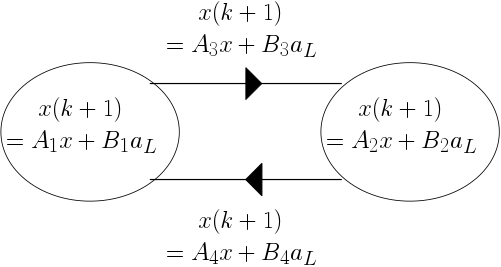
\includegraphics[scale=0.5]{fig/platton-dynamics.png}
\caption{Time discretized model of networked platoon}~\label{fig:model-platoon}
\end{figure}
%
%
\begin{table}
\caption{Matrices for discrete time slow switching model}~\label{matrices:slow}
{\scriptsize
$A_1=\mymatrix{0.2766  &  0.2855&   -0.0235&    0.2550&    0.2352&   -0.0429&    0.1245&    0.0956&   -0.0234\\
   -0.0917&   -0.0848&    0.0392&   -0.0517&    0.0134&    0.0023&    0.0003&    0.0385 &  -0.0166\\
   -0.0531&   -0.0485&    0.0404&    0.0434&    0.0807&   -0.0172&    0.0301&    0.0363&   -0.0097\\
    0.1406&    0.1632&    0.0002&    0.0313&    0.1166&   -0.0122&    0.1017&    0.1309&   -0.0431\\
   -0.0411&   -0.0589&   -0.0421&   -0.0512&   -0.1530&    0.0575&   -0.0476&   -0.0321&    0.0051\\
   -0.0393&   -0.0402&   -0.0111&   -0.0641&   -0.0754&    0.0467&    0.0497&    0.0760&   -0.0251\\
    0.0628&    0.0763&    0.0095&    0.0634&    0.0987&    0.0081&   -0.0788&    0.0489&   -0.0436\\
   -0.0088&   -0.0158&   -0.0081&   -0.0351&   -0.0452&   -0.0726&   -0.0621&   -0.2082&    0.0863\\
   -0.0246&   -0.0235&   -0.0078&   -0.0572&   -0.0547&   -0.0183&   -0.1049&   -0.1146&    0.0307}$
$A_2=\mymatrix{ 0.2398 &   0.2204&   -0.0715&   -0.0000&    0.0000&   -0.0000&   -0.0000&    0.0000&   -0.0000\\
   -0.1148&   -0.1083&    0.0352&   -0.0000&   -0.0000&    0.0000&   -0.0000&   -0.0000&    0.0000\\
   -0.0565&   -0.0567&    0.0176&   -0.0000&   -0.0000&   -0.0000&   -0.0000&   -0.0000&    0.0000\\
    0.0178&    0.5068 &  -0.0658&    0.2410&    0.3042&   -0.1113&   -0.0000&    0.0000&   -0.0000\\
   -0.1056&  -0.3026&    0.0327&   -0.1329&   -0.1627&    0.05657&   -0.0000&   -0.0000&    0.0000\\
   -0.1089&   -0.1100&   -0.0055&   -0.0675&   -0.0720&    0.0204&   -0.0000&   -0.0000&    0.0000\\
    0.2386&   -0.0802&    0.0965&    0.1118&    0.1544&    0.0604&    0.1197&    0.2679&   -0.1103\\
    0.0762&    0.3143&   -0.0998&   -0.0213&   -0.0283&   -0.0726&   -0.1404&   -0.2191&    0.0779\\
   -0.0043&    0.0212&   -0.0122&   -0.0468&   -0.0413&   -0.0171&   -0.0991&   -0.0990&    0.0251}$
 $B_1=\mymatrix{1.8593\\
    0.2855\\
    1.0848\\
    0.5394\\
    0.1632\\
    1.1437\\
    0.1950\\
    0.0763\\
    1.1596}$
$B_2=\mymatrix{1.7651\\
    0.2204\\
    1.1083\\
    2.1977\\
    0.5068\\
    1.4109\\
   -1.2748\\
   -0.0802\\
    1.0966}$
$B_3=\mymatrix{2.8411\\
    0.0019\\
    1.0006\\
    0.9508\\
    0.0007\\
    1.0009\\
    0.3775\\
    0.0003\\
    1.0009}$    
$B_4=\mymatrix{2.2276\\
    0.0001\\
    1.0001\\
    2.7152\\
   -0.0005\\
    1.0000\\
   -0.4469\\
    0.0001\\
    1.0000\\
}$
~~$A_3=A_4=\repmat{0}{9}{9}$.
}
\end{table}
%
\begin{table}
\caption{Matrices for discrete time fast switching model}~\label{matrices:fast}
{\scriptsize
$A_1=A_3=\mymatrix{ 0.8902 &   0.6370&   -0.1484&    0.0588&   -0.0050&    0.0001&    0.0157&   -0.0148&    0.0059\\
   -0.2340&    0.1889&   -0.1119&    0.1267&    0.0147&   -0.0039&    0.0363&   -0.0201&    0.0104\\
    0.1755&    0.7560&   -0.2251&   -0.0959&   -0.0989&    0.0181&   -0.0373&   -0.0273&    0.0018\\
    0.0462&    0.0643&    0.1514&    0.8509&    0.7076&   -0.1685&    0.0303&    0.0218&   -0.0038\\
    0.0934&    0.1271&    0.1151&   -0.3284&    0.2923&   -0.1466&    0.0660&    0.0517&   -0.0108\\
    0.1262&    0.6998&    0.0092&    0.1826&    0.7469&   -0.2119&   -0.0885&   -0.0830&    0.0189\\
    0.0116&    0.0170&    0.0026&    0.0241&    0.0282&    0.1719&    0.8532&    0.7238&   -0.1801\\
    0.0256&    0.0364&    0.0064&    0.0505&    0.0619&    0.1543&   -0.3320&    0.3231&   -0.1730\\
    0.1047&    0.6724&    0.0017&    0.1502&    0.6976&    0.0119&    0.2247&    0.7581&   -0.1875}$
$A_2=A_4=\mymatrix{0.8898 &   0.6325&   -0.1463&    0.0000&    0.0000&    0.0000&    0.0000&    0.0000&   -0.0000\\
   -0.2348&    0.1775&   -0.1094&    0.0000&    0.0000&    0.0000&    0.0000&    0.0000&   -0.0000\\
    0.1756&    0.7674&   -0.2136&    0.0000&    0.0000&    0.0000&    0.0000&    0.0000&   -0.0000\\
    0.0939&    0.3146&    0.1064&    0.9098&    0.6995&   -0.1686&    0.0000&    0.0000&   -0.0000\\
    0.1708&    0.6120&    0.0043&   -0.2012&    0.2985&   -0.1533&    0.0000&    0.0000&   -0.0000\\
    0.1687&    0.5757&    0.1151&    0.1829&    0.7569&   -0.1980&    0.0000&    0.0000&   -0.0000\\
   -0.0364&   -0.2331&    0.0460&    0.0254&    0.0312&    0.1721&    0.9004&    0.7304&   -0.1778\\
   -0.0529&   -0.4476&    0.1169&    0.0548&    0.0704&    0.1571&   -0.2263&    0.3541&   -0.1728\\
    0.1044&    0.6771&   -0.0016&    0.1418&    0.6953&    0.0121&    0.2199&    0.7571&   -0.1877}$    
$B_1=B_3=\mymatrix{0.3930\\
    0.6370\\
    0.8111\\
    0.0200\\
    0.0643\\
    0.6840\\
    0.0051\\
    0.0170\\
    0.6476\\
}$
$B_2=B_4=\mymatrix{0.3918\\
    0.6325\\
    0.8225\\
    0.0979\\
    0.3146\\
    0.2105\\
   -0.0727\\
   -0.2331\\
    0.6581}$
}
\end{table}
%

{\bf Time discretized models: } We could discretized the dynamics of
both models with large minimum switching time and integer switching
time.  The time discretized model has 2 locations and 4 edges, as
described in Figure~\ref{fig:model-platoon}.  The continuous state is
9-dimensional.  The matrices denoted in the figure are different for
the case of slow switching and fast switching and are given in
Tables~\ref{matrices:slow} and~\ref{matrices:fast}, respectively.


{\bf Linear invariance property: } The verification challenge proposed
in~\cite{makhlouf2014networked} is to find the minimum possible
reference distances $d_i^{ref}~\forall i\in\set{1,2,3}$, such that the
vehicles do not collide.  Any set of upper bounds on $-e_1$, $-e_2$,
and $-e_3$ are safe lower limits on the respective reference
distances.  We express the verification problem in terms of three
linear invariance properties, as follows.  For each ${T_i:~1\leq i\leq
3}$, where
%
$ T_1=\mymatrix{-1 & \repmat{0}{1}{8}},~
T_2=\mymatrix{\repmat{0}{1}{3} & -1 &\repmat{0}{5}{3}}$ and
 ${T_3=\mymatrix{\repmat{0}{1}{6}& -1 &\repmat{0}{2}{3}}},
$
%
find an upper bound on each $d_i:~i\in\set{1,2,3}$ such that
$\lt(T_i,d_i\rt)$ is a linear invariance property of the system.

\tbf{Experiment settings.}  We chose the primary template
as the collection of the (complex) eigenvectors of linear matrices of
the affine maps in the the two locations and their binary products,
the axis aligned box template and the templates used for
overapproximating the input sets. For the SpaceEx tool, we
experimented with two templates, octagon and hundred uniformly sampled
support vectors.

\tbf{Results.}  For the large minimum dwell time of $20s$, the
discrete time SpaceEx implementation and also a method based on using
real zonotopes~\cite{makhlouf2014networked} could verify slightly
smaller bounds compared to our approach.  But for the small minimum
dwell time ($1s$) model, SpaceEx could not even find a finite set of
bounds, whereas our approach could verify a finite set of bounds.  The
reason is that the fast system model is more stable compared to the
slow switching.  Possibly because complex zonotope captures
contraction along complex eigenvectors, we could find a finite
invariant for even the less stable fast switching model.  These
results are reported in the Tables~\ref{tab:largedwell-platoon}
and~\ref{tab:largedwell-platoon1}.
%

\begin{table}
\begin{tabular}{|l|c|c|c|c|c|}
\hline
\multicolumn{2}{|c|}{\multirow{4}{*}{Method}} & \multicolumn{4}{|c|}{\multirow{2}{*}{Slow switching}}\\
\multicolumn{2}{|c|}{} & \multicolumn{4}{|c|}{}\\
\cline{3-6}
\multicolumn{2}{|c|}{} & \multirow{2}{*}{$-e_1\leq$} & \multirow{2}{*}{$-e_2\leq$} & \multirow{2}{*}{$-e_3\leq$} & Comp.\\
\multicolumn{2}{|c|}{} & & & & time (s)\\
\hline
\multirow{4}{*}{SpaceEx} & octagon & \multirow{2}{*}{28} &
\multirow{2}{*}{27} & \multirow{2}{*}{10}& \multirow{2}{*}{$>180s$}\\
& template & & & &\\
\cline{2-6}
& 100 support & \multirow{2}{*}{28} & \multirow{2}{*}{25} &
\multirow{2}{*}{13} & \multirow{2}{*}{1.3}\\
& vectors & & & &\\
\hline
\multicolumn{2}{|c|}{\multirow{2}{*}{Real zonotope~\cite{makhlouf2014networked}}} &
\multirow{2}{*}{25} & \multirow{2}{*}{25} & \multirow{2}{*}{10} & \multirow{2}{*}{n/a}\\
\multicolumn{2}{|c|}{} & & & &\\
\hline
\multicolumn{2}{|c|}{\multirow{2}{*}{Augmented complex zonotope}} &
\multirow{2}{*}{28} & \multirow{2}{*}{26} &
\multirow{2}{*}{12} & \multirow{2}{*}{12}\\
\multicolumn{2}{|c|}{} & & & & \\
\hline
\end{tabular}
\caption{Experimental results: Slow switching networked platoon}~\label{tab:largedwell-platoon}

%% %
%% \end{table}
%% %
%% \begin{table}
{\vspace{2em}
\begin{tabular}{|l|c|c|c|c|c|}
\hline
\multicolumn{2}{|c|}{\multirow{4}{*}{Method}} & \multicolumn{4}{|c|}{\multirow{2}{*}{Fast switching}}\\
\multicolumn{2}{|c|}{} & \multicolumn{4}{|c|}{}\\
\cline{3-6}
\multicolumn{2}{|c|}{} & \multirow{2}{*}{$-e_1\leq$} & \multirow{2}{*}{$-e_2\leq$} & \multirow{2}{*}{$-e_3\leq$} & Comp.\\
\multicolumn{2}{|c|}{} & & & & time (s)\\
\hline
\multirow{4}{*}{SpaceEx} & octagon & \multirow{2}{*}{$>1000$} &
\multirow{2}{*}{$>1000$} & \multirow{2}{*}{$>1000$} &
\multirow{2}{*}{$>180s$}\\
& template & & & &\\
\cline{2-6}
& 100 support & \multirow{2}{*}{$>1000$} & \multirow{2}{*}{$>1000$} &
\multirow{2}{*}{$>1000$} & \multirow{2}{*}{$>180s$}\\
& vectors & & & & \\
\hline
\multicolumn{2}{|c|}{\multirow{2}{*}{Augmented complex zonotope}} &
\multirow{2}{*}{46} & \multirow{2}{*}{54} &
\multirow{2}{*}{57} & \multirow{2}{*}{12.6}\\
\multicolumn{2}{|c|}{} & & & & \\
\hline
\end{tabular}
%
\caption{Experimental results: Fast switching networked Platoon}~\label{tab:largedwell-platoon1}
}
\end{table}



\subsection{Perturbed double integrator}
Our second example is a perturbed double integrator system given
in~\cite{rakovic2004computation}.  The closed loop system with a
feedback control is piecewise affine, having four different affine
dynamics in four different regions of space, as
%
\begin{align*}~\label{eqn:pwa-regions}
& \trj{x}{t+1}=M_i\trj{x}{t}+w.~~~
 i=\left\{\begin{array}{l}
1,~\text{if}~x_1\geq 0~\text{and}~x_2\geq 0\\
2,~\text{if}~x_1\leq 0~\text{and}~x_2\leq 0\\
3,~\text{if}~x_1\leq 0~\text{and}~x_2\geq 0\\
4,~\text{if}~x_1\geq 0~\text{and}~x_2\leq 0\\
\end{array} \rt.,\\
&~M_1=M_2=\lt[\begin{matrix}
0.4103  &  0.0653\\
  -0.2949  &  0.5327
\end{matrix}\rt],~M_3=M_4=\lt[\begin{matrix}
0.4103  &  -0.0653\\
  0.2949  &  0.5327
\end{matrix}\rt].
\end{align*}

The additive disturbance input $w$ is bounded as $\|w\|_{\infty}\leq
0.2$.  

We perform two different experiments on this system.  In the first
experiment, we try to verify the smallest possible magnitude of bounds
on the two coordinates, denoted $x_1$ and $x_2$. We compare these
bounds with that found by the SpaceEx tool.  In the second experiment,
we try to quickly compute a large invariant for the system under the
safety constraints given in~\cite{rakovic2004computation}.  The given
safety constraints are $\|x\|_{\infty}\leq 5$.  In the latter case, we
maximize the sum of the scaling factors and differences of the upper
and lower interval bounds of the augmented complex zonotopic
invaraint.  Furthermore, we decompose the given safety constraints as
the intersection of four different sets of safety constraints.  For
each set of safety constraints, we compute a large augmented complex
zonotopic invariant.  Then the desired invariant is the intersection
of four augmented complex zonotopic invariants.  Although we may not
find the largest possible (maximal) invariant by this approach, still
the optimizer will try to maximize the size of the invariant.  We draw
comparison in terms of the computation time with the reported result
for the MPT tool~\cite{rakovic2004computation}.

In our formalism, we model the system with $4$ locations and $12$
edges connecting all the locations.  Appropriate staying conditions
are specified in each location, reflecting the division of the state
space into different regions where the dynamics is affine. The initial
set is the origin. The same model is specified in SpaceEx.

\tbf{Size of model}: 2 dimensions, 4 locations and 12 edges.

\tbf{Experiment settings}.  For the primary template, we collected the
(complex) eigenvectors of all linear matrices of the affine maps and
their binary products. For the SpaceEx tool, we experimented with two
different templates, the octagon template and a template with 100
uniformly sampled support vectors.

\tbf{Results.}  In the first experiment, we verified sligtly smaller bounds
for $x_1$ than that of SpaceEx, while the bounds verified for $x_2$
were equal for both methods.  In our second experiment on this
example, the computation time for finding a large invariant by our
method is significantly smaller than that of the reported result for
the MPT tool.  The results are summarized in the
Tables~\ref{tab:smallinv-pdi} and~\ref{tab:largeinv-pdi}.

\begin{table}
\center
\begin{tabular}{|l|c|c|c|c|}
\hline
\multicolumn{2}{|c|}{\multirow{2}{*}{Method}} &
\multirow{2}{*}{$\lt|x_1\rt|\leq$} & \multirow{2}{*}{$\lt|x_2\rt|\leq$} & Comp.\\
\multicolumn{2}{|c|}{} & & & time (s) \\
\hline
\multirow{4}{*}{SpaceEx} & octagon & \multirow{2}{*}{0.38} &
\multirow{2}{*}{0.43} & \multirow{2}{*}{1.7}\\
& template & & &\\
\cline{2-5}
& 100 support & \multirow{2}{*}{0.38} & \multirow{2}{*}{0.43} & \multirow{2}{*}{23.6}\\
& vectors & & &\\
\hline
\multicolumn{2}{|c|}{\multirow{2}{*}{ACZ invariant}} &
\multirow{2}{*}{0.37} & \multirow{2}{*}{0.43} & 
\multirow{2}{*}{5.1}\\
\multicolumn{2}{|c|}{} & & &\\
\hline
\end{tabular}
\caption{Small invariant computation: Perturbed double
  integrator}
~\label{tab:smallinv-pdi}
\end{table}
%
\begin{table}
\center
\begin{tabular}{|c|c|}
\hline
\multirow{2}{*}{Method} & Comp.\\
& time (s)\\
\hline
\multirow{2}{*}{MPT tool~\cite{rakovic2004computation}} & \multirow{2}{*}{107}\\
& \\
\hline
\multirow{2}{*}{ACZ} & \multirow{2}{*}{12}\\
& \\
\hline
\end{tabular}
\caption{Large invariant computation: Perturbed double integrator}
~\label{tab:largeinv-pdi}
\end{table}
%% \tbf{Remark.}  The overapproximation quality of SpaceEx reduces when
%% there are large number of edges, because then in each step, a union of
%% many different polytopes has to be overapproximated using support
%% vectors.  In contrast, our approach uses optimization to learn an
%% appropriate invariant, avoiding the union operations.  Possibly
%% because of this reason, we verified smaller bounds than SpaceEx on
%% this example.



%
\chapter{Conclusion} \label{ch:conclusion} %\vspace{-em}
\section{Conclusion}
\vspace{0em}
We extended complex zonotopes to template complex zonotopes in order to
improve the efficiency of the computation of contractive sets and
positive invariants.  Template complex zonotopes retain a useful feature of complex zonotopes, which is the scope to incorporate the
eigenvectors of linear dynamics among the generators because the
eigenstructure is related to existence of positive
invariants.  In addition, compared to complex zonotopes, the advantage
template complex zonotopes have is the ability to regulate the
contribution of each generator to the set by using the scaling factors.
This resulted in significantly improved verification of stability of
nearly periodic impulsive systems, and also extending its application
to switched systems for verification of linear invariance properties.
The advantage of this new set representation is attested
by the experimental results that are better or competitive, compared
to the state-of-the-art methods and tools on benchmark examples. This
work also contributes a method for exploiting the eigenstructure of
linear dynamics to algorithmically determine template directions,
required by most verification approaches using template sub-polyhedral
sets. A number of directions for future research can be
identified. First, we intend to extend these techniques to analysis to
switched systems under constrained switching laws. Also
computationally speaking, our approach is close in spirit to abstract
interpretation. Indeed the operations used to find positive invariants and contractive sets
can be extended to invariant computation for more general hybrid
systems with state-dependent discrete transitions.
%to the way invariant sets are computed using some zonotopic

%and hybrid systems analysis. Indeed the way we find contractive sets using such zonotopes is similar 
%to the way invariant sets are computed using some zonotopic
%\cite{Girard05reachabilityof,Althoff2011,DBLP:conf/sas/GoubaultPV12} and
%template-polyhedral abstract domains \cite{S riram2008,jeannet2009apron}.

%  


%% \appendix
%% \chapter{Appendix} 
%\section{Proofs in Section~\ref{}}
%
\subsection*{Proof of Lemma~\ref{lem:motivation}}
\begin{proof}
Firstly, we prove $\zon{\pinv{K}}{l}{u} \bigcap
\sptope{K}{\wh{l}}{\wh{u}} \subseteq \zon{K}{l\bigvee
  \wh{l}}{u\bigwedge \wh{u}}$.  Let $x\in\zon{\pinv{K}}{l}{u} \bigcap
\sptope{K}{\wh{l}}{\wh{u}}$.  Then, $x=\pinv{K}\zeta:
\wh{l}\leq\zeta\leq \wh{u}$.  Since $x\in\sptope{K}{\wh{l}}{\wh{u}}$, so
$l\leq K\lt(\pinv{K}\zeta\rt)\leq u$ $\dimp$ $l\leq \zeta\leq u$.  So,
$l\bigvee \wh{l}\leq \zeta\leq u\bigwedge\wh{u}$.  Hence, $x\in\zon{K}{l\bigvee
  \wh{l}}{u\bigwedge \wh{u}}$.

Next, we show $\zon{\pinv{K}}{l}{u} \bigcap \sptope{K}{\wh{l}}{\wh{u}}
\supseteq \zon{K}{l\bigvee \wh{l}}{u\bigwedge \wh{u}}$. Let
$x=\pinv{K}\zeta\in\zon{K}{l\bigvee \wh{l}}{u\bigwedge \wh{u}}$.
Then, $l\bigvee\wh{l}\leq \zeta = K\lt(\pinv{K}\zeta\rt)=Kx\leq
u\bigwedge\wh{u}$.  Since $l\leq l\bigvee\wh{l} \zeta\leq u\bigwedge
\wh{u}\leq u$, so $x\in \zon{\pinv{K}}{l}{u}$.  Since $\wh{l}\leq
l\bigvee\wh{l} Kx\leq u\bigwedge \wh{u}\leq \wh{u}$, $x\in
\zon{\pinv{K}}{l}{u}$, so $x\in\sptope{K}{\wh{l}}{\wh{u}}$.
\end{proof}

\subsection*{Matrices in the first benchmark (robot with a saturated controller)}
{\scriptsize 
\begin{align*}
& F_1  = \lt[\begin{matrix}
3.6929   &      0  &  0.7302  &  7.9715 &  14.5019 &   -0.0072 &
0.0720 &   -2.7354\\
    3.6929   &      0  &  0.7302  &  7.9715 &  14.5019 &  -0.0072  &  0.0720  & -2.7354\\
    0.9562    &     0  &  0.0019 &  -0.0021 &  -0.0022 &   -0.0000 &  -0.0001 &  -0.0002\\
         0 &   0.6910    &     0    &     0  &       0     &    0   &      0    &     0\\
    0.8833     &    0  & -0.1154 &  -1.2943 &  -2.3520  &  0.0012 &  -0.0118  &  0.4427\\
   -0.4712    &     0 &  -0.0812 &    0.1151  & -1.4845  &  0.0007 &  -0.0071  &  0.2819\\
   -0.1560     &    0 &  -0.0459 &  -0.3173  &  0.3650  &  0.0003  & -0.0023  &  0.1162\\
   -0.7719   &      0 &  -0.1248  & -1.4264 &  -2.5901  &  0.9973 &  -0.0131  &  0.4869\\
   -0.7544  &       0  & -0.1243 &  -1.4204 &  -2.5792  &  0.0013 &   0.9825 &   0.4796\\
   -0.1905   &      0  & -0.0148  & -0.2081 &  -0.3751  &  0.0002  &  0.0033  &  1.0651
\end{matrix}\rt]\\
& F_2 = \lt[\begin{matrix}
0.2543  &  0.2543\\
    0.2543  &  0.2543\\
   -0.0001 &  -0.0001\\
         0 &        0\\
   -0.0413 &  -0.0413\\
    0.0219  &  0.0219\\
    0.0102 &   0.0102\\
    0.0431 &   0.0431\\
    0.0428 &   0.0428\\
    0.0065 &   0.0065\\
\end{matrix}\rt],
~F_3 = 10^{-2}\times\lt[\begin{matrix}
 0.0000    &     0  & -0.0330 &   2.0218\\
    0   &      0  & -0.0330 &  -2.0218\\
    0  &       0 &   -0  &  0\\
   -0  &       0  &  0 &   0.0109\\
   -0.0118 &        0  &  0.0172  &  0 \\
    0.0436  &       0 &   0.0003 &  0 \\
   -0.0478   &      0  &  0.0034 &   0 \\
  -13.3924 &        0 &   0.0062 &   0 \\
    0.0909     &    0  &  0.0061 &  0\\
   -0.0798  &       0 &   0.0017  &  0\\
\end{matrix}\rt]
\end{align*}}

\subsection*{Matrices in the second benchmark (perturbed double integrator)}
{\scriptsize
\begin{align*}~\label{eqn:pwa-regions}
i=\left\{\begin{array}{l}
1,~\text{if}~x_1\geq 0~\text{and}~x_2\geq 0\\
2,~\text{if}~x_1\leq 0~\text{and}~x_2\leq 0\\
3,~\text{if}~x_1\leq 0~\text{and}~x_2\geq 0\\
4,~\text{if}~x_1\geq 0~\text{and}~x_2\leq 0\\
\end{array} \rt.,
~M_1=M_2=\lt[\begin{matrix}
0.4103  &  0.0653\\
   -0.2949  &  0.5327
\end{matrix}\rt],~M_3=M_4=\lt[\begin{matrix}
0.4103  &  -0.0653\\
   0.2949  &  0.5327
\end{matrix}\rt]
\end{align*}}

% \backmatter
\addcontentsline{toc}{chapter}{Bibliography}
% plain alpha abbrv acm apalike ieeetr siam unsrt
\bibliographystyle{alpha}
\bibliography{./myLib,reflis}

%%% Here goes a list of acronyms (if needed)

%%% Here goes the Index
% \printindex

\end{document}
